\documentclass[a4paper,8pt,oneside,openany]{jsbook}
%
\usepackage{amsmath,amssymb}

\usepackage{bm}
\usepackage{subfigure}
\usepackage{verbatim}
\usepackage{wrapfig}
\usepackage{ascmac}
\usepackage{sidenotes}
\usepackage{makeidx}
\usepackage[dvipdfmx]{graphicx}
\usepackage{here}
\usepackage{tikz}
\usepackage{url}
\usepackage{mathrsfs}
\usepackage{braket}
\usepackage[many]{tcolorbox}
\usepackage[right=3cm]{geometry}
\usepackage[dvipdfm,colorlinks=true,urlcolor=blue]{hyperref}
\renewcommand{\contentsname}{Contents}
\renewcommand{\bibname}{References}
\renewcommand{\appendixname}{Appendix~}

\usepackage{layout}

\usepackage[explicit]{titlesec}
\usepackage{lipsum}



\titleformat{\chapter}[block]
  {\normalfont\huge\bfseries}
  {\tikz\node[
      font=\huge\bfseries\color{white},
      fill=gray!50,
      rounded corners=20pt,
      minimum height=1.6cm,
      text width=3em,
      align=center,
      inner xsep=0pt] {\parbox{1.5em}{\thechapter\hfill}};%1の位置を定めている.
  }
  {-0.5em}%灰色域の
  {\tikz\node[
      fill=gray,
      font=\Large\sffamily\color{white},
      minimum height=1.6cm,
      text width=\the\dimexpr\textwidth-2em\relax,%灰色の文字の中身を
      align=center,inner xsep=-10pt] {#1};%
  }


  \titleformat{\chapter}[block]
  {\normalfont\huge\bfseries}
  {\tikz\node[
      font=\huge\bfseries\color{white},
      fill=gray!50,
      rounded corners=20pt,
      minimum height=1.6cm,
      text width=3em,
      align=center,
      inner xsep=0pt] {\parbox{1.5em}{\thechapter\hfill}};%1の位置を定めている.
  }
  {-1em}%灰色域の
  {\tikz\node[
      fill=gray,
      font=\Large\sffamily\color{white},
      minimum height=1.6cm,
      text width=\the\dimexpr\textwidth-2em\relax,%灰色の文字の中身を
      align=center,inner xsep=-10pt] {#1};%
  }


\titleformat{name=\chapter,numberless}[block]
  {\normalfont\huge\bfseries}
  {\tikz\node[
      font=\huge\bfseries\color{white},
      fill=gray!50,
      rounded corners=20pt,
      minimum height=1.6cm,
      text width=3em,
      align=center,
      inner xsep=0pt] {\parbox{1.5em}{\mbox{}\hfill}};%
  }
  {-1em}
  {\tikz\node[
      fill=gray,
      font=\Large\sffamily\color{white},
      minimum height=1.6cm,
      text width=\the\dimexpr\textwidth-2em\relax,
      align=center,
      inner xsep=0pt] {#1};%
  }

  \titleformat{\section}[block]
  {\normalfont\large\bfseries}
  {\tikz\node[
      font=\large\bfseries\color{black},
      fill=white,
      rounded corners=20pt,
      minimum height=1.6cm,
      text width=10em,
      align=center,
      inner xsep=0pt] {\parbox{-0.5em}{\thesection}};%1の位置を定めている.
  }
  {-3em}%灰色域の
  {\tikz\node[
      fill=white,
      font=\Large\sffamily\color{black},
      minimum height=1.6cm,
      text width=\the\dimexpr\textwidth-12em\relax,%灰色の文字の中身を
      align=center,inner xsep=-10pt] {#1};%
  }

\setcounter{tocdepth}{2}
\hypersetup{%
linkcolor=blue%
}%
\hypersetup{%
citecolor=blue%
}%

\newtcolorbox{empheqboxed}[1][]{colback=gray!20,
 colframe=white,
 width=\textwidth,
 sharpish corners,
 top=-3mm, % default value 2mm
 bottom=3pt
}
\def\id#1{\def\@id{#1}}
\usetikzlibrary[arrows,decorations.pathmorphing,backgrounds,positioning,fit,petri]
\usetikzlibrary{intersections,calc}
\newcommand{\bvec}[1]{\mbox{\boldmath$#1$}}
%
\makeindex
%

%
\newcommand{\diff}{\mathrm{d}}  %微分記号
\newcommand{\divergence}{\mathrm{div}\,}  %ダイバージェンス
\newcommand{\grad}{\mathrm{grad}\,}  %グラディエント
\newcommand{\rot}{\mathrm{rot}\,}  %ローテーション
%
\title{量子情報}
\author{川 大揮}
\id{17M00430}
\date{\today}
\begin{document}
%
%
%\maketitle
\begin{titlepage}
\begin{flushright}
{\large
指導教員(主査):山口昌英 教授  % 主査
}
\end{flushright}
\begin{center}
\vspace*{150truept}
{\huge \textit{量子情報}}\\ % タイトル
\vspace{120truept}
{\Large17M00430}\\ % 学籍番号
\vspace{50truept}
{\Large 川 大揮}\\ % 著者
\vspace{50truept}
{\today}\\ % 提出日
\end{center}
\end{titlepage}
%
%
\frontmatter
%
\addcontentsline{toc}{chapter}{}
\section{Notation}
$-++++$

\tableofcontents
%
%
\mainmatter
%
\layout
\chapter{量子情報理論の基礎}

\section{Motivation}
量子情報の分野では,全体と部分系を分けることで新たの視点や混合状態などが現れる.
そこで,このような全体と部分という視点は,いつも意識しておく必要がある.(CP-mapもPOVMもそれに当たる.)

物理学の統一理論を作りたいが重力だけがまだ統一できていない.具体的には,重力の量子化を行うと高エネルギー領域の量子揺らぎによって起こる紫外発散が頻繁に起こるため量子論として大きな問題が生じる.これは,粒子が点であるとみなすことによって起因するものであると思われている.そこで有限の大きさをもつヒモとして扱う超弦理論は,統一理論の有力な候補として考えられてきた.

ミクロな量子論に問題がある一方,マクロな重力現象にもミステリアスな現象が起こる.統計力学では,識別できない情報量をエントロピーで表す.実は,ブラックホールにも,このエントロピーがあることが知られている.さらに,BHには温度が定義できて熱力学法則も満たすことがわかってきた.(ブラックホール熱力学)

ブラックホールのエントロピー$S_{BH}$は,次の有名なベッケンシュタインホーキングの面積公式
\begin{align}
  S_{BH}=\frac{k_{B}c^3}{4G_{N}\hbar}A
\end{align}
で与えられる.ここで,$A$はBHの表面積である.この式には,様々な物理定数が現れる.重力理論の重力定数,統計力学のボルツマン定数,量子力学のプランク定数が用いられる.言い換えるとこの理論,または公式を本当に理解するためには,これら三つの分野をきちんと融合し量子重力理論を構築する必要がある.

熱力学とブラックホール物理との間には類似性があり,
\begin{center}
内部エネルギーと質量 \\
温度と表面重力\\
エントロピーと面積
\end{center}
それぞれ対応する.これらの対応関係に基づいて,Bekenstein は情報理論の観点 からブラックホールがエントロピーを持つことを示唆した.情報理論では,情報の損失はエントロピーの増加を意味する.ここでは,ある物体がブラックホールに落ち込むことを考える.物体がブ ラックホールに落ち込む前,我々は物体についての情報を知ることができるが,一度,物体がブラッ クホールに落ち込むと,その物体がどういう状態にあるのか我々は物体に対する全ての情報を失うこ とになる.この失われた情報がブラックホールのエントロピーの増加になると考え,ブラックホール が大きなエントロピーを持つことを提案した.そして,そのエントロピーの増加が物体が落ち込むことによって増加するブラックホールの表面積の増加と結び付けた.彼はブラックホールがエントロピーを持つことは示唆したが,温度を持つことまでは提案しなかった.その理由はブラックホールの定義である「どんな粒子の放出を許さない閉鎖的な領域」であることに起因する.ブラックホールが温度を持つ場合,周囲の温度との比較によっては,熱吸収だけではなく,熱放射も説明しなければならない.Bekensteinはブラックホールの放射のメカニズムを説明するまでには至らず,ブラックホー ルが温度を持つとまでは言えなかった.
Bekenstein の論文を受けてHawkingはブラックホールの放射のメカニズムを探し,場の量子論の考察からブラックホール放射のメカニズムを考案した.具体的にはBogoliubov変換を用いて粒子数の期待値がボルツマン分布に従うことを示した,また,熱力学のアナロジーとして温度も定義できる.この特別なブラックホールの温度は,Hawking温度と呼ばれている.Hawkingによりブラックホール放射のメカニズムが明らかとなったため,ブラックホー ル物理と熱力学との間に完全な対応関係を与えることが可能となった.


また,公式からもわかるように,BHのエントロピーは示量変数であるのにも関わらずその体積でなく(通常の統計力学では,エントロピーは体積に比例する)BHの表面積に比例している.(BHのホライズンはほぼ球対称)これは,我々がしる物質とは異なる性質を示しどうしてBHのエントロピーが表面積に比例するのか,あるいはBHのエントロピーとは一体何なのかよくわかっていない.このように,マクロな視点でも解決されていない問題がある.


先ほど述べたように,ブラックホールのエントロピーはBHの中の情報が見れないことによると考えられる.重力を忘れて純粋な量子力学を考えると,量子系の一部が観測できないことによって生じるエントロピーは,エンタングルメントエントロピーと呼ばれる.(量子力学の情報を定式)
そこで,ブラックホールのエントロピーを理解するだ一歩として場の理論におけるエンタングルメントエントロピーを計算する研究が盛んに行われるようになった.(1980年)
(今までのBHのエントロピーの導出は,BHの粒子生成を考えてその粒子数密度から(アナロジー的に)温度を定義してそれを下に,熱的にエントロピーを求めたがそれを量子力学的なアプローチで求めようとする試みである.(これがうまくいくってことは量子力学の中にもう温度という概念が含まれているのか)
\subsection{重力のエントロピーとエンタングルメントエントロピー}
ブラックホールのエントロピーとエンタングルメントエントロピーの類似性は,80年代から議論が進んいる.
重力のエントロピーは,量子力学(場の量子論)のエンタングルメントエントロピーと関係があることを高柳さんたちは示した.これによると,量子場の理論におけるエンタングルメントエントロピーは,一つ次元の高い重力の理論の言葉で書くことができる.


疑問は,重力のエントロピーを知りたかったら,その理論の境界の場の理論のエントロピーを求めれば良いのか??

そうみたいだ.
マルダセナの論文では,だから注意書きがされている.これからやりたいのは,重力のエントロピーを求めたいわけでなない.pureに場の理論における量子相関を求めたいわけである.


\subsection{ホログラフィー原理}
ある時空$\mathcal{M}$における,重力理論は,その境界$\mathcal{\partial M}$における重力理論を含まない場の理論に等価である.
\subsection{AdS/CFT}
反de Sitter時空における量子重力理論は,その境界上の共形場理論に等価である
\subsection{first theses}
Minkowski時空における量子エンタングルメントは,時空の次元によるのものなのか
\section{純粋状態と混合状態}
\subsection{純粋状態におけるエンタングルメント}
純粋状態とは,量子状態$\ket{\phi}$が非自明な確率混合で準備できない状態である.すなわち,Density Matrixが,
\begin{equation}
\label{1}
\rho=\ket{\phi}\bra{\phi}
\end{equation}
の形で与えられる場合である.(\ref{1})式から,純粋状態であれば,
\begin{equation}
\rho^{2}=\rho=1
\end{equation}
が成立する.
\begin{empheqboxed}
  \
  \

  純粋状態$\ket{\phi}$が,エンタングルしてないすなわち,セパラブル(separable)であるときは,
  \begin{equation}
    \label{3}
  \ket{\phi}=\frac{1}{2}(\ket{\uparrow}_{A}+\ket{\downarrow}_{A})(\ket{\uparrow}_{B} +\ket{\downarrow}_{B})=\ket{A}\otimes\ket{B}
  \end{equation}

\end{empheqboxed}

のように,2つの系全体の量子状態が部分系$A,B$の直積として表現できるときである.これに対して,
\begin{empheqboxed}
\
\

エンタングルしている状態としては,
\begin{equation}
    \label{4}
    \ket{\phi_{Bell}}=\frac{1}{\sqrt{2}}(\ket{\uparrow}_{A}\ket{\uparrow}_{B}+\ket{\downarrow}_{A}\ket{\downarrow}_{B})
    \end{equation}
    のように直積で書くことのできない状態である.
\end{empheqboxed}
(\ref{4})式にあげた例は,Bell状態と呼ばれ,
この状態に関するエントロピー,すなわちエンタングルメントエントロピー$S(\rho)$
\begin{empheqboxed}
\

\begin{equation}
S(\rho)=-Tr(\rho_{A}\ln \rho_{A})
\end{equation}
\end{empheqboxed}
を最大にし,さらにベルの不等式を最大で破っている場合になっている.ただし,$\rho_A$は,Density MatrixでBについてPartial Traceを取ったもので,
\begin{equation}
\rho_{A}={Tr}_{B}\rho
\end{equation}

で定義される.このように,純粋状態は,片方の状態をPartial Traceをとることでエンタングルメントエントロピーが計算でき,エンタングルしているかどうかを判定することができる.

そのために,混合状態について言及しておく.
\subsection{混合状態におけるエンタングルメントエントロピー}

\textcolor[rgb]{0.4,0.4,0.4}{\begin{align*}
\mathcal{H}_{tot}=\mathcal{H}_{A}\otimes\mathcal{H}_{A}
\end{align*}}


1つの物理系についても,純粋状態と混合状態が定義できる.混合状態と純粋状態では,密度行列の数学的な性質が異なる.例えば,separableな状態である(\ref{3})から構成した密度行列は,
\begin{align}
  \rho^{AB_{p}}=\frac{1}{4}(&\ket{\uparrow}_{A}\ket{\uparrow}_{B}+\ket{\downarrow}_{A}\ket{\uparrow}_{B}+\ket{\uparrow}_{A}\ket{\downarrow}_{B}+\ket{\downarrow}_{A}\ket{\downarrow}_{B})
  (\bra{\uparrow}_{A}\bra{\uparrow}_{B}+\bra{\downarrow}_{A}\bra{\uparrow}_{B}+\bra{\uparrow}_{A}\bra{\downarrow}_{B}+\bra{\downarrow}_{A}\bra{\downarrow}_{B}) \nonumber \\
  =\frac{1}{4}(
&\ket{\uparrow}_{A}\ket{\uparrow}_{B}\bra{\uparrow}_{A}\bra{\uparrow}_{B}+\ket{\downarrow}_{A}\ket{\uparrow}_{B}\bra{\uparrow}_{A}\bra{\uparrow}_{B}+\ket{\uparrow}_{A}\ket{\downarrow}_{B}
\bra{\uparrow}_{A}\bra{\uparrow}_{B}+\ket{\downarrow}_{A}\ket{\downarrow}_{B}\bra{\uparrow}_{A}\bra{\uparrow}_{B}\nonumber \\
&+\ket{\uparrow}_{A}\ket{\uparrow}_{B}\bra{\downarrow}_{A}\bra{\uparrow}_{B}+\ket{\downarrow}_{A}\ket{\uparrow}_{B}\bra{\downarrow}_{A}\bra{\uparrow}_{B}+\ket{\uparrow}_{A}\ket{\downarrow}_{B}
\bra{\downarrow}_{A}\bra{\uparrow}_{B}+\ket{\downarrow}_{A}\ket{\downarrow}_{B}\bra{\downarrow}_{A}\bra{\uparrow}_{B}\nonumber \\
&+\ket{\uparrow}_{A}\ket{\uparrow}_{B}\bra{\uparrow}_{A}\bra{\downarrow}_{B}+\ket{\downarrow}_{A}\ket{\uparrow}_{B}\bra{\uparrow}_{A}\bra{\downarrow}_{B}+\ket{\uparrow}_{A}\ket{\downarrow}_{B}
\bra{\uparrow}_{A}\bra{\downarrow}_{B}+\ket{\downarrow}_{A}\ket{\downarrow}_{B}\bra{\uparrow}_{A}\bra{\downarrow}_{B}\nonumber \\
&+\ket{\uparrow}_{A}\ket{\uparrow}_{B}\bra{\downarrow}_{A}\bra{\downarrow}_{B}+\ket{\downarrow}_{A}\ket{\uparrow}_{B}\bra{\downarrow}_{A}\bra{\downarrow}_{B}+\ket{\uparrow}_{A}\ket{\downarrow}_{B}
\bra{\downarrow}_{A}\bra{\downarrow}_{B}+\ket{\downarrow}_{A}\ket{\downarrow}_{B}\bra{\downarrow}_{A}\bra{\downarrow}_{B}
)
\end{align}
となるが,この式でBに関する物理系をトレースアウトすれば,

\begin{align}
  \rho^{A_{p}}&=\rm{Tr}\rho^{AB_{p}} \\
  &=\frac{1}{2}(
\ket{\uparrow}_{A}\bra{\uparrow}_{A}+\ket{\uparrow}_{A}\bra{\downarrow}_{A}+\ket{\downarrow}_{A}\bra{\uparrow}_{A}+\ket{\downarrow}_{A}\bra{\downarrow}_{A})\\
&=\frac{1}{2}(\ket{\uparrow}_{A}+\ket{\downarrow}_{A})(\bra{\uparrow}_{A}+\bra{\downarrow}_{A})
\end{align}
となり,これは,Aの物理系だけの純粋状態$\bra{\psi}=\frac{1}{\sqrt{2}}(\ket{\uparrow}_{A}+\ket{\downarrow}_{A})$になっていることがわかる.これは,\textbf{separableな状態においてBの物理系ををトレースアウトすれば,Aの純粋状態だけが残る}という非常に当たり前の結果である.また,純粋状態の密度演算子は,二乗すると元に戻るので,
\begin{align}
  \rho^2=\rho,\hspace{2mm}\rm{Tr}\rho^2=1
\end{align}
などの性質がある.次に,entangleな状態から構成される量子状態について考える.


混合状態は,エンタングル状態の2つの物理系から1つをトレースアウトすることで得られる.



混合状態は,純粋状態でない状態すなわち,量子状態$\ket{\phi}$が非自明な確率混合で準備できる状態である.
混合状態では,非自明な確率で様々な量子状態が混合されている状態である,
\begin{equation}
\rho=\sum_{i}p_i\rho_{i}
\end{equation}
\begin{empheqboxed}
  \
  \

  混合状態がセパラブルであるとは,
  \begin{equation}
  \label{30}
  \rho=\sum_{i}p_i\rho^{A}_{i}\otimes\rho^{B}_{i}=\sum_{i}p_i\ket{i}_A\bra{i}_{A}\otimes\ket{i}_B\bra{i}_{B}
  \end{equation}
  と書けるときである.
\end{empheqboxed}
separabilityについて詳しく考える。セパラブルな状態は、後述のLOCCによって生成される

一方,一般的なDensity Matrixは,
\begin{eqnarray}
\label{40}
\rho=\sum_{ijkl}C_{ijkl}\ket{i}_A\bra{j}_{A}\otimes\ket{k}_B\bra{l}_{B}
\end{eqnarray}
で表される.
\textcolor{red}{以上のことと,fedelty,bell inequolity,traceの値などを次のような表にまとめておくと便利かも.}\footnote{ここでは,2つの物理系のエンタングルメントを考えているが,純粋状態と混合状態は1つの物理系のみで定義できることにも注意したい.また,表記の便宜上純粋状態に関しては,密度行列で書いていないので注意していただきたい.}
{\renewcommand{\arraystretch}{2}
\begin{table}[H]
  \begin{center}
    \begin{tabular}{c|c|c}
       & pure state & mixed state  \\\hline
      separable & $ \ket{\phi}=(\ket{\uparrow}_{A}+\ket{\downarrow}_{A})(\ket{\uparrow}_{B} +\ket{\downarrow}_{B})$ & $\rho=\sum_{i}p_i\rho^{A}_{i}\otimes\rho^{B}_{i}$ \\\hline
      entangle &    $\ket{\phi_{Bell}}=(\ket{\uparrow}_{A}\ket{\uparrow}_{B}+\ket{\downarrow}_{A}\ket{\downarrow}_{B})$  & $\rho=\sum_{i}p_i\rho^{AB}_{i}$
    \end{tabular}
  \end{center}
  \caption{title}
\end{table}}

混合状態では,上と同じ方法を取ってもセパラブル状態でもエンタングルメントエントロピーが$0$とはならいことがある.
そこで,エンタングルメントエントロピーを測度として用いられない.
\begin{empheqboxed}
  \
  \

  pure stateのエンタングルメント判定方法は,次のようにまとめられる.

  \begin{align}
    S(\rho^{A})=0, \hspace{4mm} then\ the\ state\ is\ separable\\
    S(\rho^{A})\neq0, \hspace{4mm} then\ the\ state\ is\ entangle
  \end{align}
\end{empheqboxed}

\section{PPT条件とNegativity}
混合状態や,3つ以上の量子もつれにも適用できる測度としてNegativityがある,\footnote{Negativityが最良の測度であるという意味ではない.}PPT(Positive Partial Transpose)条件は,Density Matrix\ $\rho$に対して,
\begin{eqnarray}
\label{5}
\rho^{T_{A}}
\end{eqnarray}
の固有値が符号によってエンタングルしているか否かを判定する,ここで,上つきの$T_{A}$は,Partial Transpose(部分転置)で,一般的な混合状態(\ref{40})式に適応すると,
\begin{eqnarray}
\label{6}
\rho^{T_{A}}=\sum_{ijkl}C_{ijkl}\ket{j}_A\bra{i}_{A}\otimes\ket{k}_B\bra{l}_{B}
\end{eqnarray}
のように,Aに関してのみ転置を取ることを意味する.(\ref{30})式に適応すれば,
\begin{eqnarray}
\rho^{T_{A}}=\sum_{i}p_{i}\ket{i}_A\bra{i}_{A}\otimes\ket{i}_B\bra{i}_{B}=\rho
\end{eqnarray}
となり,セパラブルな状態であればその固有値は元のDensity Matrixの固有値$1$に等しく正の値となる.
これに対して,セパラブルで書けない,エンタングルしているときは,固有値が負の値になる.\footnote{エンタングルしていても,固有値が正になるときもある.現在までに提案されている様々な測度はエンタングルしているものを全て判定できるわけだはない.}
\subsection{Negativity}
Negativity $N$を(\ref{5})式で定義されたensity Matrixの負の固有値の総和として,
\begin{eqnarray}
N=\sum_{\lambda_{i<0}}|\lambda_i|
\end{eqnarray}
で定義する.ここで,$\lambda$は$\rho^{T_{A}}$の固有値である.さらに,Matrix $X$のTrace Normを次で定義する.
\begin{eqnarray}
||X||=\rm{Tr}\sqrt{X^{\dagger}X}
\end{eqnarray}
すると,$\rho^{T_{A}}$のTrace Normは,
\begin{eqnarray}
\label{7}
||\rho^{T_{A}}||=\sum_{i}|\lambda_{i}|=\sum_{\lambda_{i<0}}|\lambda_i|+\sum_{\lambda_{i<0}}|\lambda_i|
\end{eqnarray}
となる,いま,(\ref{6})式から,
\begin{eqnarray}
\rm{Tr}\rho=\rm{Tr}\rho^{T_{A}}
\end{eqnarray}
であることがわかるので,固有値の総和は,もとのDensity Matrixの固有値の総和$1$に等しく$\sum_{i}\lambda_i$である.したがって,
\begin{eqnarray}
\sum_{\lambda_{i<0}}|\lambda_i|-\sum_{\lambda_{i\leqslant0}}|\lambda_i|=1
\end{eqnarray}
から,
\begin{eqnarray}
 \sum_{\lambda_{i<0}}|\lambda_i|=\sum_{\lambda_{i\leqslant0}}|\lambda_i|+1
\end{eqnarray}
が求まる.これを,(\ref{7})式に代入すれば,
\begin{eqnarray}
||\rho^{T_{A}}||=2\sum_{\lambda_{i\leqslant0}}|\lambda_i|+1
\end{eqnarray}
のように,Density MatrixとNegativityに関係が得られた.さらに,
\begin{eqnarray}
L(N)=\log||\rho^{T_{A}}||=\log(2N+1)
\end{eqnarray}
のように,対数を取れば,エンタングルメントエントロピーと同様の加法性などのせいなどの性質を満たす.この値をLogarithmic negativityという.
\section{量子力学と統計力学エントロピー}
\subsection{カノニカル・アンサンブル}
熱浴の中にある閉じた系で,ある微視的状態$n$が実現する確率は,
\begin{equation}
  \label{22}
  p_n=\frac{e^{-\beta E_n}}{\sum_{k}e^{-\beta E_k}}
\end{equation}
となる.このようなアンサンブル (分布) をカノニカル・アンサンブル(canonical ensemble,正準集団) あるいはカノニカル分布 (canonical distribution) と呼ぶ.(\ref{22})式の分母に含まれる和は,分配関数のと呼ばれ
\begin{equation}
  Z=\sum_{n}e^{-\beta E_n}
\end{equation}
で定義される,また,ヘルムホルツの自由エネルギー$F$と分配関数の関係は,
\begin{equation}
  F=-\frac{1}{\beta}\log Z
\end{equation}
の関係がある.はじめにこの関係について導出する.

-----村上さんのをみよ------



次に,統計に力学におけるエントロピーを確認する,
統計力学では,エントロピーはヘルムホルツの自由エネルギー$F$を用いて,
\begin{equation}
  S=\frac{1}{T}(E-F)
\end{equation}
で表すことができる.まずこれを示し,量子力学におけるエントロピーと統計力学におけるエントロピーの関係性について議論する.
混合状態における温度$T=\frac{1}{T}$のカノニカル分布の密度行列は,
\begin{eqnarray}
\label{25}
\rho_{tot}=\frac{e^{-\beta \mathcal{H}}}{Z}
\end{eqnarray}
で与えられる.系のエンエトロピーを統計力学に従って計算すると,
\begin{eqnarray}
S_{tot}&=&-\frac{\partial F}{\partial T}=\beta^2\frac{\partial F}{\partial \beta} \\
\label{27}
&=&\frac{1}{Z}(\rm{Tr}[\beta\mathcal{H}e^{-\beta \mathcal{H}}]+Z\log Z) \\
\label{28}
&=&\beta(E-F)
\end{eqnarray}
となり熱力学的なエントロピーと自由エネルギーの関係,
\begin{eqnarray}
F=E-ST
\end{eqnarray}
を得る.
また,(\ref{25})を用いて,(\ref{27})式を変形すると,
\begin{equation}
  S_{tot}=\frac{1}{Z}\biggl(\rm{Tr}[-\rho_{tot}Z\log(\rho_{tot}Z)]+Z\log Z\biggr)
\end{equation}
さらに,
\begin{equation}
  \rm{Tr}(\rho_{tot})=1
\end{equation}
に注意すれば,熱力学的なエントロピー(\ref{28})式は,
\begin{equation}
  S_{tot}=-\rm{Tr}(\rho_{tot}\log\rho_{tot})
\end{equation}と書き換えられる.これは,行列$\rho_{tot}$に関するフォンノイマンエントロピーである.従って,混合状態が統計力学の分布に従うとき,熱力学的なエントロピーは,フォンノイマンエントロピーに一致する.すなわち,統計力学における熱力学的なエントロピーは量子力学の密度行列の気泡を用いるると,フォンノイマンエントロピーとして,簡潔に記述できる.

\section{Tsallis Entropy(ツァリス エントロピー)}
Tsallis Entropyは,Von Neumann Entropyの拡張として,
\begin{align}
  S_{n}=\frac{1-\rm{Tr}\rho^n}{n-1}=\frac{1-\sum_{i}\lambda_{i}^n}{n-1}
\end{align}
で定義される.二個目の等号への式変形は,トレースの性質を用いて密度行列を対角化することによって得られる.このTsallis Entropyは,$n=1$の極限でVon Neumann Entropyに一致する.それをはじめに示す.
(proof)

今,固有値$\lambda_{i}^{n}$は,テイラー展開の公式.
\begin{align}
  e^{x}=\sum_{k=0}^{\infty}\frac{1}{k!}x^{k}
\end{align}
を用いて,
\begin{align}
  \lambda_{i}^{n}=\lambda_{i}\lambda_{i}^{n-1}=\lambda_{i}e^{(n-1)\log \lambda_{i}}=\lambda_{i}\sum_{k=0}\frac{1}{k!}((n-1)\log \lambda_{i})^{k}
\end{align}
となるので,Tsallis Entoropyは,
\begin{align}
S_{n}&=\frac{1}{n-1}\biggl\{1-\sum_{i}\lambda_{i}\sum_{k=0}\frac{1}{k!}((n-1)\log \lambda_{i})^{k}\biggr\}\\
&=\frac{1}{n-1}\biggl\{1-\sum_{i}\lambda_{i}-\sum_{i}\lambda_{i}\sum_{k=1}\frac{1}{k!}((n-1)\log \lambda_{i})^{k}\biggr\}\\
&=-\sum_{i}\lambda_{i}\sum_{k=1}\frac{1}{k!}(n-1)^{k-1}(\log \lambda_{i})^{k}
\end{align}
のように変形できる.二行目から三行目の変形は,全ての確率の総和が$\sum_{i}\lambda_{i}=1$になることを利用している.最後に,この式で,$n \to 1$の狂言をとると.総和のうち$k=1$の項のみが有限の値になり,あとは全て0になるので,
\begin{align}
  S_{1}=\lim_{n \to 1}S_{n}&=-\lim_{n \to 1}\sum_{i}\lambda_{i}\sum_{k=1}\frac{1}{k!}(n-1)^{k-1}(\log \lambda_{i})^{k}\\
  &=-\sum_{i}\lambda_{i}\sum_{k=1}\frac{1}{k!}(1-1)^{k-1}(\log \lambda_{i})^{k}\\
  &=-\sum_{i}\lambda_{i}\log \lambda_{i}
\end{align}
を得る.これは,まさに,Von Neumann Entoropyである.

一方,l'Hospitalの定理を用いると.Tsallis Entropyは,
\begin{align}
  \label{1.50}
  \lim_{n \to 1}S_{n}&=\lim_{n \to 1}\frac{1-\mathrm{Tr}\rho^n}{n-1}
  =-\lim_{n \to 1}\frac{\partial}{\partial n}(\mathrm{Tr}\rho^n)\\
  &=\lim_{n \to 1}\frac{-\dfrac{\partial}{\partial n}(\mathrm{Tr}\rho^n)}{\mathrm{Tr}\rho^{n}}
  \label{1.51}
  =-\lim_{n \to 1}\frac{\partial}{\partial n}(\log\mathrm{Tr}\rho^{n})
\end{align}
のように,二通りでVon Neumann Entropyが表現できる.二行目の式変形でも,全確率が$1$になること,すなわち$\lim_{n \to 1}\mathrm{Tr}\rho^n=1$を用いた.
\begin{align}
  \lim_{n \to 1}\mathrm{Tr}\rho^n=\lim_{n \to 1}\sum_{i}\lambda_{i}^n=\sum_{i}\lambda_{i}=1
\end{align}
これは,\ref{1.50}式から\ref{1.51}式の分子はエントロピーに一致する値なので収束するため,分母に$1$に収束する$\lim_{n \to 1}\mathrm{Tr}\rho^n=1$を付け加えたことになる.(分子が収束するので分母分子で極限がすぐに取れる.)

以上より,エントロピーは,
\begin{empheqboxed}

  \begin{align}
    \label{replica}
    S_{1}=-\lim_{n \to 1}\frac{\partial}{\partial n}(\mathrm{Tr}\rho^n)=-\lim_{n \to 1}\frac{\partial}{\partial n}(\log\mathrm{Tr}\rho^{n})
  \end{align}

\end{empheqboxed}
のようにかける.この式で,$n$は,replica数と呼ばれ,場の理論や,スオイングラスなどにおけるエンロピーを求める時によく用いられる.

\begin{align}
  \lim_{n \to 1}(1-n\frac{\partial}{\partial n})\log \mathrm{Tr}\rho^{n}
\end{align}
\textcolor{red}{の導出を行う}
\section{場の理論におけるEntanglement Entropy\cite{15}\cite{16}\cite{17}\cite{18}}
\subsection{replica法(Calabrese-Cardyの方法)}
次に,場の理論におけるエンタングルメントエントロピーを求める方法であるreplica法についてのべる.以下の議論は,簡単のために二次元で考える.
上の議論で,量子状態は$\ket{\uparrow}$などは,その状態のエネルギーによって特徴ずけられていた.また.またそれらの状態の和として波動関数または,Desity Matrixが定義された.一方,場の理論での量子状態および波動関数は,場$\phi$によって定まるという特徴があった.そこで場の理論におけるエンタングルメントエントロピーを求める時.トレースは,エネルギー固有状態での和ではなく全ての場の配位によって和を取れば良い.さらに,我々が考えたいのは,真空におけるエンタングルメントエントロピーであったので,次のような波動関数$\psi[\phi(x_{1})]$を考えれば良い.[\textcolor{red}{九後}]


\footnote{このような波動関数を考える理由についてもっと詳しく書く.場の理論における真空のエンタングルメントエントロピーを求めるために,$\rho=\ket{0}\bra{0}$を考えてこのトレースを計算することがここでやりたいことである.しかし,場の理論における真空は,Lagrangianを定義することによって定まる.すなわち.このままトレースを計算することは,lagraginaの情報を与えていないので難しい.そこで,はじめに場の配位が与えられた時の波動関数を計算し.それの和について考える.具体的には,以下の要領.
\begin{align}
  \ket{\psi}=\frac{1}{\sqrt{3}}\ket{1}+\frac{2}{\sqrt{6}}\ket{2}
\end{align}
のトレースは,
\begin{align}
  \mathrm{Tr}\rho=\frac{1}{3}\braket{1|1}+\frac{2}{3}\braket{2|2}
\end{align}
である.一方,あるエネルギー固有状態$\ket{n}$に対する波動関数
\begin{align}
  \psi(n)=\braket{n|\psi}=\frac{1}{\sqrt{3}}\braket{n|1}+\frac{2}{\sqrt{6}}\braket{n|2}
\end{align}について考えよう.
この波動関数から作られるdesity matrixに相当する$\rho_{\psi(n)\psi^{*}(n)}$は,
\begin{align}
  \rho_{\psi(n)\psi(n)^{*}}&=(\frac{1}{\sqrt{3}}\braket{n|1}+\frac{2}{\sqrt{6}}\braket{n|2})(\frac{1}{\sqrt{3}}\braket{1|n}+\frac{2}{\sqrt{6}}\braket{2|n})\\
  &=\frac{1}{3}\braket{n|1}\braket{1|n}+\frac{\sqrt{2}}{3}\braket{n|1}\braket{2|n}
  +\frac{\sqrt{2}}{3}\braket{n|2}\braket{1|n}+\frac{2}{3}\braket{n|2}\braket{2|n}
\end{align}となる.ブラケットの積の順番は入れ替えられることに注意して最後に,$n$に関する和を取と,
\begin{align}
  \sum_{n}\rho_{\psi(n)\psi(n)^{*}}&=  \sum_{n}\biggl(\frac{1}{3}\braket{1|n}\braket{n|1}+\frac{\sqrt{2}}{3}\braket{2|n}\braket{n|1}
  +\frac{\sqrt{2}}{3}\braket{1|n}\braket{n|2}+\frac{2}{3}\braket{2|n}\braket{n|2}\biggr)\\
  &=\frac{1}{3}\braket{1|1}+\frac{2}{3}\braket{2|2}
\end{align}
を得る.これは上の結果と同じである.以下では$\ket{n}$の役割を場$\phi(x)$に置き換えて同じことを実行する.}
\begin{align}
  \psi[\phi(x_{1})]=\braket{\phi(x_1)|0}
\end{align}
この値は,場の理論の経路積分表示によって表すことができる.時刻$x_0=X_0$の時の波動関数は,場の配位$\phi(x_0,x_1)$の汎関数である.
理論に時間方向の並進対称性があれば,$X_0=0$と置ける.\footnote{ここで,理論に時間並進対称性がある仮定した.}(あとで述べるが,ここでいう$x_0$はwick rotation後の座標である.)このことに注意すれば,波動関数が経路積分で表示できる.その前に,量子力学の例をもう一度振り返ることで,見通しよく計算を進める.

量子力学における,時刻$t_i$で位置$q_i$にいる状態から,時刻$t_f$で位置$q_f$にいる状態への遷移振幅は,経路積分を用いいて,
\begin{align}
  \braket{q_f,t_f|q_i,t_i}&=\int^{q(t_f)=q_f}_{q(t_i)=q_i}Dq \exp(i\int^{t_f}_{t_i}dt\mathcal{L})\\
  &=\int^{q(\tau_f)=q_f}_{q(\tau_i)=q_i}Dq \exp(-\int^{\tau_f}_{\tau_i}d\tau\mathcal{L}_{E})
\end{align}
とかける.一行目から二行目への変形は,$\tau=it$のwick rotationを行なった.対応は,$dt=-id\tau$,$\tau_i=it_i$,$\tau_f=it_f$である.また,指数の中のマイナス符号は,lagragianから出てきたものである.
また,積分測度は,次のように定めた.
\begin{align}
  Dq=\prod_{a=1}^{n}\prod_{j=1}^{N}dq_{j}^a=\prod_{j_1=1}^{N_1}dq_{j_1}^1\prod_{j_2=1}^{N_2}dq_{j}^2\cdots
\end{align}
$a$は,次元の自由度で二次元では$dq_{j}^1 dq_{j}^2$の積の総乗になる.また$j$は,座標の総乗である.
この経路積分の表式のanalogyから,時刻$x_0=0$における,場の配位が$\phi(x_1)$で与えられる基底状態(真空)の波動関数は,
\begin{align}
  \psi[\prod_{x_1}\phi(x_{1})]&=\braket{\underbrace{\prod_{x_1}\phi(x_1)}_{x_{0f}=0}|0} \\
  \label{a}
  &=\lim_{it_i\to -\infty}\braket{\phi(x_1)|e^{-i\mathcal
  {H}(t_f-t_i)}|\psi}\\
  &=\lim_{x_{0i}\to -\infty}\frac{1}{\sqrt{Z}} \int D\phi \exp\biggl(-\int^{0}_{x_{0i}}dx_0\int dx_1\mathcal{L}\biggr)\times\delta(\phi(x_{0f}=0,x_1)-\phi(x_1))\\
  \label{b}
  &=\frac{1}{\sqrt{Z}} \int D\phi \exp\biggl(-\int^{0}_{-\infty}dx_0\int dx_1\mathcal{L}\biggr)\times\delta[\phi(x_{0f}=0,x_1)-\phi(x_1)]
\end{align}
から求められる.ここで,一行目から二行目への変形は,$t_i\to -\infty$で波動関数$\ket{\psi}$が基底状態(真空)になることを用いた.\footnote{実際,$\lim_{it_i\to -\infty}=\lim_{x_{0i}\to -\infty}$で波動関数$\ket{\psi}$が基底状態(真空)になることを確かめる.波動関数$\ket{\psi}$がハミルトニアンの固有状態で展開できるとすると,
\begin{align}
  \ket{\psi}=\sum_{i}c_{i}\ket{i}
\end{align}
であるので,これを代入すれば,
\begin{align}
  \lim_{x_{0i}\to -\infty}\braket{\phi(x_1)|e^{-i\mathcal
  {H}(t_f-t_i)}|\psi}&=\lim_{x_{0i}\to -\infty}\sum_{i}c_{i}\braket{\phi(x_1)|e^{\mathcal
  {H}(x_{0i})}|i}\\
  &=\lim_{x_{0i}\to -\infty}e^{E_0x_0}\sum_{i}c_{i}e^{(E_i-E_0)x_0}\braket{\phi(x_1)|i}
\end{align}
を得る.初めに,wick rotationした時間座標$it=x_0$をもいて書き直しをした.さらに,一行目から二行目への変形は,$x_{0f}=0$と取れることと,$\ket{i}$がハミルトニアンの固有状態であることを用いた.今,$E_0$はハミルトニアンの基底状態のエネルギーであるので,$E_{i}-E_0>0$であるので,$\lim_{x_{0i} \to -\infty}e^{(E_i-E_0)x_0}=0$である.したがって,基底状態のエネルギー$E_0$を$E_0=0$のように定めれば,
\begin{align}
  \lim_{x_{0i}\to -\infty}\braket{\phi(x_1)|e^{-i\mathcal
  {H}(t_f-t_i)}|\psi}&=\lim_{x_{0i}\to -\infty}c_0e^{E_0x_0}\braket{\phi(x_1)|0}\\
  &=c_0\braket{\phi(x_1)|0}
\end{align}
となる.したがって$\lim_{it_i\to -\infty}\braket{\phi(x_1)|e^{-i\mathcal
{H}(t_f-t_i)}|\psi}$は$\braket{\phi(x_1)|0}$に位相を除いて一致することが確かめられた.}
さらに,$\prod_{x_1}\phi(x_1)$は,まとめて$\phi(x_1)$と略記した.以降,この省略に注意して議論をする.\footnote{汎関数の表記に仕方なのでこのように表記するのが本来正しいだろう.}二行目から三行目への変形は,量子力学の経路積分表示を参考にした.(対応は,$t\rightarrow t,x$と$x\rightarrow \phi$である.)
$Z$は,規格化因子で次で定義される分配関数である.
\begin{align}
  Z=\int D\phi e^{-S[\phi(x_0,x_1)]}
\end{align}
\textbf{$\ket{\psi}$は,真空状態を含む任意の波動関数であるので,経路積分表示における境界条件は$x_{oi}\to -\infty$を取ることを行えば良い.このためデルタ関数は,最終状態の$\phi(x_{0f},x_1)$のみだけが書かれている.}ここで,注意したいことは,このデルタ関数も総乗である,すなわち,
$\delta(\phi(x_{0f}=0,x_1)-\phi(x_1))=\prod_{x_1}\delta(\phi(x_{0f}=0,x_1)-\phi(x_1))$の意味で使われている. したがって,
\begin{align}
  \int\prod_{x_1}[d^{\prime}\phi(x_1)]G[\phi(x_1)]\times\delta[\phi(x_1)-\bar{\phi}(x_1)]=G[\bar\phi(x_1)]
\end{align}
これは,積分測度の中に総乗が隠れているからである.すなわち.
\begin{align}
  D\phi(x_1)\propto \prod_{x_1}d\phi(x_1)
\end{align}
であるからである.さらに,デルタ関数の中に含まれる$\phi(x)$についてもコメントをしておく.引数の初めの$\phi(0,x_1)$は,積分される場の値である.一方で,引数の2番目の$\phi(x_1)$は,初めに与えた場$\phi(x_1)$である.したがって,この値は一つの値に固定されている.また汎関数のデルタ関数は,主に次の意味で使われている.
\begin{eqnarray}
\delta[\phi(x_1)-\bar{\phi}(x_1)]=\prod_{x_1}\delta(\phi(x_1)-\bar{\phi}(x_1))
\end{eqnarray}

次にこの波動関数の複素共役な波動関数について考える.式(\ref{a})を参考にすれば,指数関数の肩の値は,$it \rightarrow -it$と変えればいいので,これを$x_0$の言葉で書き換えると,複素共役では$x_0 \rightarrow -x_0$と対応付くことに注意する.すなわち,上のやった$x_{0i}\to -\infty$で計算するトリックは,$x_{0i}\to \infty$とすれば良い.よって,
\begin{align}
  \psi^{*}[\phi(x_{1})]=\frac{1}{\sqrt{Z}} \int D\phi \exp\biggl(-\int_{0}^{\infty}dx_0\int dx_1\mathcal{L}\biggr)\times\delta[\phi(0,x_1)-\phi(x_1)]
\end{align}
とかける.(微小量$dx_0$も$-dx_0$になることに注意した.)このときの積分測度は,(\ref{b})とは異なり,
\begin{align}
  D\phi\propto \prod_{0<x_0<\infty}\prod_{x_1}d\phi(x_0,x_1)
\end{align}
で定義される.以上をまとめると,以下のようになる.

\begin{empheqboxed}

\begin{align}
\label{wave1}
  \psi[\phi(x_{1})]&=\frac{1}{\sqrt{Z}} \int \prod_{-\infty<x_0<0}\prod_{x_1}d^{\prime}\phi(x_0,x_1) \exp\biggl(-\int_{0}^{\infty}dx_0\int dx_1\mathcal{L}\biggr)\times\delta[\phi(-\epsilon,x_1)-\phi(x_1)] \\
  \label{wave2}
  \psi^{*}[\phi(x_{1})]&=\frac{1}{\sqrt{Z}} \int \prod_{0<x_0<\infty}\prod_{x_1}d^{\prime}\phi(x_0,x_1) \exp\biggl(-\int^{0}_{-\infty}dx_0\int dx_1\mathcal{L}\biggr)\times\delta[\phi(+\epsilon,x_1)-\phi(x_1)]
\end{align}

\end{empheqboxed}

ここで,デルタ関数の中身を上の議論よりも正確に書いた.複素共役を取る前の波動関数の$x_0$に関する積分区間は,負の値であるので,それに対応する$0$の値は府側から近づけた値であるので$-\epsilon$と書いた.同様にして,複素共役をとった波動関数の$x_0$に関する積分区間は,正であるので$+\epsilon$と書いた.

最後に波動関数の規格化因子について確認しておく.量子力学では,ノルムの総和が1になるよう規格化をした.上の求めた波動関数のノルムの総和は,同様にして,
\begin{align}
  \sum_{\phi(x_1)}\braket{\phi(x_1)|0}\braket{0|\phi(x_1)}&=\int\prod_{x_1}[d\phi(x_1)]\psi[\phi(x_{1})]\psi^{*}[\phi(x_{1})] \\
  &=\int\prod_{x_1}[d\phi(x_1)]\frac{1}{Z}\prod_{-\infty<x_0<\infty}\prod_{x_1}d^{\prime}\phi(x_0,x_1) \exp\biggl(-\int^{\infty}_{-\infty}dx_0\int dx_1\mathcal{L}\biggr)\delta[\phi(0,x_1)-\phi(x_1)]\\
  &=\frac{1}{Z}\int D\phi(x_0,x_1) \exp\biggl(-\int^{\infty}_{-\infty}dx_0\int dx_1\mathcal{L}\biggr)\\
  &=\frac{1}{Z}Z=1
\end{align}
となり,1になる,すなわち$\frac{1}{Z}$は規格化因子となっていることがわかる.密度演算子の視点で考えると,これは$\mathrm{Tr}\rho=1$に対応する.ここで確認しておくべきことは,場の理論の場合は,traceをとるときに全ての位置$x$における全ての場の配位を足し上げているところである.

最後に,波動関数から作られる密度行列について考える.全体系の密度行列は,二つの境界条件によって,
\begin{align}
  [\rho_{tot}]_{\phi_{-}(x_1)\phi_{+}(x_1^{\prime})}=\Psi[\phi(x_1)]\Psi[\phi(x_1)]
\end{align}
と書くことができる.ここで,密度行列の足は,時刻$t,x_0=0$における場の配位$\phi(x_1)$の関数全体ので張られる関数空間である.$\phi_{+},\phi_(-)$と書いている理由は,$x_0=\pm\epsilon$それぞれの時刻における場という意味であり,これらの配位は,積分で全ての配位を足し合わせるので,同じ値を走る,そのため行列の足としてきちんと昨日している.さらに領域Bに関する部分をトレースアウトすれば,Aに関する縮約密度行列は,
\begin{align}
  [\rho_{A}]_{\phi_A(x_-)\phi_A(x_+)}=\frac{1}{Z}&\int\prod_{x_1 \in B}[D\phi(x_1)]\int D\phi \exp\biggl(-\int_{-\infty}^{\infty}dx_0\int dx_1\mathcal{L}\biggr)\nonumber \\
  &\qquad \times\delta[\phi(-\epsilon,x_1)-\phi_{A}(x_{1-})]\delta[\phi(+\epsilon,x_1)-\phi_{A}(x_{1+})] \\
  =\frac{1}{Z}&\int D\phi \exp\biggl(-\int_{-\infty}^{\infty}dx_0\int dx_1\mathcal{L}\biggr)\\
  &\qquad
  \times\prod_{x_1\in A}\delta(\phi(-\epsilon,x_1)-\phi_{A}(x_{1-}))\delta(\phi(+\epsilon,x_1)-\phi_{A}(x_{1-}))
\end{align}
のように,Aの領域だけのデルタ関数が残る.
\subsubsection{Note}

\hrulefill

Bの領域でのトレース

\hrulefill
最終的に求めたいものは,これの$n$コピーしたもので,全体のトレースをとれば領域Aのエンタングルメントエントロピーが求められることになる.\textbf{先ほども注意したように,境界条件になる場の配位$\phi_{A}(x)$は,全ての値をとりうるのでこれがちょうど行列の足になっている.}

したがって,$n$乗した密度行列は,行列の計算方法から
\begin{align}
  \mathrm{Tr}\rho_{A}^{n}=\biggl(\prod^{n}_{j}[D\phi_{j}]\biggr)[\rho_{A}]_{\phi_1\phi_2}[\rho_{A}]_{\phi_2\phi_3}+\cdots+[\rho_{A}]_{\phi_n\phi_1}
\end{align}
と表すことができる.traceをとるので初めて終わりの足も揃っていることに注意したい.この表式は.次のようにも解釈できる.時間と空間を$z=x_1+ix_0 \in \mathcal{C}$と表すと,$\mathrm{Tr}(\rho_A)^n$は,$n$枚の複素平面をスリットのところで連結したリーマン面($\mathrm{R}_n$)上に定義された分配関数と考えられる,実際,traceをとるので,異なる面の境界条件を,$k=1,2,\cdots,n$
\begin{align}
  \label{harituke}
  \phi_{A}^{(k)}(\tau=-\epsilon,x_1)=\phi_{A}^{(k-1)}(\tau=+\epsilon,x_1)\\
  \label{harituke1}
  \phi_{A}^{(1)}(\tau=-\epsilon,x_1)=\phi_{A}^{(n)}(\tau=+\epsilon,x_1)
\end{align}
で与える.もしくは,
\begin{align}
  \phi_{A}^{(k)}(e^{2\pi i}(w-u))=\phi_{A}^{(k+1)}(w-u)\\
  \phi_{A}^{(k)}(e^{2\pi i}(w-v))=\phi_{A}^{(k-1)}(w-v)
\end{align}
で与えことと同じになる.この条件はくるっと一周回れば上のシートに行くことを意味する,実際,(\ref{harituke}),(\ref{harituke1})式で与えれる条件は,これを意味する.図的には,図\ref{replica00}を参考すると良い.\textcolor{red}{ここら辺がしっかり理解できていない$w$とは何か}
\begin{figure}[H]
\begin{center}
  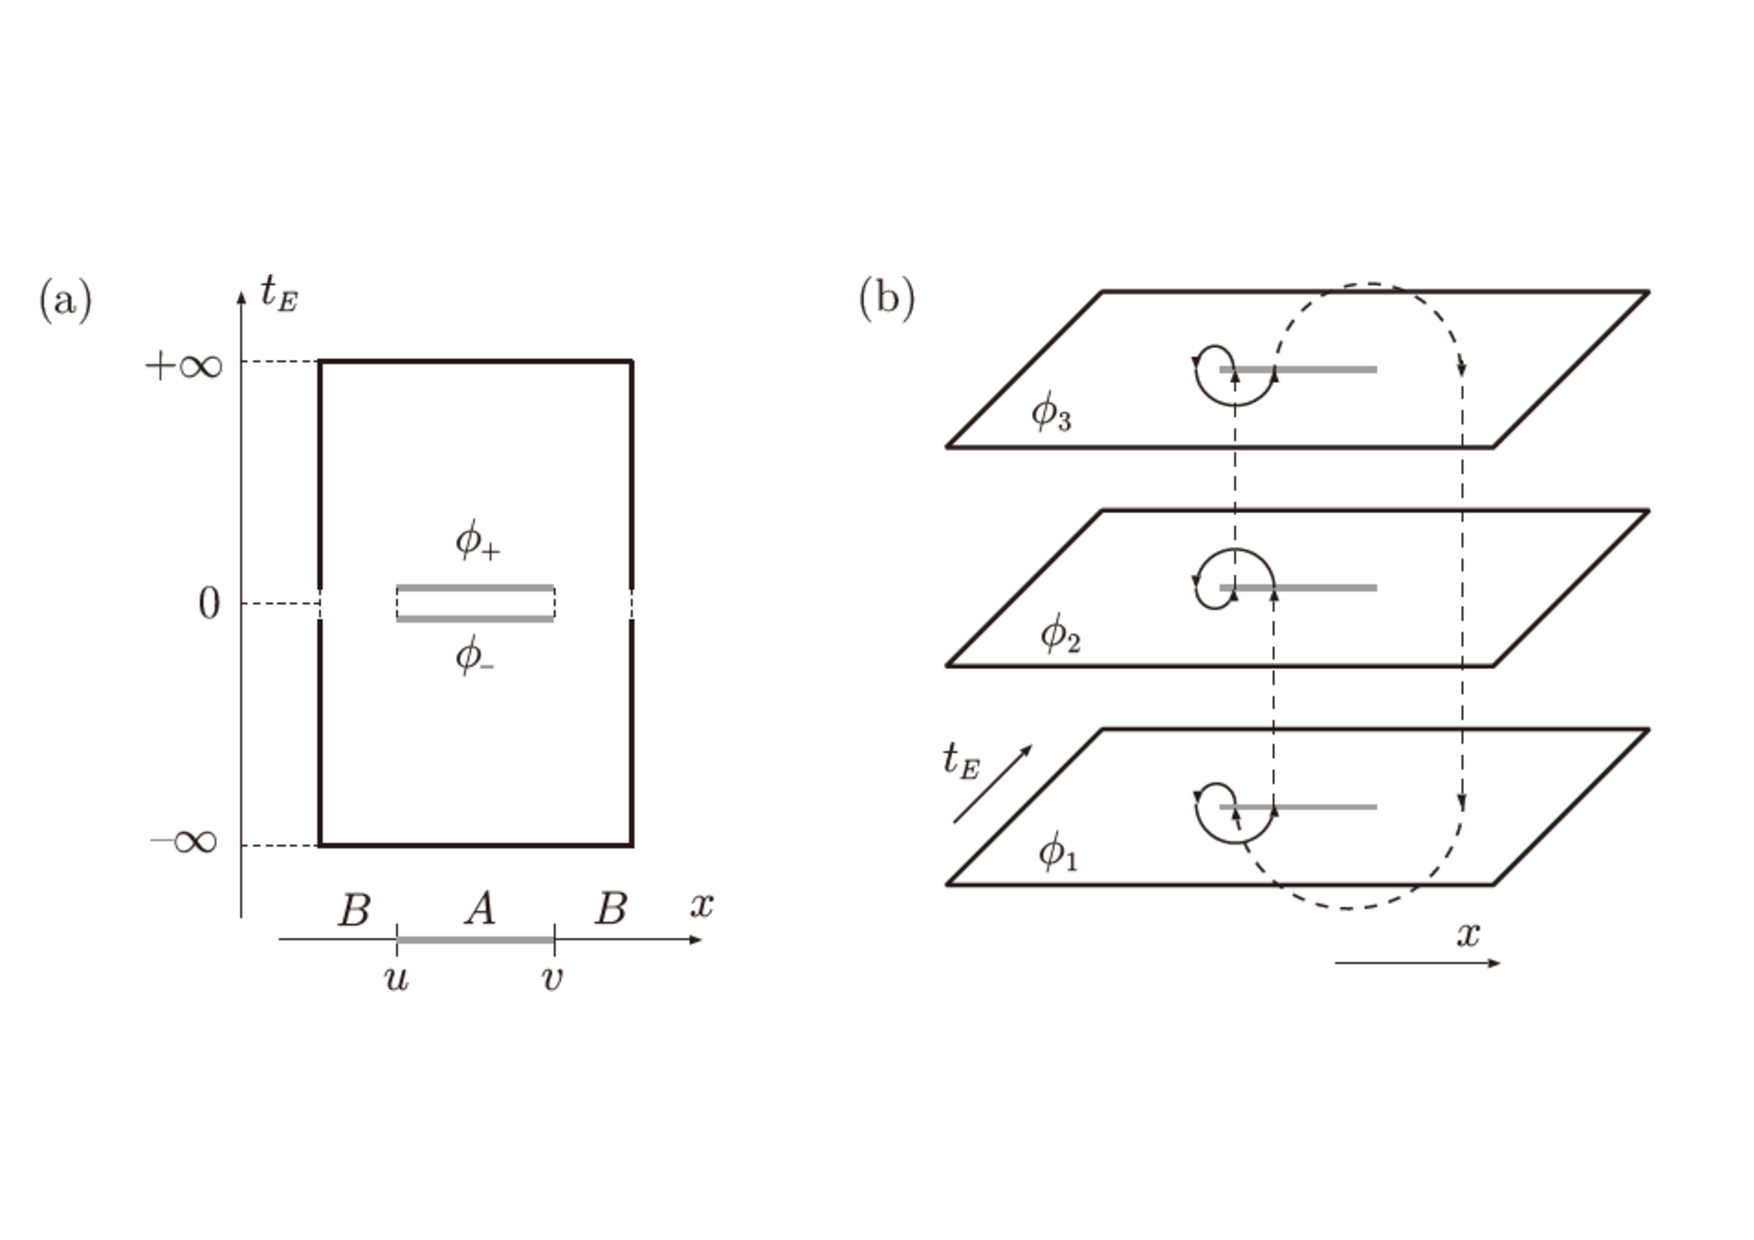
\includegraphics[width=7cm,angle=270]{replica.pdf}
     \caption{}
    \label{replica00}
\end{center}
\end{figure}

これらのことを求めると,$\mathrm{Tr}(\rho_A)^n$は,
\begin{align}
  \mathrm{Tr}\rho_{A}^{n}=&\biggl(\prod^{n}_{j}[D\phi_{j}]\biggr)[\rho_{A}]_{\phi_1\phi_2}[\rho_{A}]_{\phi_2\phi_3}+\cdots+[\rho_{A}]_{\phi_n\phi_1}\\
  -&\frac{1}{(Z_1)^n}\int_{\mathcal{R}_n}\mathcal{D}\phi e^{-\int dx_0dx_1\mathcal{L}^{n}}
\end{align}
と表すことができる.あとは,この値を計算することによって,領域Aにおけるエンタングルメントエントロピーを求めることができる.

\newpage

\subsubsection{Note}

\hrulefill

Q,Mの波動関数は$\phi(x)$で,これは位置$x$における情報しか持っていない.一方,場の理論の波動関数$\psi[\phi(x)]$は汎関数で表されて,初めから場全体の情報が含まれている(全ての$x$の情報).そのため場の理論の波動関数は,エンタングルメントなどの物理量を求める時に必要なdata setが初めから用意されていて,量子力学の時のように直積で後から加える必要がない.

\hrulefill

\subsubsection{エンタングルメントエントロピーの具体的な計算}
この節では,具体的なエンタングルメントエントロピーの計算を行う.簡単のために平坦な場のスカラー場について計算する.そこで,作用は,
\begin{align}
  S[\phi]=&\int dx_0d^dx\biggl[\frac{1}{2}(\partial_{x_0}\phi)^2+\frac{1}{2}(\partial_{x_1}\phi)^2+\frac{m^2}{2}\phi^2\biggr]\\
  =&\frac{1}{2}\int dx^{d+1}\phi(x)[\Delta+m^2]\phi(x)
\end{align}
部分積分を行った.
ここで,
\begin{align}
  \Delta=\partial_{x_0}^2+\partial_{x_1}^2
\end{align}
である.さらに,一般化されたガウスの法則,detとTrの関係
\begin{align}
  \int\frac{d^nx}{(2\pi)^{\frac{n}{2}}}\exp\biggl[-\frac{1}{2}\bvec{x}^{T}\bvec{M}\bvec{x}\biggr]=&\biggl[\mathrm{det}M\biggr]^{-\frac{1}{2}} \\
  \mathrm{det}M=&e^{\mathrm{Tr}\ln M}
\end{align}
を思いると,初めに分配関数について計算が進め得られる.
\begin{align}
  \label{logZ}
  Z=&\int\mathrm{D}\phi e^{-S}=e^{-\frac{1}{2}\mathrm{Tr}\log(\Delta+m^2)} \\
  \log Z=&-\frac{1}{2}V_{d+1}\int\frac{d^{d+1}k}{(2\pi)^{d+1}}\log[k^2+m^2]
\end{align}
さらに,schwinger parameterを用いて書き直すと,
\begin{empheqboxed}

  \begin{align}
    \frac{1}{A}=\int^{\infty}_{0}ds e^{-sA}
  \end{align}

\end{empheqboxed}
であるから,この両辺を$A$に関して積分した,
\begin{align}
  \log A=-\int^{\infty}_{0}\frac{ds}{s}e^{-sA}
\end{align}が使えて,(\ref{logZ})式の左辺の$\log$に適応すると,
\begin{align}
  \log Z=+\frac{V_{d+1}}{(2\pi)^{d+1}}\int \frac{ds}{s}\int d^{d+1}k e^{-s(m^2+k^2)}
\end{align}
を得る.ここで以前述べたreplica法を用いて,エンタングルメントエントロピーを計算する.巻きつけ作業していくつかのアンザツ後,$\mathrm{Tr}(\rho_A)^n$は,
\begin{align}
  \log\mathrm{Tr}(\rho_{A})^{n}=\frac{\pi}{6}(n-\frac{1}{n})V_{d-1}\int^{\infty}_{\epsilon^2}\frac{ds}{(4\pi s)^{\frac{d+1}{2}}}e^{-m^2s}
\end{align}
と求まる.したがって,(\ref{replica})式を用いてエンタングルメントエンタングルメントエントロピーは,
\begin{align}
  S_A=\frac{\pi}{3}V_{d-1}\int^{\infty}_{\epsilon^2}\frac{ds}{(4\pi s)^{\frac{d+1}{2}}}e^{-m^2s}
\end{align}
を得る,この結果から明らかなように.運動量カットオフの紫外極限をとるとこのエンタングルメントエントロピーは発散する.このエンタングルメントエントロピーをさらに計算するために.指数のところをテイラー展開にしてその振る舞いを確かめる,
\begin{align}
  e^{-m^2s}=\sum_{n=0}^{\infty}\frac{1}{n!}(-m^2s)^n
\end{align}
を用いると,積分はさらに計算できる.ここでは,あとで確認する4次元$d=3$についてその積分を計算する.
\begin{align}
  S_{A,d=3}=&\frac{\pi}{3}\frac{V_{2}}{(4\pi)^2}\int^{\infty}_{\epsilon^2}ds s^{-2}(\underbrace{1-m^2s}_{UV-divergence}+\underbrace{m^4s^2+\cdots}_{UV-finite})
\end{align}
である,紫外発散する部分とそれ以外の部分に分ければ,
\begin{align}
  S_{UV-divergent}=\frac{\pi}{3}\frac{V_{2}}{(4\pi)^2}\biggl(\frac{1}{\epsilon^2}+2m^2\log\epsilon \biggr)
\end{align}
が紫外発散する部分で,紫外発散しない部分もIRの発散が残る,そこで,十分大きな値$N\to \infty$を用いて,UV-finite部分を書き出せば,
\begin{align}
  S_{UV-finite}=\frac{\pi}{3}\frac{V_{2}}{(4\pi)^2}\biggl(-\frac{1}{N}-m^2\log N+m^2N+\mbox{UV-finite part}\biggr)
\end{align}
となる.第一項は,$N\to\infty$の極限で$0$になる.この式から$\log$発散と整関数の最低次の発散は一次関数で効いてくることがわかった.この結果は,あとで用いる.

\chapter{Entanglement Entropy in de Sitter space}

\begin{comment}
  \section{Euclidean vacuum mode functions for a scalar field on open de Sitter space\cite{10}}

  低密度で負の曲率宇宙を予測するoneバブルのinflationalな宇宙シナリオの最近の研究によって動機づけられ、双曲線タイムスライスによって構成されるドジッター時空のopen chartにおけるのスカラー場のユークリッド真空モード関数を調べる。

  初期の状態のすべての情報を失うほど、初期のinflation時代が長過ぎてはならないので、open inflationalな宇宙の可能性を考えるとき,インフレーションを引き起こすためのinflaton場の量子揺らぎの初期条件に関する問題に直面する.

  false真空の量子減衰によって,指数関数的に拡大するfalse真空宇宙でオープンな宇宙が生成されるワンバブルのシナリオでは、初期状態はドジッター不変のユークリッド真空は正当化される。ここでは、ユークリッドの真空モード関数とは、任意の質量と曲率結合を持つスカラー場のオープンチャートに関して示す。

  興味深いことに、無次元masslessのコンフォーマルスカラーに対応する臨界値よりも小さな有効質量を持つスカラー場のために、オープンチャートの時間一定面の超曲面上で平方積分可能ではない離散モードのセットが現れる
  \subsection{Introduction}
  最近の観測結果からわかることは,宇宙の曲率は,負極率であることが示唆されている,一つのConsistentなpen宇宙の出現のシナリオに,擬真空が支配的な宇宙の加速度膨張が上げられる.このideaは,Gottによって初めて提唱された.\cite{11}スタンダードなinflationシナリオの枠組みでは,horizon問題は,空間の急激な膨張によって解決される.平坦チャートの晴れる大きさは,はじめhorizon程度の大きさだあったが,宇宙の急激の膨張で膨張し,現在のわれわのhorizonサイズは,その平坦チャートの中にいることで平坦性問題がhorizon問題と同時に解決された.したがって,現在の我々のいる宇宙の曲率は,必然的に膨張とともに減少していくことになる,これは,open universeを考える上で問題になる,
  一方,擬真空においてde Sitter時空で記述されるバブルが生成されたと考えると,トンネル効果によってEuclidianな対称性O(4)を持つ時空から生成されるのでO(3,1)対称性を持つことになる,この時,ユークリッド時空なので因果関係などはなくhorizon問題は,解決される,

  \textcolor{red}{O(4)とかO(3,1)あたりがわかっていない
  de Sitter時空にO(3,1)があるのか,de Sitteとは何か.つまり,Minkowsikiとどう違うのか.
  メトリックは違うが,対称性に関しては同じ感じがするが}

  もし,バブル生成が起こってから,真空のエネルギーが宇宙のエネルギーのうちう優勢な要素に永遠にならなければ,曲率のエネルギーがずっと優勢になり,観測されているようにFRW universeが結論付ける,\textcolor{red}{ここら変の議論が実際にペンを動かして確かめる必要がる,}Bigbangやそれに伴うhotなeraが実現されない.そうすると,エントロピーが生成される過程が生まれないために,Entropy Problem\footnote{There exists the 'entropy problem' of the early universe, that is, why did the universe begin with an extremely low entropy and how did it evolve into such high entropy at late times? }が解決されないことになる,そこで,secondary inflationがバブル内で起きることを要求する.このモデルが,スタンダードなinflationシナリオと本質的に異なるポイントは,secondary inflation開始時の曲率程度のスケールのhorizonサイズのpatchが,現在の我々のhorizonサイズよりはるかに大きくならない可能性がある,

   これは、secondary inflationの開始時の宇宙の量子状態の記憶は消去されず、観測された大規模な温度と密度の変動に直接影響を与えることを意味することになる,\textcolor{red}{ここら辺の量子状態の記録が消える消えないの議論がわからない,また,なぜpatchの大きさがそれに関係し,そのスケールが曲率のスケールくらいなどと予測されているのか.仮説としては,secondary inflationの場合は,宇宙の膨張が抑えられて,現在観測している我々のデータに,secondary inflation前の量子状態が影響するという意味なのかなって感じ.}

   したがって,我々は,バブル内のsecondary inflation時におけるinflaton場について色々と調べる必要が出てくる.これに関する先行研究は,様々に行われていて,O(4)におけるトンネリング効果に関する公式などが開発された.これまでの研究はすべて、一般的な状況に実際に適用可能な量子状態を調べる技術はまだないという意味ではかなり正式なレベルにとどまっていた.(rather practical level to general situations)

  しかし,それは,拡張され\cite{12},この論文ではさらに重力を入れて考え他場合について議論する.

  第1のステップとして、重力のバックグラウンド反応が無視され、バックグラウンドメトリックがde Sitter空間に固定される場合を考える。次に、bubble内部の時空は、空間が開いているde Sitter空間のチャートによって記述され、inflaton場は、空間的に開いた時間スライスの超曲面で一定の値をとる。さらに、バブル核形成を引き起こすトンネル場がinflaton場$\phi$と相互作用しない場合、$\phi$の量子状態はトンネリングプロセスの影響を全く受けない。次に、トンネリング前の$\phi$の量子状態がユークリッド真空であることを前提とする。これは先の擬真空膨張が十分に長く続く場合には良い近似であるはずであるが、bubble内部の量子状態はそのままである。そこで,de Sitter空間のオープンチャートでモード関数によって量子状態を記述する必要があります。openチャートでユークリッド真空モード関数を得る方法が分かったら、トンネルを起こす場との結合によって$\phi$の質量が時間的に変化する場合や幾何が後の段階で正確なde Sitter空間から逸脱した場合に拡張するのはかなり簡単にになる,

  ちなみに,de Sitterの場合でもflat chartとclosed chartでは先行研究がある, \cite{13}とかT.S.
  Bunch and P.C. Davies, Proc. R. Soc. London, Ser. A 60, 117 (1978), B. Allen, Phys. Rev. D 37, 2078 (1988).
\end{comment}




\section{Set Up}
\textcolor{red}{もう一度構成から書き直しをする.足りないところは手書きノート見ながら埋める.}
この章では,まず,これからどのような設定でエンタングルメントエントロピーを求めるかを決め,そのエンタングルメントエントロピーをどのようなステップで求めるかを述べる.

我々の目標は,de Sitter時空での自由スカラー場の真空の大局的な相関\footnote{エンタングルメントエントロピーは,大局的な相関である.普段CMBなどで考えている相関は,局所的な複数の点の壮観である.エンタングルメントエントロピーの相関は,領域同士の相関である.}を求めることである.この真空の相関は,宇宙が膨張する時に生じたものである.de Sitter時空を考える理由は,初期宇宙がde Sitter時空に近似できることから初期宇宙で生じたエンタングルメントエントロピーを評価するのに適しているからである.
\subsubsection{de Sitter時空におけるevent Horizon}
今,時刻$t=0$に$x=0$地点にいるObserverを考える,宇宙が膨張しているので,十分遠方からの光は観測できないと推測される.そこで,このObserverに届く情報はObserverからどの距離までにあるのかについて求める.情報が届かなくなる境界のことをよくEvent Horizonと呼ぶ.宇宙の中で最速なのは光であるので,光が無限の未来にObserverに到達するような場合、光源がはじめに放出された時刻における、観測者と光源の放出された場所までの距離がちょうどEvent Horizonと呼ばれる境界となる。時刻$t^{\prime}$に光源をでた光が、Observerに到達したとすると、その光源までの距離は,
\begin{align}
  l_{ds}&=a(t^{\prime})\int_{null}|d\bvec{x}|\\
  &=a(t^{\prime})\int^{\infty}_{t^{\prime}}\frac{dt}{a(t)}
\end{align}
となる,1行目から二行目の変形は,nullは$|d\bvec{x}|=d\eta=\dfrac{dt}{a(t)}$であることを用いた.de Sitter時空のOpen Chartのメトリックは
\begin{align}
ds^2=dt^2-e^{2H_{dS}t}d\bvec{x}^2
\end{align}
で表せるので,$a(t)=e^{H_{dS}}$である.ゆえに,積分した結果は、
\begin{align}
l_{dS}=\frac{1}{H_{dS}}
\end{align}
となる.この結果からわかることは、de Sitter時空におけるEvent Horizonは一定であり、宇宙膨張によって広がらないということでる。以降の議論のために、共動座標についてもここで確認しておく。座標$x$は、共動座標と呼ばれこの尺度で一定な長さでも、宇宙膨張によって実際の物理的な長さは引き延ばされる。($\sum x_i^2 = R^2$ は宇宙膨張とともに拡大する球である。)一方、$a(t)x_i$で書かれた座標系は、物理的な座標であり、この座標系で一定の長さは、物理的な実際の長さが常に一定である。

$dt=e^{H_{ds}t}d\eta$を用いてconformal time$\eta$を導入する.すると,
\begin{align}
\eta=-\frac{e^{-H_{ds}t}}{H_{ds}}
\end{align}
であるので,
\begin{align}
e^{-H_{ds}t}=-H_{ds}\eta
\end{align}
を用いると,メトリックはもっと簡単に,
\begin{align}
ds^2=\frac{1}{(H_{ds}\eta)^2}(-d\eta^2+dx^2+dy^2+dz^2)
\end{align}

\section{de Sitter時空の対称性}
4次元de Sitter時空は5次元Minkowski時空,
\begin{align}
  \label{EDS}
  ds^2_{5}=-dX_0^2+dX^2_{1}+dX^2_{2}+dX^2_{3}+dX^2_{4}
\end{align}
に埋め込まれた双曲面,
\begin{align}
  +X_0^2-X_1^2-X_2^2-X_3^2-X_4^2=R_{ds}^2=H^{-2}
\end{align}
によって表現される.この埋め込みによって得られるde Sitter時空のFlat Chartは,
新しい座標系($\tau,x_{i}$)を用意することで実現される.新旧の座標の関係は,次で与える.
\begin{align}
  X_{0}=&\frac{1}{2H}(H\eta-\frac{1}{H\eta})-\frac{1}{2}\frac{x_i^2}{\eta}\\
  X_{i}=&\frac{x_i}{H\eta}\\
  X_{4}=&-\frac{1}{2H}(H\eta+\frac{1}{H\eta})+\frac{1}{2}\frac{x_i^2}{\eta}
\end{align}
ただし,先にも述べたように$\eta<0$である.
この変換の下で,メトリック(\ref{EDS})式は,
\begin{align}
  ds^{2}=\frac{1}{H^2\eta^2}(-d\eta^2+dx_{i}^2)
\end{align}
と,Flat chartのメトリックになる,ここで,このchartが覆っている領域は,上の対応関係から,$X_{0}+X_{4}=-\frac{1}{2H^2\eta}>0$であるので,図\ref{vchart}のFlat Chartのように全体の斜め半分のみを覆うことがわかる.ここで,$\eta\to 0$の極限では,この座標の対応は,
\begin{align}
  X_{0}=&-\frac{1}{2H^2\eta}-\frac{1}{2}\frac{x_i^2}{\eta}\\
  X_{i}=&\frac{x_i}{H\eta}\\
  X_{4}=&-\frac{1}{2H^2\eta}+\frac{1}{2}\frac{x_i^2}{\eta}
\end{align}
となり,これは近似的に,
\begin{align}
  -X_{0}^2+X_{i}^2+X_{4}^2=0
\end{align}
満たす.すなわち,$\eta\to0$の極限では,時空は近似的に,
\begin{align}
  X_{A}\to\lambda X_{A}
\end{align}
のscale変換の下で不変である.今,$X_{A}$は,$\frac{1}{\eta}$の一次関数で関数であらわせれているから,
このこの対称性から,$\eta$がrescalingできることになる.さらに,エントロピーを評価する$\eta=$一定面上でのメトリックは,
\begin{align}
  ds^2_{\eta\to0}=\frac{dx^2_{i}}{H^2\eta^2}
\end{align}
となるので,時空は,$\eta\to\lambda\eta$と同時に$x_{i}\to\lambda x_{i}$とする変換の下でも不変である.
\begin{itemize}
  \item{時空は,$\eta\to\lambda\eta$とする変換の下でも不変}
  \item{時空は,$\eta\to\lambda\eta$と同時に$x_{i}\to\lambda x_{i}$とする変換の下で不変}
\end{itemize}
以上のことから,$\eta\to0$の極限では,時空に$x_{i}\to\lambda x_{i}$の変換の下での対称性があることがわかる.したがって,de Sitter時空におけるエンタングルメントエントロピーにおける時間に依存しないLong-ange部分は,この空間方向のリスケールによって不変である.すなわち,Entangle Surfaceはこのcomformal trasformationでGlobal chart(Flat chart)における時間一定面のSlice($S^3$)のちょうど真ん中の$S^2$面になるように取ることができる.この事実から,我々は,Open ChartにおけるR,L領域とentangle serfaceの中と外を対応付けられる.
そこで,これ以降は,Flat chartにおけるEntangle Surfaceの中と外の相関を求めるために,Open chartのR,L領域のエンタングルメントについて考える.さらに,Open chartのR,L領域のエンタングルメントについて考えるために,de Sitter時空におけるOpen chartの場の理論について勉強する必要がある.


  \begin{figure}[H]
    \begin{center}
    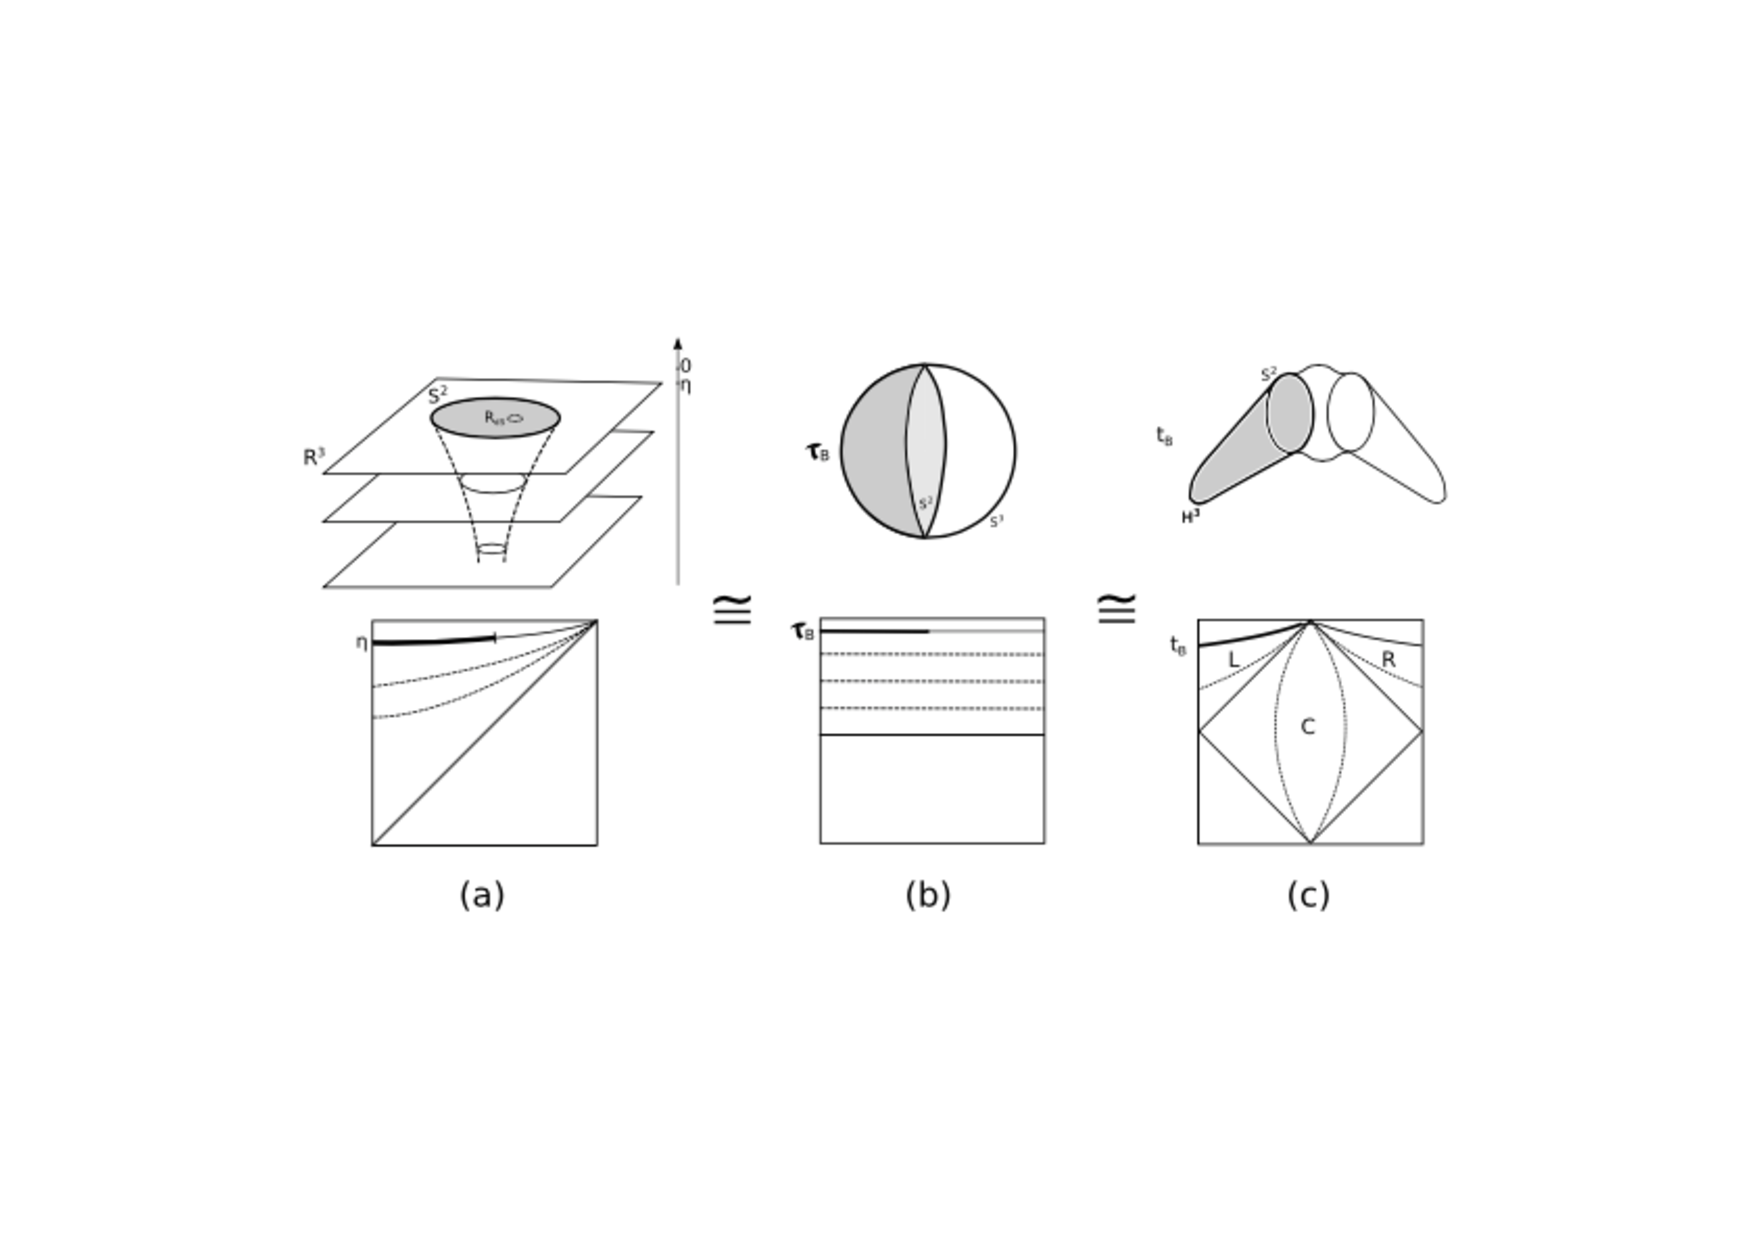
\includegraphics[width=8cm,angle=270]{de.pdf}
    \caption{title}
    \end{center}
  \end{figure}

  \begin{figure}[H]
    \begin{center}
    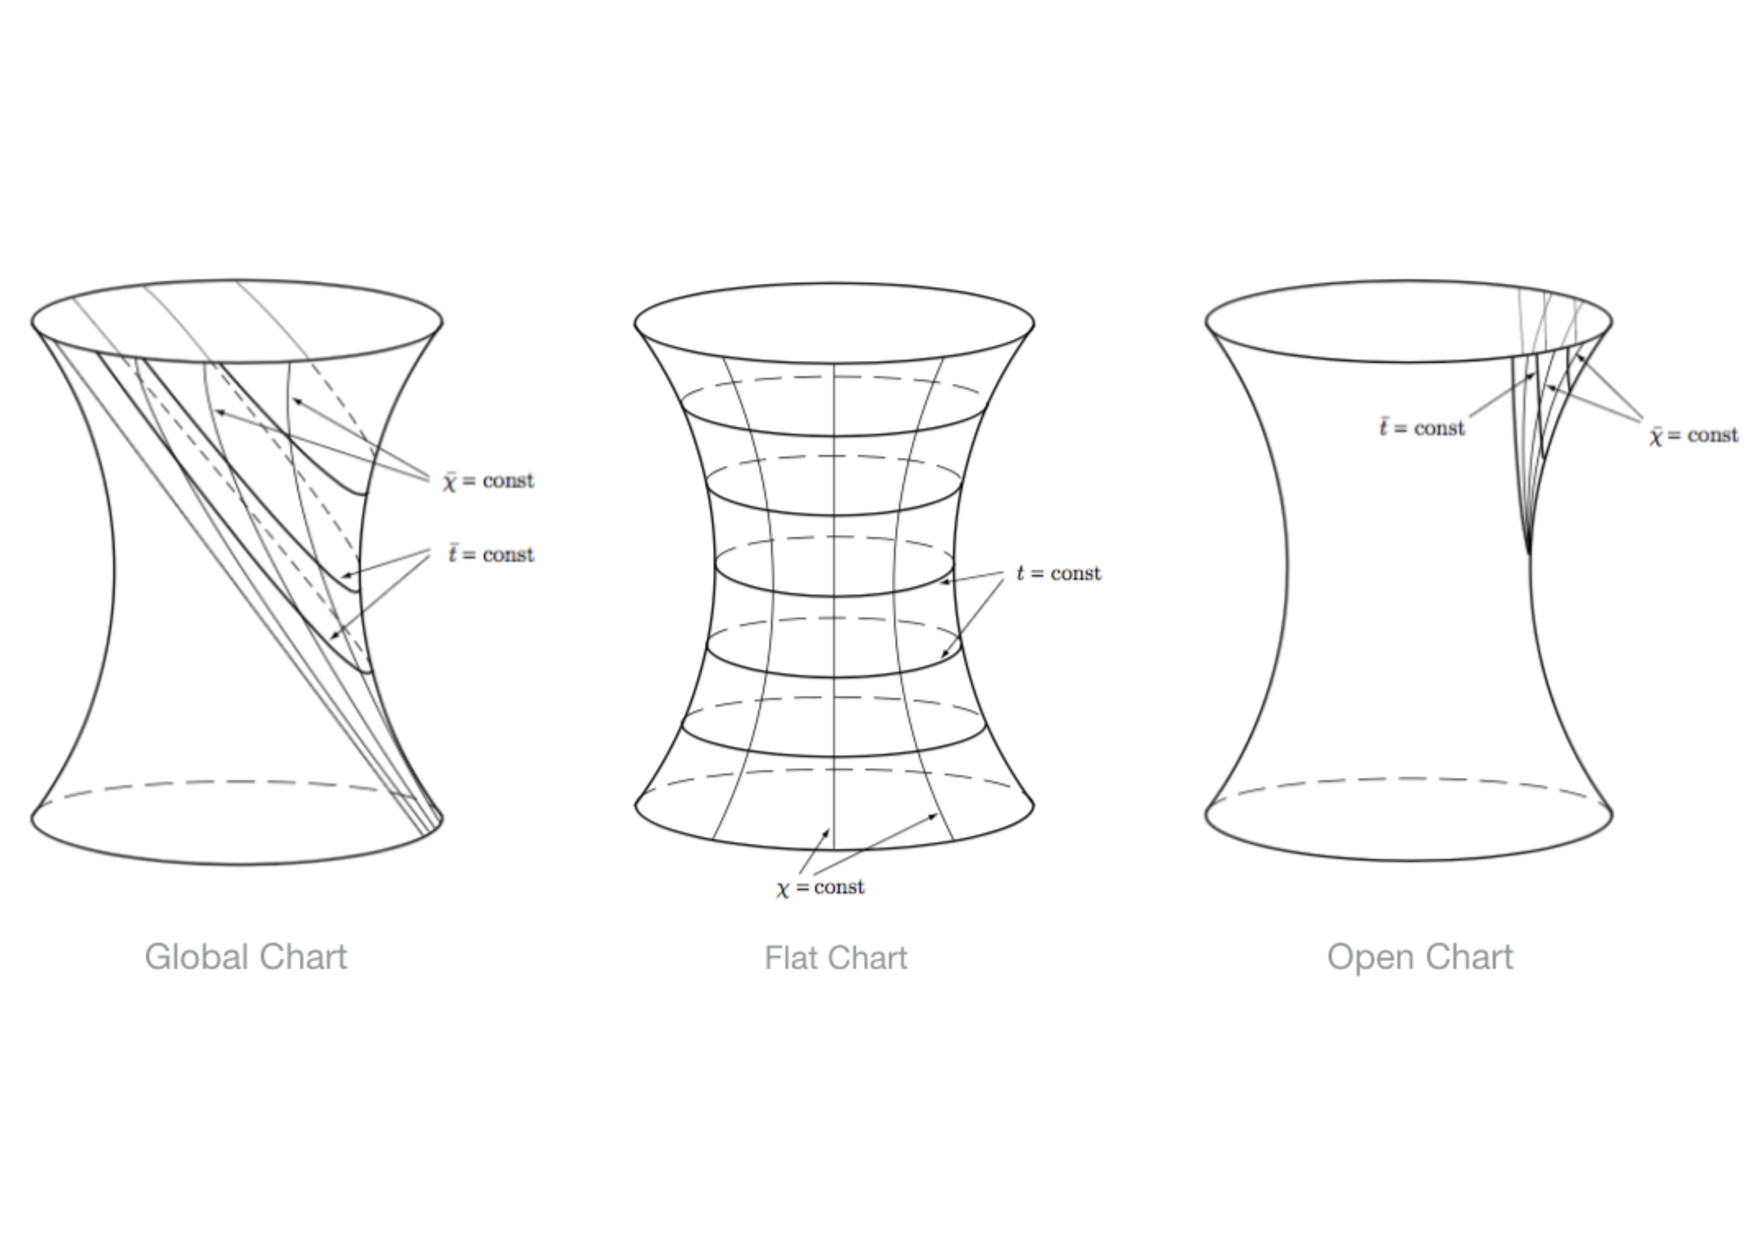
\includegraphics[width=7.5cm,angle=270]{Web.pdf}
    \caption{de Sitter spaceの様々なChat}
    \label{vchart}
    \end{center}
  \end{figure}

\section{Scalar Field on Open de Sitter Space}
ここでは,de Sitter時空のopen chartでのスカラー場のモード展開に浮いて議論する,
まずはじめに,あとで波動関数の規格化を行う際に,R,L,C領域がそれぞれどのような関係性になっているかについて知る必要がある.(具体的には,解析接続で繋がっていることを用いて,de Sitter space全体に渡ってCauchy surfaceを定義して規格化を行う.)
\subsubsection{Global Chart}
\textcolor{red}{まずはじめにFlat chartのメトリックがどのような形をしているのかそれぞれの領域のメトリックを見せる.次にそのメトリックがきちんとEdSから得られることを確認する.}
de Sitter時空は,5次元Minkowski spacetimeに埋め込まれた4次元部分空間である双曲面として定義される,5次元Minkowski時空の座標を$(x_0,x_1,x_2,x_3,x_4)$で表すと,その計量は,
\begin{equation}
  ds^2=-dx_0^2+dx_1^2+dx_2^2+dx_3^2+dx_4^2
\end{equation}
となる,また,この時空に埋め込まれた双曲面は,半径を$H^{-1}$とすれば,
\begin{equation}
  \label{1.2}
  -x_0^2+x_1^2+x_2^2+x_3^2+x_4^2=H^{-2}
\end{equation}
で定義される.
今,
\begin{eqnarray}
  x_0&=&H^{-1}\sinh{t} \\
  x_1&=&H^{-1}\cosh{t}\cos{\chi} \\
  x_2&=&H^{-1}\cosh{t}\sin{\chi}cos{\theta} \\
  x_3&=&H^{-1}\cosh{t}\sin{\chi}\sin{\theta}\cos{\phi} \\
  x_4&=&H^{-1}\cosh{t}\sin{\chi}\sin{\theta}\sin{\phi} \\
\end{eqnarray}
によって新しい座標系$(t,\chi,\theta,\phi)$を導入すると,この座標系でのMinkowski計量は,
\begin{eqnarray}
  ds^2=H^{-2}\biggr[-dt^2+\cosh^2{t}(d\chi^2+\sin^2\chi(d\theta^2+\sin^2\theta d\phi^2))\biggr]
\end{eqnarray}
となる.ただし,それぞれのパレメータの取りうる範囲は,
\begin{eqnarray}
  -\infty< t < \infty,\hspace{0.5cm} 0 \leqslant \chi \leqslant \pi,\hspace{0.5cm} 0 \leqslant \theta \leqslant \pi, \hspace{0.5cm} 0 \leqslant \phi \leqslant 2\pi
\end{eqnarray}である.また,$d\theta^2+\sin^2\theta d\phi^2$の部分は,よく$d\Omega_2^2$という表記で省略されることが多い,
このとき,$\chi=0,\pi$と$\theta=0,\pi$に特異点がある.このチャートは,de Sitter時空の全体を覆っているので,Global Chartと呼ばれる,
\begin{figure}[H]
\begin{center}
  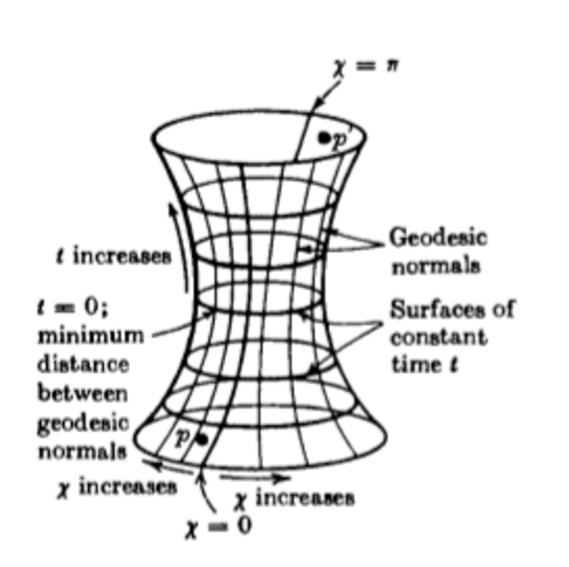
\includegraphics[width=5cm,angle=0]{deSitter.pdf}
     \caption{}
    \label{desitter}
\end{center}
\end{figure}
\subsubsection{Open Chart}
次に,この章で大切になるOpen Chartについて学ぶ,Open Chartは,(\ref{1.2})式で,座標変換$(t,r,\theta,\phi)$を
\begin{eqnarray}
  x_0&=&H^{-1}\sinh{t}\cosh{r} \\
  x_1&=&H^{-1}\cosh{t} \geqslant H^{-1} \\
  x_2&=&H^{-1}\sinh{t}\sinh{r}\cos{\theta} \\
  x_3&=&H^{-1}\sinh{t}\sinh{r}\sin{\theta}\cos{\phi} \\
  x_4&=&H^{-1}\sinh{t}\sinh{r}\sin{\theta}\sin{\phi} \\
\end{eqnarray}
によって座標系を導入した場合のChartである.このChartにおける計量は,
\begin{eqnarray}
\label{openM}
      ds^2=H^{-2}\biggr[-dt^2+\sinh^2{t}(dr^2+\sinh^2r(d\theta^2+\sin^2\theta d\phi^2))\biggr]
\end{eqnarray}
となる,ここで,$dr^2+\sinh^2r(d\theta^2+\sin^2\theta d\phi^2)$の部分は,よく$dH_3^2$という表記で省略されることが多い,

中央部分ののChartの張り方,
\begin{align}
  \label{1.19}
  x_0&=H^{-1}\cos{t}\sinh{r} \\
  \label{test}
  x_1&=-H^{-1}\sin{t} \\
  x_2&=H^{-1}\cos{t}\cosh{r}\cos{\theta} \\
  x_3&=H^{-1}\cos{t}\cosh{r}\sin{\theta}\cos{\phi} \\
  x_4&=H^{-1}\cos{t}\cosh{r}\sin{\theta}\sin{\phi} \\
\end{align}
を導入することで,得られる,ここで$x_1$は三角関数のみで表せれるので,取りうる値が制限されて,
\begin{align}
  -H^{-1} \leqslant x_1 \leqslant H^{-1}
\end{align}
であることから,このChartは確かに,中央の部分しか覆っていない,また,途中でChartが途切れているように見えるが,はじめのGlobal Chartで見たように,角度部分には重複があり左回りと右回りでは,どちらも$t$が増加する向きである.この座標系を導入すると,(\ref{1.2})式は,
\begin{align}
\label{CenterM}
  ds^2=H^{-2}\biggl[dt^2+\cos^2t(-dr^2+\cosh^2r(d\theta^2+d\phi^2\sin^2\theta))\biggr]
\end{align}
となる.中央部分のチャートは、他のチャートと異なり時間座標と空間座標の役割が異なっていることに注意する。

\subsection{Euclidean de Siiter space}
Euclidean de Sitter Spaceとは,5次元Euclid空間に埋め込めこまれた4次元球である,その超曲面は,
\begin{eqnarray}
  \tilde{x}_0^2+x_1^2+x_2^2+x_3^2+x_4^2=H^{-2}
\end{eqnarray}
で定義できる.この超曲面場での座標系は,次のように張ることができる.
\begin{eqnarray}
  \label{1.19}
  \tilde{x}_0&=&H^{-1}\cos{\tau}\cos{\rho} \\
  \label{test}
  x_1&=&H^{-1}\sin{\tau} \\
  x_2&=&H^{-1}\cos{\tau}\sin{\rho}\cos{\theta} \\
  x_3&=&H^{-1}\cos{\tau}\sin{\rho}\sin{\theta}\cos{\phi} \\
  x_4&=&H^{-1}\cos{\tau}\sin{\rho}\sin{\theta}\sin{\phi} \\
\end{eqnarray}
ただし,
\begin{eqnarray}
  \label{1.25}
  -\frac{\pi}{2} \leqslant \tau \leqslant \frac{\pi}{2},\hspace{0.5cm} 0 \leqslant \rho \leqslant \pi,\hspace{0.5cm} 0 \leqslant \theta \leqslant \pi, \hspace{0.5cm} 0 \leqslant \phi \leqslant 2\pi
\end{eqnarray}
である.5次元Eclide空間における計量は,
\begin{eqnarray}
  ds_{E}^2=d{\tilde{x}_0}^2+dx_1^2+dx_2^2+dx_3^2+dx_4^2
\end{eqnarray}
 なので,この超曲面の計量は,
 \begin{eqnarray}
   \label{4sphereM}
   {ds_{E}}^2=H^{-2}\biggl[d\tau^2 + \cos^2\tau(d\rho^2+\sin^2\rho d\Omega^2)\biggr]
 \end{eqnarray}
 という形になる.次に,この時空において,$\tilde{x}_0\rightarrow ix_{0}$のwickローテーション(analytic continuation)を行う.この操作で,多様体は3つのLorentz多様体に分けることができる.この操作について詳しくみていくことにする.(\ref{1.19})式を見れば,
 \begin{eqnarray}
   ix_0=\cos\tau\cos\rho
 \end{eqnarray}
を満たすことになる.今,座標$x_0$は,Real numberなので,左辺はimaginary numberとなることがわかる.一方,$\tau$と$\rho$が独立な変数であることに注意する\footnote{$\cos=a+ib,\cos\rho=c+id$とおいた時に,これらの積がpure imaginaryになるのは$ac-bd=0$の時である,しかし,このように$a,b,c,d$を取ると$\tau$と$\rho$が独立で無くなる},$x_0$がrealになるためには,次の2パターンが考えられる.
\begin{center}
  (i)\ $\cos\tau$がrealで$\cos\rho$がpure imaginary \\
  (ii)\ $\cos\tau$がpure imaginaryで$\cos\rho$がreal
\end{center}

それぞれの場合について,metric(\ref{4sphereM})がどのようにwick rotationされるかを考える.
ただし,三角関数と双曲線関数の関係,
\begin{eqnarray}
  \label{1.29}
  \sin{i\theta}=i\sinh{\theta} \\
  \label{1.30}
    \cos{i\theta}=\cosh{\theta}
\end{eqnarray}
と,$\rho,\tau$のwick rotationで他の変数$x_1\sim x_4$がImaginary numberにならないようにすることに注意する.
\subsubsection{(i)}
$\cos\tau$がrealとなることから$\tau$は,realまたはimaginalのどちらかである,もし,Imaginary numberであれば,加法定理で分解した時に$\sin$の因子からimaginary numberが出てくる.また,$\tau$がpure imaginalであれば,$x_2\sim x_4$が(\ref{1.29})式からimaginary numberとなるので不適.従って,$\tau$はreal numberであれば良いことがわかった.次に$\sin\rho$がimaginary numberになるには,
\begin{eqnarray}
  \rho=\pm ir+\frac{\pi}{2}
\end{eqnarray}
と取ればいい.ただし,$\rho$の実部の取りうる範囲(\ref{1.25})に注意した.

以上より,(i)の場合は,
\begin{align}
  \tau&=t_{C} \\
  \rho &= \pm ir_{C} +\frac{\pi}{2}
\end{align}
というようにwick rotationすればいいことがわかる.
これを,$r_{C},t_{C}$についてとくと,
\begin{align}
  t_{C} = \tau& &(-\frac{\pi}{2} \leqslant t_{c} \leqslant \frac{\pi}{2}) \\
  r_{C} =i(\rho-\frac{\pi}{2})& &(-\infty \leqslant r \leqslant \infty)
\end{align}
となる,ただし,$\rho$の係数の符号は,$x_0$が正の値になるように,定めた.
この変換の下で,メトリック(\ref{4sphereM})式は,
\begin{align}
  ds^2=H^{-2}\biggl[{dt_{C}}^2+\cos^2t_{C}(-{dr_{C}}^2+\cosh^2r_{C}d\Omega^2) \biggr]
\end{align}
となる.これはちょうどde Sitter時空の中央をおおうChart(\ref{CenterM})式に一致する.
\subsubsection{(ii)}
次に,$\cos\tau$がpure imaginaryで$\cos\rho$がrealである場合について考える.
$\tau$は,次の場合にが考えられる.
\begin{align}
  \tau=it\pm\frac{\pi}{2},-it\pm\frac{\pi}{2}
\end{align}
ただし,real partが$\frac{\pi}{2}$となるように選んだ理由は,$\tau$の変域とpure imaginaryになるようにするためである。(4つの候補がある理由は、open chartに4箇所の端があるからである。chartの上側のR領域とL領域、chartの下側のR領域L領域である。) $\cos\tau$がimaginary numberであるとき,$\sin\rho$がrealであれば,$x_2 \sim x_4$がimaginary numberとなるので,$\rho$は$\sin\rho$がpure imaginaryかつ,$\cos\tau$が仮定からrealになるように取ればいい.その候補として,
\begin{align}
  \rho=\pm ir
\end{align}
が考えられる.先ほど同様に,$x_0$が正の値になるようにこれらの値を定めると,
\begin{align}
  \label{1.47}
  \tau&=it-\frac{\pi}{2},-it+\frac{\pi}{2} \\
  \label{1.48}
  \rho &= \pm ir
\end{align}
まで絞られる.\footnote{wick rotationした後の$x_0$は,(\ref{1.47})を代入すると,$x_0=\cosh{r}\sinh{t}$となるが,$t \geqslant 0$に制限すれば,この値は常に正の値になる.}一方,$\rho$の符号の不定性は,$x_2\sim x_4$が正負どちらの値も取りうるので,$x_0$の場合と異なりどちらでも良いが,ここでは$x_2\sim x_4$の係数$\cos\tau\sin\rho$がはじめ正の値になるように定めると,
\begin{align}
  \cos\tau\sin\rho&=\cos(+it-\frac{\pi}{2})\sin(\pm ir) \\
  &=i(\pm i)\sinh{t}\sinh{r}
\end{align}
となるので,$\rho=-ir$と選べば良いことになる.以上より,(ii)の場合では,
\begin{align}
  \label{1.49}
  \tau&=it_{L}-\frac{\pi}{2},-it_{R}+\frac{\pi}{2} \\
  \label{1.59}
  \rho&=-ir
\end{align}
すなわち,
\begin{align}
  t_{R}&=i(\tau-\frac{\pi}{2})& &(t_{R} \geqslant 0) \\
  r_{R}&=i\rho& &(r_{R} \geqslant 0) \\
  t_{L}&=-i(\tau+\frac{\pi}{2})& &(t_{L} \geqslant 0) \\
  r_{L}&=i\rho& &(r_{L} \geqslant 0)
\end{align}
と定めれば良いことがわかる,
また,このような変換の元で,超曲面のメトリック(\ref{4sphereM})は,それぞれ,
\begin{align}
  ds^2&=H^{-2}\biggr[-dt_{R}^2+\sinh^2{t_{R}}(dr_{R}^2+\sinh^2r_{R}(d\theta^2+\sin^2\theta d\phi^2))\biggr] \\
ds^2&=H^{-2}\biggr[-dt_{L}^2+\sinh^2{t_{R}}(dr_{L}^2+\sinh^2r_{L}(d\theta^2+\sin^2\theta d\phi^2))\biggr]
\end{align}
のようになる,これらは,(\ref{openM})式で表されるOpen Chartのメトリックに一致する.また,ここでは,$\tau$の実部として$\frac{\pi}{2}$を選んだものを$R$側のChart,$-\frac{\pi}{2}$を選んだものを$L$側のChartとしている.

以上より,5次元Euclid時空に埋め込まれた,4次元球の超曲面が作る時空において第$0$成分をwick rotationすることで時空は,3つのopen chart($R,L,C$)に対応するde Sitter時空に分けられるということが結論づけられた.上の変換では,$\rho$と$\tau$をreal numberからcomplex numberへ拡張したので,単純に変数の自由度が増えているように見えるが実際は,増えていない.実際,(\ref{1.47})式では,$\tau$のreal partは,RとL領域で一意に$\pm\frac{\pi}{2}$に決まっている.また,(\ref{1.48})式に関しても,$r$は,real numberなので$\rho$はpure imaginaryで自由度が変わっていない.(\ref{1.49}),(\ref{1.50})式に関しても同様である.

最後に,R領域とL領域につながりについて考える.上で議論したように,RとLは,$\tau$が$(-\frac{\pi}{2},\frac{\pi}{2})$で変換するようなpathによって繋がっている.この時,pathとして上の議論では$x_0$が正になるようなpathについて今回は考えたが,逆の半球に関するpathでも繋がっている.(例えば,図\ref{desRL}のちょうど真ん中の線は,右のL領域の$(\rho=0,-\tau=\frac{\pi}{2})$から始まり,$(\rho=\frac{\pi}{2},-\tau=\frac{\pi}{2}\sim\frac{\pi}{2})$のCの領域を通過して,$(\rho=0,\tau=\frac{\pi}{2})$の左側R領域に到達するpathで繋がっている.)
また,中央のC領域は,$\rho~\frac{\pi}{2}$なる領域としてこの半球に加わっている.(Euclidのときにお覆えていた一部の領域は変数が一部imaginary numberになるため覆えなくなっている.)\footnote{此処までの操作で全体を覆っていた座標系($\tau,\rho,\theta,\phi$)からwick rotationを挟むことによって
一部領域が覆えなくなり,RとLは分離された別々のChartになる.一方,複素数になるので今まで覆えていなかった部分が新しく覆われることになる.}

\begin{figure}[H]
  \begin{center}
  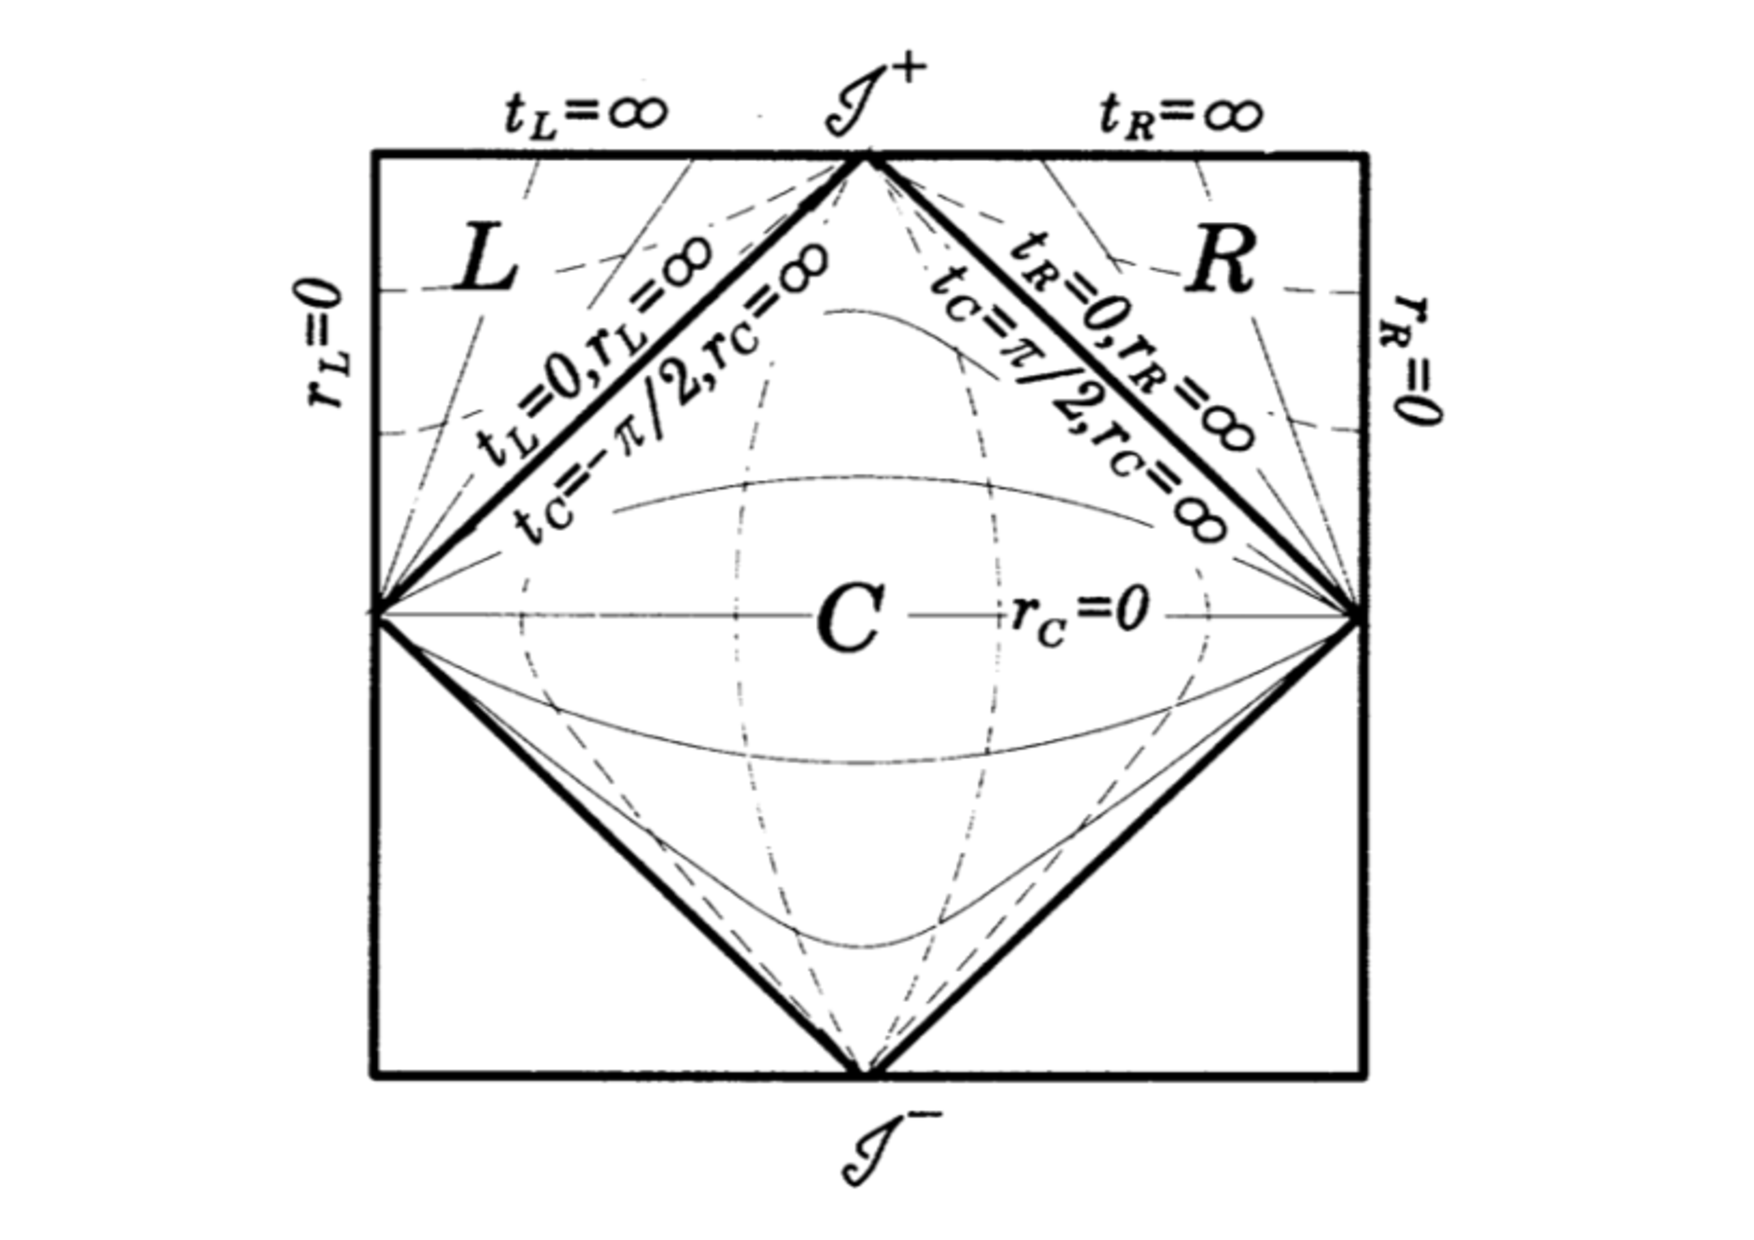
\includegraphics[width=8cm,angle=270]{desRL.pdf}
  \caption{Conformal Diagram of de Sitter space}
    \label{desRL}
  \end{center}
\end{figure}

\subsubsection{Open Chart}
\subsubsection{Scalar field on de Sitter Space}
次に,質量が$m$のfree scalar field $\varphi$について考える,lagrangianは次で与えられる,
\begin{align}
S=\int d^4x\biggr(\frac{1}{2}\sqrt{-g}(-g^{\mu\nu}\partial_{\mu}\varphi\partial_{\nu}\varphi-m^2\varphi^2-\xi R \varphi^2)\biggl)
\end{align}
ここで,今回は,作用の第三項に曲率とscalar fieldのカップリングを導入した.\footnote{\textcolor{red}{このように曲率との結合を考える正当性についてはもう少し学ぶ必要がありそう.}}また,その結合定数を$\xi$で与えた.この項は,理論上入る可能性があるが観測では曲率が0に近いので実際に必要であるかどうか難しいところである,今回は,$m_{eff}^2=m^2+\xi R$のように有効質量を用いることで普段と同様の扱いができることを利用して考える.ちなみに,de Sitter時空におけるRicci scalarは,
\begin{align}
  R=12H^{-2}
\end{align}
であるので,lagrangianは,
\begin{align}
  \label{1.60}
  \mathcal{L}&=\frac{1}{2}\sqrt{-g}(-g^{\mu\nu}\partial_{\mu}\varphi\partial_{\nu}\varphi-m^2\varphi^2-12H^{-2}\xi \varphi^2) \\
  \label{1.61}
  &=\frac{1}{2}\sqrt{-g}(-g^{\mu\nu}\partial_{\mu}\varphi\partial_{\nu}\varphi-m_{eff}^2\varphi^2)
\end{align}
とかける,ただし,有効質量は,
\begin{align}
  m_{eff}^2=m^2+12H^{-2}\xi
\end{align}
で定義した.このときの運動方程式は,EL方程式(\ref{EL})より,
\begin{align}
    \frac{1}{\sqrt{-g}}\partial_{\mu}\biggl(\sqrt{-g}g^{\mu\nu}\partial_{\nu}\varphi
\biggr)
    -m_{eff}^2\varphi=0
\end{align}
となる,ここで,Padmanの(4.108)式にあるように,
\begin{align}
  \label{1.65}
  \nabla_{\mu}\nabla^{\mu}\varphi=\frac{1}{\sqrt{-g}}\partial_{\mu}\biggl(\sqrt{-g}g^{\mu\nu}\partial_{\nu}\varphi\biggr)
\end{align}
であるので,運動方程式は,さらにシンプルな形にまとめられて,
\begin{align}
  \label{1.66}
  \biggl[g^{\mu\nu}\nabla_{\mu}\nabla_{\nu}-m_{eff}^2\biggr]\varphi=0
\end{align}
となる,この方程式は,flatな場合のKlein-Gordon方程式を重力がある時に拡張した形になっている.(偏微分$\partial$を共変微分$\nabla$に変えた形になっている.)
次に,$\varphi$をRとL領域においてモード展開する.場の演算子$\varphi$は,(\ref{1.66})式の解(固有関数モード)の線形結合で表されるので,
\begin{align}
  \varphi(t,r,\Omega)=\sum_{\Lambda}(\hat{\bm{a}}_{\Lambda}u_{\Lambda}(t,r,\Omega)+\hat{\bm{a}}^{\dagger}_{\Lambda}u^{*}_{\Lambda}(t,r,\Omega))
\end{align}
と展開できる.ただし,$u_{\Lambda}(t,r,\Omega)$は,(\ref{1.66})式を満たす固有関数である,
\begin{align}
  \label{1.68}
\biggl[g^{\mu\nu}\nabla_{\mu}\nabla_{\nu}-m_{eff}^2\biggr]u_{\Lambda}(t,r,\Omega)=0
\end{align}
この関数,すなわちopen chartのEuclidean vacuum におけるモード関数を求めるために,(\ref{1.68})式を$g^{\mu\nu}$が$g_{\mu\nu}$の逆行列であることに注意して,$(t,r,\Omega)$を用いて書き下すと,(具体的には,(\ref{1.65})式を用いて書き出すほうが楽である.ここで,$\sqrt{-g}=H^{-4}\sinh^3t\sinh^2r\sin\theta$であることを用いた.)
\begin{align}
  \biggl[\frac{1}{\sinh^3t}\frac{\partial}{\partial t}\sinh^3t\frac{\partial}{\partial t}-\frac{1}{\sinh^2t}\bm{L}^2_{H^3}+\frac{4}{9}-\nu^2\biggr]u(t,r,\Omega)=0
\end{align}
となる.この方程式はR,Lのそれぞれの領域で成り立つ.したがって,$(t,r)=(t_{R},r_{R}) or (t_{L},r_{L})$である,
また,ラプラシアン$L_{H^3}^2$と$\nu$はそれぞれ,
\begin{align}
  \bm{L}_{H^3}^2&=\frac{1}{\sinh^2r}\frac{\partial}{\partial r}\biggl(\sinh^2r\frac{\partial}{\partial r}\biggr)+\frac{1}{\sinh^2r}\bm{L}_{\Omega}^2 \\
  \bm{L}_{\Omega}^2&=\frac{1}{\sin\theta}\frac{\partial}{\partial \theta}\sin{\theta}\frac{\partial}{\partial \theta}+\frac{1}{\sin^2{\theta}}
  \frac{\partial^2}{\partial \phi^2} \\
  \nu&=\sqrt{\frac{9}{4}-\frac{m^2_{eff}}{H^{2}}}
\end{align}
で表される.Lagragianがローレンツ変換に対する対称性があるので,RとLは完全に対称な形で運動方程式が与えられる。まずモード関数$u_{\Lambda}(t,r,\Omega)$を$t$に関係する部分とそれ以外に分離する.
\begin{align}
  u_{\Lambda}(t,r,\Omega)&=\chi(t)Y_{plm}(r,\Omega)\\
  &=\chi(t)f_{pl}(r)Y_{lm}(\theta,\phi)
 \end{align}
 $\bm{L_{\Omega}^2}$部分は,固有値方程式,
\begin{align}
  L_{\Omega}^2Y_{lm}(\theta,\phi)=-l(l+1)Y_{lm}(\theta,\phi)
\end{align}
を満たし,固有値$l,m$によって特徴付けられる,(右辺の符号がマイナスであれば,この方程式は,ルジャンドルの陪微分方程式になる.)
また,$Y_{plm}(r,\Omega)$の部分は,\textcolor{red}{あとで確認するように,次の固有値方程式を満たすことがわかる.}
\begin{align}
  \bm{L}_{H^3}^2Y_{plm}(r,\Omega)&=-(1+p^2)Y_{plm}(r,\Omega) \\
  &or \\
 \bm{L}_{H^3}^2f_{pl}(r)Y_{lm}(\theta,\phi)&=-(1+p^2)f_{pl}(r)Y_{lm}(\theta,\phi)
\end{align}
そこでこれを,具体的に書き下すと
\begin{align}
\biggl(\frac{1}{\sinh^2r}\frac{\partial}{\partial r}\biggl(\sinh^2r\frac{\partial}{\partial r}\biggr)+\frac{1}{\sinh^2r}\bm{L}_{\Omega}^2\biggr)f_{pl}(r)Y_{lm}(\theta,\phi)=-(1+p^2)Y_{plm} \\
\label{1.80}
\therefore\biggl(\frac{1}{\sinh^2r}\frac{\partial}{\partial r}\biggl(\sinh^2r\frac{\partial}{\partial r}\biggr)-\frac{l(l+1)}{\sinh^2r}+(1+p^2)\biggr)f_{pl}(r)Y_{lm}(\theta,\phi)=0
\end{align}
ここで,$\xi=\cosh r$の座標変換をすれば,
\begin{align}
  \sinh r=\xi^2 -1, \hspace{4mm} \frac{\partial}{\partial r}=\frac{\partial \xi}{\partial r}\frac{\partial}{\partial \xi}=\sinh r\frac{\partial}{\partial \xi}
\end{align}
であるので,(\ref{1.80})式は,
\begin{align}
  \label{1.81}
\left(\left(\xi^2-1\right)\frac{\partial^2}{\partial \xi^2}+3 x \frac{\partial}{\partial \xi}-\frac{l (l+1)}{\xi^2-1}+(p^2+1)\right)f_{pl}(\xi)=0
\end{align}
のように書き換えられる.\footnote{ここまでの操作をまとめる.運動方程式は,4つの文字を含んだ偏微分方程式でむずかしいので,段階を分けて処理した.はじめに$\phi$について解き(固有値は$m$)次に,$\theta$についてといて(固有値は$l$)最後に,$r$について式を整理した.$r$だけの方程式になったのが,(\ref{1.80})式でありこれをとけば良い.}

この解は,\begin{align}
  f^l_p(\xi)=\frac{c_1 P_{i p-\frac{1}{2}}^{l+\frac{1}{2}}(\xi)+c_2 Q_{i p-\frac{1}{2}}^{l+\frac{1}{2}}(\xi)}{\sqrt[4]{\xi^2-1}}
\end{align}
となる.ここで,$P^{\mu}_{\nu}$は第1種ルジャンドルの陪関数であり,$Q^{\mu}_{\nu}$は第2種ルジャンドルの陪関数である.

ただし,$Q(\xi)$は$\xi=1$で正則でないので,$c_2=0$で落とせば,
\begin{align}
  f^l_p(\xi)=\frac{1}{\sqrt[4]{x^2-1}}c_1 P_{i p-\frac{1}{2}}^{l+\frac{1}{2}}(\xi)
\end{align}
最後に下座標系に戻すと.
\begin{align}
  \label{lugg}
  f^l_p(r)=\frac{1}{\sqrt{\sinh r}}c_1 P_{i p-\frac{1}{2}}^{l+\frac{1}{2}}(\cosh r)
\end{align}
となる.\footnote{\ref{ligg}式において,ルジャンドル多項式の上側のindexの符号は,全体にマイナスをかけても結果は変わらない.これは次のように理解できる.(\ref{1.81})式において,$l$を$l-1$に変えたもの微分方程式を考えると,
\begin{align}
\label{luggg}
\left(\left(\xi^2-1\right)\frac{\partial^2}{\partial \xi^2}+3 x \frac{\partial}{\partial \xi}-\frac{l (l-1)}{\xi^2-1}+(p^2+1)\right)f_{pl}(\xi)=0
\end{align}
その解は,$P^{l-\frac{1}{2}}$となる,さらに,$l\to-l$と変えると,微分方程式は,(\ref{luggg})式は,(\ref{1.81})式に一致する.したがって,
\begin{align}
  P^{-l-\frac{1}{2}}=P^{l+\frac{1}{2}}
\end{align}
であることがわかる.

また、\textcolor{red}{以下の関係も満たすことが確認できる}
\begin{equation}
  P^{\mu}_{\nu}=P^{\mu}_{-\mu-1}
\end{equation}
}
この解は,分母に$0$になる可能性がある因子があるが、積分をする際、波動関数全体に$\sinh r$がかかるので結果的に収束する項となる。


\begin{eqnarray}
\hat\phi(t,r,\Omega) = \sum_{\sigma,\ell,m} \int dp
\left[\,a_{\sigma p\ell m}\,u_{\sigma p\ell m}(t,r,\Omega)
+a_{\sigma p\ell m}^\dagger\,u^*_{\sigma p\ell m}(t,r,\Omega)\,\right]\,,
\label{phi}
\end{eqnarray}


\begin{eqnarray}
u_{\sigma p\ell m} = \frac{H}{\sinh t}\,
\chi_{p,\sigma}(t)\,Y_{p\ell m} (r, \Omega)\,.
\label{bdmf}
\end{eqnarray}

\begin{eqnarray}
\chi^{\sigma} = N_p^{-1} \sum_{q=R,L} \left[\,
 \alpha_q^\sigma\,P^q + \beta_q^\sigma\,P^{*\,q}
\,\right]\,,
\label{sty2}
\end{eqnarray}


\begin{eqnarray}
&&\alpha_R^\sigma = \frac{e^{\pi p} -i\sigma e^{-i\pi \nu}}{\Gamma (\nu+ip +\frac{1}{2})}\qquad,\qquad
\beta_R^\sigma =-\frac{e^{-\pi p} -i\sigma e^{-i\pi \nu}}{\Gamma (\nu-ip +\frac{1}{2})} \,\,,\\
&&\alpha_L^\sigma =\sigma\,\frac{e^{\pi p} -i\sigma e^{-i\pi \nu}}{\Gamma (\nu+ip +\frac{1}{2})}
\quad\,,\qquad
\beta_L^\sigma =-\sigma\,\frac{e^{-\pi p} -i\sigma e^{-i\pi \nu}}{\Gamma (\nu-ip +\frac{1}{2})}   \,\,.
\end{eqnarray}


\begin{eqnarray}
\chi^{*\,\sigma}=N_p^{-1}\sum_{q=R,L} \left[\,
{\beta^{*}{}_q}^{\!\!\!\sigma}\,P^q + {\alpha^{*}{}_q}^{\!\!\!\sigma}\,P^{*\,q}
\,\right]\,.
\end{eqnarray}

\begin{eqnarray}
\chi^I=N_p^{-1}\,M^I{}_J\,P^J\,,
\end{eqnarray}

\begin{eqnarray}
\chi^I=\left(\,\chi^\sigma\,,\chi^{*\,\sigma}\,\right)\,,\quad
M^I{}_J=\left(
\begin{array}{ll}
\alpha^\sigma_q & \beta^\sigma_q \vspace{3mm}\\
{\beta^{*}{}_q}^{\!\!\!\sigma} & {\alpha^{*}{}_q}^{\!\!\!\sigma} \\
\end{array}\right)\,,\quad
P^J=\left(\,P^R\,,P^L\,,P^{*\,R}\,, P^{*\,L}\,\right)\,.
\end{eqnarray}


\begin{eqnarray}
\phi(t)=a_I\,\chi^I=N_p^{-1}a_I\,M^I{}_J\,P^J\,,\qquad
a_I=\left(\,a_\sigma\,,\,a_\sigma^\dagger\,\right)\,,
\label{phi2}
\end{eqnarray}



\begin{eqnarray}
\phi(t)=N_p^{-1}b_J\,P^J\,,\qquad
b_J=\left(\,b_R\,,\,b_L\,,\,b_R^\dagger\,,\, b_L^\dagger\,\right)\,.
\label{phi3}
\end{eqnarray}


\begin{eqnarray}
a_J=b_I\left(M^{-1}\right)^I{}_J\,,\qquad
\left(M^{-1}\right)^I{}_J=\left(
\begin{array}{ll}
\xi_{q\sigma} & \delta_{q\sigma} \vspace{3mm}\\
\delta_{q\sigma}^* & \xi_{q\sigma}^* \\
\end{array}\right)\,,\qquad
\left\{
\begin{array}{l}
\xi=
\left(\alpha-\beta\,\alpha^{*\,-1}\beta^*\right)^{-1}\,,\vspace{3mm}\\
\delta=-\alpha^{-1}\beta\,\xi^*\,.
\end{array}
\right.
\label{xidelta1}
\end{eqnarray}


\begin{eqnarray}
a_\sigma=\sum_{q=R,L}\left[\,\xi_{q\sigma}\,b_q+\delta_{q\sigma}^*\,b_q^\dagger\,\right]\,.
\label{ab}
\end{eqnarray}


\begin{eqnarray}
|{\rm BD}\rangle = \exp\left(\frac{1}{2}\sum_{i,j=R,L}m_{ij}\,b_i^\dagger\, b_j^\dagger\right) |R\rangle|L\rangle\,,
\label{bogoliubov1}
\end{eqnarray}

\begin{eqnarray}
m_{ij}=-\delta_{i\sigma}^*\left(\xi^{-1}\right)_{\sigma j}
=-\frac{\Gamma\left(\nu-ip+1/2\right)}{\Gamma\left(\nu+ip+1/2\right)}
\frac{2\,e^{i\pi\nu}}{e^{2\pi p}+e^{2i\pi\nu}}
\left(
\begin{array}{cc}
\cos \pi\nu & i\sinh p\pi \vspace{1mm}\\
i\sinh p\pi & \cos \pi\nu \\
\end{array}
\right)\,.
\label{mij1}
\end{eqnarray}


\begin{eqnarray}
m_{ij}=e^{i\theta}\frac{\sqrt{2}\,e^{-p\pi}}{\sqrt{\cosh 2\pi p+\cos 2\pi\nu}}
\left(
\begin{array}{cc}
\cos \pi\nu & i\sinh p\pi \vspace{1mm}\\
i\sinh p\pi & \cos \pi\nu \\
\end{array}
\right)\,,
\label{mij2}
\end{eqnarray}



\begin{eqnarray}
c_R = u\,b_R + v\,b_R^\dagger \,,\qquad\quad
c_L = \bar{u}\,b_L + \bar{v}\,b_L^\dagger\,,
\label{bc}
\end{eqnarray}


\begin{eqnarray}
|{\rm BD}\rangle = \exp\left(\gamma_p\,c_R^\dagger\,c_L^\dagger\,\right)|R'\rangle|L'\rangle\,,
\label{bogoliubov2}
\end{eqnarray}


\begin{eqnarray}
c_R\,|{\rm BD}\rangle= \gamma_p\,c_L^\dagger\,|{\rm BD}\rangle \,,\qquad
c_L\,|{\rm BD}\rangle = \gamma_p\,c_R^\dagger\,|{\rm BD}\rangle\,.
\label{consistency}
\end{eqnarray}

\begin{eqnarray}
&&\omega\,u + v -\gamma_p\,\zeta\,\bar{v}^* =0 \ , \qquad
\zeta\,u - \gamma_p\,\bar{u}^* - \gamma_p\,\omega\,\bar{v}^* =0\,,
\label{system1}\\
&&\omega\,\bar{u} + \bar{v} -\gamma_p\,\zeta\,v^* =0 \ , \qquad
\zeta\,\bar{u} - \gamma_p\,u^* - \gamma_p\,\omega\,v^* =0\,.
\label{system2}
\end{eqnarray}


\begin{eqnarray}
\gamma_p=\frac{1}{2\zeta}\left[-\omega^2+\zeta^2+1-\sqrt{\left(\omega^2-\zeta^2-1\right)^2-4\zeta^2}\,\right]\,,
\label{gammap}
\end{eqnarray}


\begin{eqnarray}
\gamma_p = i\frac{\sqrt{2}}{\sqrt{\cosh 2\pi p + \cos 2\pi \nu}
 + \sqrt{\cosh 2\pi p + \cos 2\pi \nu +2 }}\,.
\label{gammap2}
\end{eqnarray}


\begin{eqnarray}
\rho_L ={\rm Tr}_{R}\,|{\rm BD}\rangle\langle{\rm BD}|
=\left(1-|\gamma_p|^2\,\right)\sum_{n=0}^\infty |\gamma_p |^{2n}\,|n;p\ell m\rangle\langle n;p\ell m|\,,
\label{densitymatrix1}
\end{eqnarray}

\begin{eqnarray}
\sum_{n=0}^\infty |\gamma_p |^{2n}=\lim_{n\rightarrow\infty}\frac{1-|\gamma_p|^{2n}}{1-|\gamma_p|^2}\xrightarrow{|\gamma_p|<1}\frac{1}{1-|\gamma_p|^2}\,.
\end{eqnarray}


\begin{eqnarray}
S(p,\nu)=-{\rm Tr}\,\rho_L(p)\,{\rm log}\,\rho_L(p)
=-{\rm log}\,\left(1-|\gamma_p|^2\right)
-\frac{|\gamma_p|^2}{1-|\gamma_p|^2}\,{\rm log}\,|\gamma_p|^2\,.
\label{s}
\end{eqnarray}
Note that this formula is derived under the condition $|\gamma_p|<1$.

cap3

cap4
\chapter{量子操作}

%
%
\appendix
%
\chapter{特殊関数}
\section{ルジャンドル関数}
\subsection{ルジャンドルの微分方程式}
\section{球面調和関数}
\section{球面調和関数 in hyperbolic}

必要に応じて
\subsection{様々な計算手法と近似法}
\subsubsection{鞍点法}
\chapter{Entanglement Entropy in Rindler Space}


\chapter{相対論と場の理論からの準備}
\section{一般相対論からの準備}
はじめに,時空を記述するために必要な道具として,数学的な表現を考える.まず時空は集合として扱え,また,点の集積点などを含む位相空間,(距離を定義したい)これに座標を張るために多様体を用意する.多様体から曲率を定義したい.距離の測り方としてメトリックを導入する.
\subsubsection{ブラックホール(BH)}
事象の水平線で囲まれた内側が存在し,その内側の部分をBHと呼ぶ.
\subsection{相対論的運動学}
以下の議論では,ミンコフスキー(Minkowski)計量$\eta_{\mu\nu}$の符号を
\begin{eqnarray}
\label{D1}
\eta_{\mu\nu}=
\left(\begin{array}{cccc}-1 & 0 & 0 & 0 \\
0 & 1 & 0 & 0 \\
0 & 0 & 1 & 0 \\
0 & 0 & 0 & 1
\end{array}\right)
\end{eqnarray}
に定める.
このとき,時空間隔は,
\begin{eqnarray}
ds^2=\eta_{\mu\nu}dx^{\mu}dx^{\nu}
\end{eqnarray}
で与えられる.粒子とともに動く観測者によってによって測られる$\tau$を固有時と呼び,この系における粒子の微小時間間隔は,
\begin{eqnarray}
\label{tau}
\eta_{\mu\nu}dx^{\mu}dx^{\nu}=-d\tau^2
\end{eqnarray}
で与えられる.

質量が0でない粒子を考えてときの,単位固有時あたりの粒子の座標変化は,4元速度と呼ばれ,
\begin{eqnarray}
u^{\mu}=\frac{dx^{\mu}}{d\tau}
\end{eqnarray}
で定義される.この四元ベクトルは,(\ref{tau})式によって規格化されていて,
\begin{eqnarray}
\label{4v}
\eta_{\mu\nu}u^{\nu}u^{\mu}=-1
\end{eqnarray}
を満たす.以上から,四元速度$u^{\mu}$は,
\begin{eqnarray}
\label{4vv}
(u^{\mu})=\biggl(\frac{c}{\sqrt{1-v^2}},\frac{\bm{v}}{{\sqrt{1-v^2}}}\biggr)
\end{eqnarray}
ここで,$|\bm{v}|=v$である.また,粒子の静止質量を$m$とすれば,粒子の四元運動量が
\begin{eqnarray}
P^{\mu}=mu^{\mu}
\end{eqnarray}
が定義できる.(\ref{4vv})式から,
\begin{eqnarray}
(P^{\mu})&=&\biggl(\frac{mc}{\sqrt{1-v^2}},\frac{m\bm{v}}{{\sqrt{1-v^2}}}\biggr)  \vspace{4mm} \\
&=&\biggl(\dfrac{E}{c},\bm{P}\biggr)
\end{eqnarray}
である.これより,粒子の静止系からみた速度$\bm{v}$と四元運動量の関係は,
\begin{eqnarray}
\label{vp}
\bm{v}=c\frac{\bm{P}}{P^{0}}=c^2\frac{\bm{P}}{E}
\end{eqnarray}
となることに注意したい.
\begin{empheqboxed}
\

四元速度の規格化条件(\ref{4v})式より,四元運動量$P^{\mu}$は,
\begin{eqnarray}
\label{OS}
\eta_{\mu\nu}P^{\mu}P^{\mu}+m^2=0
\end{eqnarray}
のOn-shell条件が課される.
\end{empheqboxed}

粒子の持つエネルギーは,この四元運動量を用いて二通りで表されて,
\begin{eqnarray}
E=cP^{0}&=&\dfrac{mc^2}{\sqrt{1-\beta^2}} \\
&=&\sqrt{c^2P^2+m^2c^4}
\end{eqnarray}
となる.ただし,$|\bm{P}|=P$である.
\subsection{計量に関する有用な公式}
対角化可能な行列$M$に対して,$\mathrm{Tr}\ln M$を考える.対数$\ln$のテイラー展開は,
\begin{eqnarray}
\log(x+1)=x-\frac{1}{2}x^2+\frac{1}{3}x^3+\cdots
\end{eqnarray}
あるいは,
\begin{eqnarray}
\log(x)=(x-1)-\frac{1}{2}(x-1)^2+\frac{1}{3}(x-1)^3+\cdots
\end{eqnarray}
と展開できるので,$\mathrm{Tr}\ln M$も同様に計算できて,
\begin{eqnarray}
\mathrm{Tr}\ln M&=&\mathrm{Tr}\biggl((M-E)-\frac{1}{2}(M-E)^2+\cdots\biggr) \nonumber \\
&=&\mathrm{Tr}\biggl(A(N-E)A^{-1}-\frac{1}{2}A(N-E)^2A^{-1}+\cdots\biggr) \nonumber \\
&=&\mathrm{Tr}\biggl(A(\ln N)A^{-1}\biggr) \nonumber \\
&=&\mathrm{Tr}\ln N \nonumber \\
&=&\log\lambda_1+\ln\lambda_2+\cdots+\ln\lambda_n \nonumber \\
&=&\ln\lambda_1\lambda_2\cdots\lambda_n \nonumber \\
&=&\ln\det M
\end{eqnarray}
ここで,$N$は$M$を対角化行列$A$で対角化したものであり,3行目から4行目の変形は,トレースの性質を用いた.
\begin{empheqboxed}
\

したがって,対角化可能な行列$M$に対して,
\begin{eqnarray}
\label{trdet}
\mathrm{Tr} \ln M=\ln \det M
\end{eqnarray}が成立する.
\end{empheqboxed}
\footnote{
(\ref{trdet})式は,
\begin{eqnarray}
\label{iii}
\det M=\exp(\mathrm{Tr}\ln M)
\end{eqnarray}
と書き換えられて,さらに,
\begin{eqnarray}
M=\exp G
\end{eqnarray}
と定めることで,(\ref{iii})式の右辺が$G$で表されて,
\begin{eqnarray}
\label{iiii}
\det M=\exp(\mathrm Tr G)
\end{eqnarray}を得る.この式は,郡$M$と代数$G$(generator)の間の関係と見ることもできる.いま,$\det M=1$を満たすような変換行列(回転)を考えると,(\ref{iiii})式から$\exp(\mathrm{Tr} G)=1$すなわち,$\mathrm{Tr} G=0$となる.$G$の例としてパウリ演算子などがあげられる.同様に,$\det M>1$(拡大)なる変換に対するgeneratorは,$\mathrm{Tr} G>0$であり,$\det M>1$(縮小)なる変換に対するgeneratorは,$\mathrm{Tr} G<0$となることがわかる.}

微分とトレースは可換であるから,(\ref{trdet})式の両辺を変分すると,
\begin{eqnarray}
{\delta \det M\over \det M}=Tr M^{-1}\delta M
\end{eqnarray}
なる関係が得られる.これを計量に適応すれば,
\begin{empheqboxed}
\begin{eqnarray}
\label{ggg}
\delta g=g g^{\mu\nu}\delta g_{\mu\nu}
\end{eqnarray}
\end{empheqboxed}
なる有用な公式が得られる.今度は行列式ではなく,$g_{\mu\nu}$の変分を求める.初めに,$\delta(g_{\mu\nu}g^{\mu\lambda})=0$であるのから,
\begin{eqnarray}
g_{\mu\nu}\delta g^{\mu\lambda}=-g^{\mu\lambda}\delta g_{\mu\nu}
\end{eqnarray}
であるが,$g^{\delta \nu}$を両辺にかけて足をつぶせば,
\begin{empheqboxed}
\begin{eqnarray}
\label{gggg}
\delta g^{\lambda\delta }=-g^{\mu\lambda}g^{\nu\delta}\delta g_{\mu\nu}
\end{eqnarray}
\end{empheqboxed}
なる関係が得られる.すなわち,$\delta g^{\lambda\delta }$の添え字は,計量$g_{\mu\nu}$でしていけないことがわかる.さらに,(\ref{ggg})式と,(\ref{gggg})式を用いいれば,
\begin{eqnarray}
\label{hen-g}
\delta\sqrt{-g}&=&\frac{1}{2}\sqrt{-g}g^{\mu\nu}\delta g_{\mu\nu} \\
&=&-\frac{1}{2}\sqrt{-g}g_{\mu\nu}\delta g^{\mu\nu}
\end{eqnarray}
などが計算できる.
\subsection{共変微分}
共変微分は,座標によらない微分概念である.ベクトル場を考えて,ある曲線に沿って点$P$の接空間で定義されるベクトルを点$Q$へ並行移動する.並行移動した点$P$で定義されていたベクトルを点$Q$で定義されている元のベクトルとの差を考えるのが共変微分である.ここで,並行移動とは,点$P$で定義されている接空間の基底ベクトルを他の点$Q$で定義されている接空間の基底ベクトルで表すことである.
\begin{empheqboxed}
\

例えば,一階共変反変テンソル$A^{\mu}_{\ \nu}$の共変微分は,
\begin{eqnarray}
\nabla_{\rho}A^{\mu}_{\ \ \nu}=\partial_{\rho}A^{\mu}_{\ \ \nu}+\Gamma^{\mu}_{\rho\lambda}A^{\lambda}_{\ \ \nu}-\Gamma^{\lambda}_{\rho\nu}A^{\mu}_{\ \ \lambda}
\end{eqnarray}
となる.(ベクトルの上付き添え字でクリストフェルと縮約を取るときは,符号が正であると覚えておけば良い,)
ここで,クリストフェル(Christoffel)$\Gamma^{\mu}_{\nu\lambda}$は,以下で表される.
\begin{eqnarray}
\label{Ch}
\Gamma^{\mu}_{\nu\lambda}=\frac{1}{2}g^{\mu\rho}(\partial_\nu g_{\lambda\rho}+\partial_\lambda g_{\nu\rho} - \partial_\rho g_{\nu\lambda})
\end{eqnarray}

\end{empheqboxed}
ただし,totion freeを課した.ここで,クリストフェル$\Gamma^{\mu}_{\nu\lambda}$は,テンソルでなく座標変換に対して,
\begin{eqnarray}
\Gamma^{\prime \alpha}_{\ \beta\gamma}=\frac{\partial x^{\prime\alpha}}{\partial x^{\mu}}\frac{\partial x^{\nu}}{\partial x^{\prime\beta}}\frac{\partial x^{\lambda}}{\partial x^{\prime\gamma}}\Gamma^{\mu}_{\ \nu\lambda}+\frac{\partial^2 x^{\rho}}{\partial x^{\prime \beta}\partial x^{\prime \gamma}}\frac{\partial x^{\prime \alpha}}{\partial x^{\rho}}
\end{eqnarray}
あるいは,
\begin{eqnarray}
\Gamma^{\prime \alpha}_{\ \beta\gamma}=\frac{\partial x^{\prime\alpha}}{\partial x^{\mu}}\frac{\partial x^{\nu}}{\partial x^{\prime\beta}}\frac{\partial x^{\lambda}}{\partial x^{\prime\gamma}}\Gamma^{\mu}_{\ \nu\lambda}-\frac{\partial x^{\nu}}{\partial x^{\prime\beta}}\frac{\partial x^{\lambda}}{\partial x^{\prime\gamma}}\frac{\partial^2 x^{\prime \alpha}}{\partial x^{\nu}\partial x^{\lambda}}
\end{eqnarray}
と変換する.

(\ref{Ch})式で,クリストフェルの縮約をとると,
\begin{eqnarray}
\label{Chdetg}
\Gamma^{\mu}_{\nu\mu}=\frac{1}{2}g^{\mu\rho}\partial_\nu g_{\mu\rho}=\frac{\partial_{\nu} g}{2g}=\frac{\partial_{\nu} \sqrt{-g}}{\sqrt{-g}}
\end{eqnarray}
二番目の等号は,(\ref{ggg})式を用いた.
これより,ベクトルの発散に関する有用な公式,
\begin{eqnarray}
\label{di32}
\nabla_{\mu}A^{\mu}&=&\partial_{\mu}A^{\mu}+\Gamma^{\mu}_{\mu\nu}A^{\nu} \nonumber \\
&=&\partial_{\mu}A^{\mu}+\frac{\partial_{\mu} \sqrt{-g}}{\sqrt{-g}}A^{\mu} \nonumber \\
&=&\frac{1}{\sqrt{-g}}\partial_{\mu}(\sqrt{-g}A^{\mu})
\end{eqnarray}
が導かれる.また,ベクトル$A^{\mu}$がスカラー$\phi$の$\grad$から求まるとき,$A^{\mu}=\nabla^{\mu} \phi=g^{\mu\nu}\partial_{\nu}\phi$となるので,
これを(\ref{di32})式に代入すると,
\begin{eqnarray}
\nabla_{\mu}\nabla^{\mu}\phi=\frac{1}{\sqrt{-g}}\partial_{\mu}(\sqrt{-g}g^{\mu\nu}\partial_{\nu}\phi)
\end{eqnarray}
さらに,高階テンソルついても,$A^{\mu\nu\cdots}$が,添え字に関して反対称であれば全く同様な式が得られる.以上をまとめれば,
\begin{empheqboxed}
\begin{eqnarray}
\label{a34}
\nabla_{\mu}A^{\mu}=\frac{1}{\sqrt{-g}}\partial_{\mu}(\sqrt{-g}A^{\mu})
\end{eqnarray}
\begin{eqnarray}
\nabla_{\mu}\nabla^{\mu}\phi=\frac{1}{\sqrt{-g}}\partial_{\mu}(\sqrt{-g}g^{\mu\nu}\partial_{\nu}\phi)
\end{eqnarray}
\end{empheqboxed}
となる.

ただし,ここまでの計算では,計量条件(メトリシティー),
\begin{eqnarray}
g^{\mu\nu}_{\ \ ;\mu}=0
\end{eqnarray}
あるいは,この式から求まる関係,
\begin{eqnarray}
\label{metometo}
g_{\mu\nu,\lambda}=g_{\mu\rho}\Gamma^{\rho}_{\nu\lambda}+g_{\nu\rho}\Gamma^{\rho}_{\mu\lambda}
\end{eqnarray}
を仮定して計算した.
\subsection{測地線方程式}
アフィンパラメーター$\lambda$とすると,運動量$P^{\mu}$は粒子の位置座標$x^{\mu}$を用いて,
\begin{eqnarray}
\label{D2}
P^{\mu}={d x^{\mu}\over d\lambda}
\end{eqnarray}で定められる,ここで,アフィンパラメーターとは,(\ref{tau})式で定義された固有時のアフィン変換
\begin{eqnarray}
\lambda=a\tau+b
\end{eqnarray}で表されるようなパラメータである.
粒子が重力の影響を受けながら運動するとき,重力以外が働かなければその粒子の軌道は,
\begin{eqnarray}
\label{Go}
{d P^{\mu}\over d\lambda}+\Gamma^{\mu}_{\nu\sigma}P^{\nu}P^{\sigma}=0
\end{eqnarray}
にしたがう.
\subsection{曲率}
リーマン(Riemann Tensor)テンソルについて簡単に確認する.計量$g_{\mu\nu}$に二回微分に相当する幾何学量であり,重力の有無を判断する良い指標になる.リーマンテンソルは,共変微分の交換関係に現れて,
\begin{eqnarray}
\label{RRR}
\nabla_{\lambda}\nabla_{\delta}A^{\mu}-\nabla_{\delta}\nabla_{\lambda}A^{\mu}=\bigl[\nabla_{\lambda},\nabla_{\delta}\bigr]=R^{\mu}_{\nu\lambda\delta}A^{\nu}
\end{eqnarray}
と表せる.
\begin{empheqboxed}
\

$R^{\mu}_{\nu\lambda\delta}$をあらわに書き表せば,
\begin{eqnarray}
\label{rie}
R^{\mu}_{\nu\lambda\delta}=\partial_{\lambda}\Gamma^{\mu}_{\nu\delta}-\partial_{\delta}\Gamma^{\mu}_{\nu\lambda}+\Gamma^{\mu}_{\rho\lambda}\Gamma^{\rho}_{\nu\delta}-\Gamma^{\mu}_{\rho\delta}\Gamma^{\rho}_{\nu\lambda}
\end{eqnarray}
で定義される.さらに,リーマンテンソルの縮約をとったリッチテンソル(Ricci tensor)は,
\begin{eqnarray}
\label{rct}
R_{\mu\nu}=R^{\lambda}_{\mu\lambda\nu}
\end{eqnarray}
であり,さらに縮約をとったリッチスカラーは,
\begin{eqnarray}
\label{rcs}
R=g^{\mu\nu}R_{\mu\nu}
\end{eqnarray}
で定義される.リーマンテンソルには,添字の循環に対して対称で,
\begin{eqnarray}
\label{Rcycle}
R^{\lambda}_{\mu\nu\sigma}+R^{\lambda}_{\nu\sigma\mu}+R^{\lambda}_{\sigma\mu\nu}=0
\end{eqnarray}を満たす.
\end{empheqboxed}
あとで,必要になるので,(\ref{rie}),(\ref{rct}),(\ref{rcs})式で定義される曲率の変分を求めておく.まずは,計量を共変微分したものの変分を求めることから始めていく,
\begin{eqnarray}
\label{hendg}
\nabla_{\lambda}(\delta g_{\mu\nu})=\delta g_{\mu\nu,\lambda}-\Gamma_{\mu\lambda}^{\tau}\delta g_{\tau\nu}-\Gamma_{\nu\lambda}^{\tau}\delta g_{\tau\mu}
\end{eqnarray}
となる,この式からも分るように,偏微分と変分は交換するが,共変微分と変分は交換しない,次にクリストフェルの変分を考える.(\ref{Ch})式より,
\begin{eqnarray}
\delta \Gamma^{\mu}_{\nu\lambda}=\frac{1}{2}\delta\biggl(g^{\mu\rho}(\partial_\nu g_{\lambda\rho}+\partial_\lambda g_{\nu\rho} - \partial_\rho g_{\nu\lambda})\biggr)
\end{eqnarray}
を(\ref{hendg})式を用いて計算すると,
\begin{eqnarray}
\delta \Gamma^{\mu}_{\nu\lambda}=\frac{1}{2}g^{\mu\rho}(\delta g_{\lambda\rho;\nu}+\delta g_{\nu\rho;\lambda} -\delta g_{\nu\lambda;\rho})
\end{eqnarray}
を得る.着目すべき点は,テンソルでないクリストフェルの変分は,テンソルとして振る舞うことである.同様に,このクリストフェルの変分に対する共変微分を考える.共変微分の定義から頑張って計算すると,
\begin{eqnarray}
\label{dhench}
\nabla_{\alpha}(\delta \Gamma^{\mu}_{\nu\lambda})=\delta \Gamma^{\mu}_{\nu\lambda;\alpha}=\frac{1}{2}g^{\mu\rho}(\delta g_{\lambda\rho;\nu\alpha}+\delta g_{\nu\rho;\lambda\alpha} -\delta g_{\nu\lambda;\rho\alpha})
\end{eqnarray}
を得る,これらを用いれば,リーマンテンソルの変分が計算できる.(\ref{rie})式から,
\begin{eqnarray}
\label{henri}
\delta R^{\mu}_{\nu\lambda\delta}&=&\delta\biggl(\partial_{\lambda}\Gamma^{\mu}_{\nu\delta}-\partial_{\delta}\Gamma^{\mu}_{\nu\lambda}+\Gamma^{\mu}_{\rho\lambda}\Gamma^{\rho}_{\nu\delta}-\Gamma^{\mu}_{\rho\delta}\Gamma^{\rho}_{\nu\lambda}
\biggr)\nonumber \\
&=&\delta\Gamma^{\mu}_{\nu\delta;\lambda}-\delta\Gamma^{\mu}_{\nu\lambda;\delta}
\end{eqnarray}
となるが,(\ref{dhench})式から計量を用いて表すこともできる,(\ref{henri})式で,縮約をとると,リッチテンソルを変分した値が得られて,
\begin{eqnarray}
\label{henrct}
\delta R_{\mu\nu}&=&\delta R^{\lambda}_{\mu\lambda\nu}=\delta\Gamma^{\lambda}_{\mu\nu;\lambda}-\delta\Gamma^{\lambda}_{\mu\lambda;\nu}\nonumber \\
&=&\frac{1}{2}\biggl(\delta g_{\lambda\mu;\nu}^{\quad \ \  ;\lambda}+\delta g_{\lambda\nu;\mu}^{\quad \ \  ;\lambda}-g^{\tau\lambda}\delta g_{\lambda\tau;\mu\nu}-\delta g_{\mu\nu;\lambda}^{\quad \ \  ;\lambda}\biggr)
\end{eqnarray}
となる.最後に,リッチスカラーについて変分をとる.(\ref{rcs})式より,
\begin{eqnarray}
\delta R=\delta(g^{\mu\nu}R_{\mu\nu})=g^{\mu\nu}\delta R_{\mu\nu}+R_{\mu\nu}\delta g^{\mu\nu}
\end{eqnarray}
となり,(\ref{henrct})式と,添字の対称性に注意して計算すると,
\begin{eqnarray}
\delta R=\delta g_{\mu\nu}^{\quad ;\mu\nu}-g^{\mu\nu}\delta g_{\mu\nu;\lambda}^{\quad \ \ ;\lambda}+R_{\mu\nu}\delta g^{\mu\nu}
\end{eqnarray}
が得られる.この式は,重力場の作用からアインシュタイン方程式を導く際に有用である.
\subsection{不変体積要素}
時空の計量$g_{\mu\nu}$の行列式を$g=\det(g_{\mu\nu})$で定義する.このとき,時空の不変体積要素は,$\sqrt{-g}d^4x$となる.四元運動量も四元ベクトルであるので不変体積要素も同様に$\sqrt{-g}d^4P$となる.そこで,8次元位相空間における不変体積要素は,$-gd^4xd^4P$である.実際の粒子の運動を考えるときは,8次元でなく,
\begin{eqnarray}
\label{Os}
P_{\mu}P^{\mu}+m^2=0
\end{eqnarray}
(\ref{OS})式で表されるOn-shell条件を満たすように運動する.したがって,位相空間の分配関数$f(x,P)$は,8次元に埋め込まれた7次元超曲面上に値を持つ.さらに,粒子の持っているエネルギー$E$は正であるはずなので,$E=P^{0}\geqslant0$の条件が課される.(これ以降,Os-shell条件を満たすような粒子のエネルギー$P^0$は,$E$と書くことにする.)

運動量にはこのような二つの制約が課されるので,次のような三次元運動量要素$d\Pi$を定義することは有用である.
\begin{eqnarray}
\label{D3}
d\Pi=\frac{\sqrt{-g}d^4P}{(2\pi)^3}\Theta(P^{0})\delta_{D}(P_{\mu}P^{\mu}+m^2)
\end{eqnarray}
ここで,$\Theta(P^{0})$は,階段関数(step function)でこの値は,本義ローレンツ変換の元で不変に保たれる.
よって,(\ref{D3})式の右辺もまた一般座標変換に対して不変なスカラーである.%\footnote{\textcolor{red}{ローレンツ不変だから一般座標変換不変にある????????}}
このような積分要素を定義すれば,上の要請を満たすような物理的な粒子について考えることになるので,$P^{0}$について先に積分してしまう.\footnote{積分要素であり,あとで積分することになるので先に行っておく}
(\ref{D3})式に現れるデルタ関数は,$f(x)=0$の解を$x_p$とするとき
\begin{empheqboxed}
\begin{eqnarray}
\label{D4}
\delta_{D}(f(x))=\sum_{p}{\delta_{D}(x-x_p) \over |f^{\prime}(x_p)|}
\end{eqnarray}
\end{empheqboxed}
なる性質がある.今,デルタ関数の中身のOn-shell条件(\ref{Os})式は,
$P^{0}=E$についてとくと(時空の構造によって,内積の値がかわることに注意する.)
\begin{eqnarray}
g_{00}(P^0)^2+2g_{0i}P^0P^i+g_{ij}P^iP^j+m^2=0
\end{eqnarray}から,
\begin{eqnarray}
E={g_{0i}P^i+\sqrt{(g_{0i}P^i)^2-g_{00}(g_{ij}P^iP^j+m^2)}\over -g_{00}}
\end{eqnarray}
となる,(\ref{D4})式との対応は,$|f^{\prime}(x_p)|$が$2g_{00}P^0+2g_{0i}P^i=2\sqrt{(g_{0i}P^i)^2-g_{00}(g_{ij}P^iP^j+m^2)}$であるので,具体的に,(\ref{D3})式の$P^0$に関する積分を実行すると,
\begin{eqnarray}
d\Pi=\dfrac{\sqrt{-g}d^3P}{2\sqrt{(g_{0i}P^i)^2-g_{00}(g_{ij}P^iP^j+m^2)}}
\end{eqnarray}
が得られる.
\begin{empheqboxed}
\

ミンコフスキー時空(\ref{D1})で不変体積要素は
\begin{eqnarray}
\label{D8}
d\Pi={\sqrt{-g}d^3P\over (2\pi)^32E}
\end{eqnarray}
となる.
\end{empheqboxed}
\subsection{四元流束(particle 4-flow)}
四元流束を後で使うので,ここで定義しておく,局所ミンコフスキー時空では\footnote{$\sqrt{-g}=1$となるので,普通に積分すればよいことになる.}(\ref{C3})式で定義した粒子の数密度が,(\ref{D8})式を用いて書き直せて,
\begin{eqnarray}
n(\bm{x},t)=2\int d\Pi P^0f(x,P) .
\end{eqnarray}
この値は四元運動量を用いて四元ベクトルに拡張子できて,
\begin{eqnarray}
\label{D13}
N^{\mu}(\bm{x},t)=2\int d\Pi P^{\mu}f(x,P)
\end{eqnarray}
が定義できる.これは,ミンコフスキー時空で四元流束とよばれる.四元ベクトルの成分で,書けば見慣れた形にになる.
\begin{eqnarray}
(N^{\mu})=(n,\bm{j})
\end{eqnarray}

\section{古典場の理論}
この節では,簡単に古典場の理論をまとめておく.本論文ではスカラー場のみを扱うので,簡単のために以下では,実スカラー場$\phi$について見ていくことにする.
\begin{empheqboxed}
\

古典的な場を考えると,この場$\phi$は作用原理から運動方程式,
\begin{eqnarray}
\label{eleq}
\dfrac{\delta S}{\delta \phi}=0
\end{eqnarray}
を満たす.具体的にラグラジアン密度を用いて表すと,
\begin{eqnarray}
\label{EL}
\frac{\partial \sqrt{-g}\mathcal{L}}{\partial \phi}-
\partial_{\mu}\frac{\partial \sqrt{-g}\mathcal{L}}{\partial(\partial_{\mu} \phi)}=0
\end{eqnarray}
のオイラーラグランジュ(Euler-Lagrange)方程式にしたがうことがわかる.
\end{empheqboxed}
これを出発点として,ラグラジアンとエネルギー運動量テンソルの関係を一般の時空で議論しよう.


\subsection{ネーターカレント(Noether current)}
保存則と対称性の関係は,ネーター(Noether)の定理によって表される.
考えている系の物理をラグラジアン密度を用いて表すことができるとするときについて考える.この系を支配する物理法則,あるいは運動方程式がある変換について不変であるとき,その系には必ず保存則が存在する.ここで,ある変換で運動方程式が不変であるということは,\textbf{作用が不変,あるいは作用の変化が表面項だけ}で与えられる場合である.
いま,簡単のために,
\begin{eqnarray}
\label{xn}
&x^{\mu}\rightarrow \overline{x}^{\mu}={x}^{\mu}+\overline{\delta}x^{\mu}& \\
\label{pn}
&\phi\rightarrow\overline{\phi}(\overline{x})=\phi(x)+\overline{\delta}\phi(x)&
\end{eqnarray}
のように,$\phi$と$x$を同時に変換する場合を考える.ここで注意すべきことは,$\phi$の変換が同じ座標値で行う変分でないことである.すなわち,
\begin{eqnarray}
\label{a64aa}
\overline{\delta}\phi(x)&=&\overline{\phi}(\overline{x})-\phi(x) \nonumber \\
&=&\overline\phi(x+\delta x)-\phi(x) \nonumber \\
&=&\delta\phi(x)+\phi_{,\mu}\overline{\delta}x^{\mu}
\end{eqnarray}
となっている.(\ref{a64aa})式の結果を見ると,変分$\overline{\delta}\phi(x)$には,きちんと$\phi(x)$の変分と$x$の変分からくる項が含まれている.$x$に関する変分を考えず,$\phi(x)$だけの変分を考えると時は$\delta x=0$となるので,確かに$\overline{\delta}\phi(x)=\delta\phi(x)$となっている.

同様に,$\sqrt{-g}\mathcal{L}$の(\ref{pn})式による変化量と変分の間の関係は,$\sqrt{-g}\mathcal{L}$全体を$x$の関数として捉えれば,
\begin{eqnarray}
\label{a24}
\overline{\delta}(\sqrt{-g}\mathcal{L})&=&\sqrt{-g(\overline{x})}\mathcal{L}(\overline{x})-\sqrt{-g(x)}\mathcal{L(x)} \nonumber \\
&=&\delta(\sqrt{-g}\mathcal{L})+\partial_{\mu}(\sqrt{-g}\mathcal{L})\overline{\delta}x^{\mu}
\end{eqnarray}
である.(\ref{a24})式の右辺第1項は,
\begin{eqnarray}
\label{a25}
\delta(\sqrt{-g}\mathcal{L})&=&\frac{\partial \sqrt{-g}\mathcal{L}}{\partial \phi}\delta \phi+\frac{\partial \sqrt{-g}\mathcal{L}}{\partial(\partial_{\mu} \phi)}\delta \partial_{\mu}\phi \nonumber \\
&=&\partial_{\mu}\biggl(\frac{\partial \sqrt{-g}\mathcal{L}}{\partial(\partial_{\mu} \phi)}\delta\phi\biggr)
\end{eqnarray}
と書き直せる.一行目から二行目の変形は,運動方程式(\ref{EL})を用いた.
さらに,座標変換(\ref{xn})から変換後の微小体積要素$d^4\overline{x}$はヤコビアンJを用いると,元の座標$x$で表現できて,
\begin{eqnarray}
d^4\overline{x}=Jd^4x
\end{eqnarray}
となる.ここで,$J$は(\ref{xn})式から決まり今回は,
\begin{eqnarray}
d^4\overline{x}=Jd^4x&=&\det\biggl(\dfrac{\partial x^{\mu}}{\partial \overline{x}^{\nu}}\biggr)d^4x  \nonumber \\
&=&\det(\delta^{\mu}_{\nu}+\partial_{\nu}\overline{\delta}x^{\mu})d^4x  \nonumber \\
&=&1+\partial_{\mu}\overline{\delta}x^{\mu}d^4x
\end{eqnarray}
と定める.したがって,
\begin{eqnarray}
\overline{\delta}(d^4x)=(\partial_{\mu}\overline{\delta}x^{\mu})d^4x.
\end{eqnarray}
以上より,作用$S$
\begin{eqnarray}
S=\int d^4x\sqrt{-g}\mathcal{L}(\phi,\partial_{\mu}\phi)
\end{eqnarray}
が不変に保たれるとき,
\begin{eqnarray}
\label{313}
\delta S&=&\int d^4x \biggl((\partial_{\mu}\overline{\delta}x^{\mu})\sqrt{-g}\mathcal{L}+\overline{\delta}(\sqrt{-g}\mathcal{L})\biggr) \nonumber \\
&=&\int d^4x \biggl(\partial_{\mu}(\overline{\delta}x^{\mu}\sqrt{-g}\mathcal{L})-\overline{\delta}x^{\mu}\partial_{\mu}(\sqrt{-g}\mathcal{L})
+\partial_{\mu}\biggl(\frac{\partial \sqrt{-g}\mathcal{L}}{\partial(\partial_{\mu} \phi)}\delta\phi\biggr)+\overline{\delta}x^{\mu}\partial_{\mu}(\sqrt{-g}\mathcal{L})\biggr) \nonumber \\
&=&\int d^4x \ \partial_{\mu}\biggl(\overline{\delta}x^{\mu}\sqrt{-g}\mathcal{L}+\frac{\partial \sqrt{-g}\mathcal{L}}{\partial(\partial_{\mu} \phi)}\delta\phi\biggr)=0
\end{eqnarray}
となる.一行目は,微小体積要素の変分と$\sqrt{-g}\mathcal{L}$に対する変分を行った.一行目から二行目は,(\ref{a25})式を用いた.
最後にこの変分の値を始めに定義した変化量$\overline{\delta}x^{\mu},\delta\phi(x)$で書き直せば,
\begin{eqnarray}
\label{a31}
\delta S=\int d^4x \  \partial_{\mu} \biggl[\frac{\partial \sqrt{-g}\mathcal{L}}{\partial(\partial_{\mu} \phi)}\overline{\delta}\phi+\biggl(\delta^{\mu}_{\nu}\sqrt{-g}\mathcal{L}-\frac{\partial \sqrt{-g}\mathcal{L}}{\partial(\partial_{\mu} \phi)}\partial_{\nu}\phi\biggr)\overline{\delta}x^{\nu}\biggr]=0
\end{eqnarray}
となる.(\ref{a31})式が成立するためには,被積分関数が$0$となればよくて,
\begin{eqnarray}
\label{a32}
\partial_{\mu} \biggl[\frac{\partial \sqrt{-g}\mathcal{L}}{\partial(\partial_{\mu} \phi)}\overline{\delta}\phi+\sqrt{-g}T^{\mu}_{\ \  \nu}\overline{\delta}x^{\nu}\biggr]=0
\end{eqnarray}
が成立する.
\begin{empheqboxed}
\

ここで$T^{\mu}_{\ \ \nu}$は,エネルギー運動量テンソルになる量で,次で定義される.
\begin{eqnarray}
\label{emt1}
T_{\ \ \nu}^\mu=-\frac{1}{\sqrt{-g}}\frac{\partial \sqrt{-g}\mathcal{L}}{\partial(\partial_{\mu} \phi)}\partial_{\nu}\phi+\delta^{\mu}_{\nu}\mathcal{L}
\end{eqnarray}

\end{empheqboxed}
ほとんどの場合,計量の行列式は物質場$\phi$によらないので,\footnote{\textcolor{red}{普通なら計量は,$\phi$に依存そう.}}\footnote{このままでは,添え字に関して対称とは限らない.}
\begin{eqnarray}
T_{\ \ \nu}^\mu=-\frac{\partial \mathcal{L}}{\partial(\partial_{\mu} \phi)}\partial_{\nu}\phi+\delta^{\mu}_{\nu}\mathcal{L}
\end{eqnarray}
を用いれば良い.
(\ref{a32})式は,ネーターカレント$j^{\mu}$を,
\begin{eqnarray}
j^{\mu}=\frac{1}{\sqrt{-g}}\frac{\partial \sqrt{-g}\mathcal{L}}{\partial(\partial_{\mu} \phi)}\overline{\delta}\phi+T^{\mu}_{\ \  \nu}\overline{\delta}x^{\nu}
\end{eqnarray}
と定めることで,保存量となり$j^{\mu}$は,
\begin{eqnarray}
\partial_{\mu}(\sqrt{-g}j^{\mu})=0
\end{eqnarray}
とカレントの保存式になる.さらに,(\ref{a34})式から,
\begin{eqnarray}
\label{ncu}
\nabla_{\mu}j^{\mu}=0
\end{eqnarray}
が導ける.
\subsection{エネルギー運動量テンソル}
特に作用に一般座標変換の対称性,すなわち,(\ref{xn})式で$\overline{\delta}x^{\mu}=\epsilon\xi^{\mu}(x)$として
\begin{eqnarray}
\label{xnnn}
x^{\mu}\rightarrow x^{\prime \mu}=x^{\mu}-\epsilon\xi^{\mu}(x)
\end{eqnarray}
の変換の下での,不変性があるときは,上で定義したネーターカレントは,
\begin{eqnarray}
j^{\mu}=T^{\mu}_{\ \  \nu}\xi^{\nu}(x)
\end{eqnarray}
となり,このときの保存則(\ref{ncu})は,
\begin{eqnarray}
\nabla_{\mu}j^{\mu}=\nabla_{\mu}(T^{\mu}_{\ \  \nu}\xi^{\nu})=0
\end{eqnarray}
あるいは,
\begin{eqnarray}
\label{tmco}
\nabla_{\mu}(T^{\mu \nu}\xi_{\nu})=0
\end{eqnarray}
となる,ただし,$\epsilon$は,定数なので消去した.
\subsection{重力場の作用}
これまで導いてきた,関係を用いてアインシュタイン方程式及び,エネルギー運動量テンソルの保存則について確認する.ここで,重力場の運動方程式(アインシュタイン方程式)は,作用原理から導くことができるはずである.そのラグラジアン密度は一般座標変化に対して不変であり(物理法則は座標によらない),物理法則の局所性から微分は高々2階という要請からmininmalなcouplingとして,$aR+b$が考えられる.$R$は,リッチスカラーである.物質場の作用$S_{M}$を,
\begin{eqnarray}
\label{a82}
S_{M}[g,\phi]=\int d^4x\sqrt{-g}\mathcal{L_{M}}(\phi,\partial_{\mu}\phi;g)
\end{eqnarray}
とすると,場全体の作用$S$は,
\begin{eqnarray}
S[g,\phi]&=&S_{G}[g]+S_{M}[g,\phi] \nonumber \\
&=&\int d^4x\sqrt{-g}(aR+b)+\int d^4x\sqrt{-g}\mathcal{L_{M}}(\phi,\partial_{\mu}\phi;g)
\end{eqnarray}
という形が考えられる.この式作用の計量に関する変分をとってみる,いま,重力場の作用に含まれる$\sqrt{-g}R$の変分は,
\begin{eqnarray}
\label{a89}
\delta(\sqrt{-g}R)&=&\delta R\sqrt{-g}+R\delta\sqrt{-g} \nonumber \\
&=&\sqrt{-g}\biggl(R_{\mu\nu}-\frac{1}{2}g_{\mu\nu}R\biggr)\delta g^{\mu\nu}+\sqrt{-g}\biggl(g^{\mu\nu}\delta\Gamma^{\lambda}_{\mu\nu;\lambda}-\delta\Gamma^{\lambda \ \ ;\mu}_{\mu\lambda}\biggr)
\end{eqnarray}
である.$\sqrt{-g}$の変分には,(\ref{hen-g})式を用いた.(\ref{a89})式でガウスの法則を適応すると,第三項,第四項は表面項となり\textbf{変分原理では,境界を固定したときの運動を考える}ので,表面項の第三項,第四項に含まれる$\delta\Gamma$に関する部分は,変分に寄与しない.したがって,
\begin{eqnarray}
\dfrac{\delta S}{\delta g^{\mu\nu}}=\sqrt{-g}\biggl[a\biggl(R_{\mu\nu}-\frac{1}{2}g_{\mu\nu}R\biggr)-\frac{b}{2}g_{\mu\nu}\biggr]+\dfrac{\delta S_{M}}{\delta g^{\mu\nu}}=0
\end{eqnarray}
を得る.これを整理して書き直すと,アインシュタイン(Einstein)方程式
\begin{eqnarray}
R_{\mu\nu}-\frac{1}{2}Rg_{\mu\nu}+\Lambda^{\prime} g_{\mu\nu}=8\pi GT_{\mu\nu}
\end{eqnarray}
を得る.ここで,
\begin{eqnarray}
\frac{b}{a}=-2\Lambda^{\prime}
\end{eqnarray}
\begin{eqnarray}
\label{emt2}
T_{\mu\nu}=-\frac{1}{8\pi Ga\sqrt{-g}}\dfrac{\delta S_{M}}{\delta g^{\mu\nu}}
\end{eqnarray}
と定めた.物質場のラグランジアン密度が計量テンソルの微分を含んでいなければ,(\ref{emt2})式に含まれる$S_{M}$の汎関数微分が計算できる.(\ref{a82})式の変分をとることで,
\begin{eqnarray}
\delta S_{M}[g,\phi]=\int d^4x^{\prime} \sqrt{-g}\biggl(\frac{\partial \mathcal{L}_{M}}{\partial g_{\mu\nu}(x^{\prime})}-\frac{1}{2}g_{\mu\nu}(x^{\prime})\mathcal{L}_{M}\biggr)\delta g^{\mu\nu}(x^{\prime})
\end{eqnarray}
を得る.$\sqrt{-g}$の変分には,(\ref{hen-g})式を用いた.したがって,
\begin{eqnarray}
\dfrac{\delta S_{M}}{\delta g^{\mu\nu}(x)}=\sqrt{-g}\biggl(\frac{\partial \mathcal{L}_{M}}{\partial g_{\mu\nu}(x)}-\frac{1}{2}g_{\mu\nu}(x)\mathcal{L}_{M}\biggr)
\end{eqnarray}
よって,(\ref{emt2})式は,
\begin{eqnarray}
\label{emt3}
T_{\mu\nu}&=&-\frac{1}{8\pi Ga}\biggl(\frac{\partial \mathcal{L}_{M}}{\partial g_{\mu\nu}(x)}-\frac{1}{2}g_{\mu\nu}(x)\mathcal{L}_{M}\biggr) \nonumber \\
&=&\frac{1}{16\pi Ga}\biggl(-2\frac{\partial \mathcal{L}_{M}}{\partial g_{\mu\nu}(x)}+g_{\mu\nu}(x)\mathcal{L}_{M}\biggr)
\end{eqnarray}
となる.

エネルギー運動量テンソルは,すでに(\ref{emt1})式で定義したので,これと整合性が合うように定数$a$を決めることができる.
いま,一般のスカラー場のラグラジアン密度$\mathcal{L}_{M}$を,$V(\phi)$をポテンシャルとして,
\begin{eqnarray}
\mathcal{L}_{M}=-\frac{1}{2}g^{\mu\nu}\partial_{\mu}\phi\partial_{\nu}\phi-V(\phi)
\end{eqnarray}
と定めると,(\ref{emt3})式から求まるエネルギー運動量テンソルは,
\begin{eqnarray}
T_{\mu\nu}=\frac{1}{16\pi Ga}\biggl[\partial_{\mu}\phi\partial_{\nu}\phi+g_{\mu\nu}\biggl(-\frac{1}{2}g^{\alpha\beta}\partial_{\alpha}\phi\partial_{\beta}\phi-V(\phi)\biggr)\biggr]
\end{eqnarray}
である.また,(\ref{emt1})式から求まる求まるエネルギー運動量テンソルは,
\begin{eqnarray}
T_{\mu\nu}=\partial_{\mu}\phi\partial_{\nu}\phi+g_{\mu\nu}\biggl(-\frac{1}{2}g^{\alpha\beta}\partial_{\alpha}\phi\partial_{\beta}\phi-V(\phi)\biggr)
\end{eqnarray}
となるから,$a=\frac{1}{16\pi G}$と求まる.
\begin{empheqboxed}
\

以上より,重力場の作用$S_{G}[g]$は,
\begin{eqnarray}
S[g,\phi]=\frac{1}{16\pi G}\int d^4\sqrt{-g}(R-2\Lambda^{\prime})
\end{eqnarray}
のアインシュタイン-ヒルベルト(Einstein-Hilbert)作用で与えらる.さらに,エネルギー運動量テンソルは,
\begin{eqnarray}
\label{emt4}
T_{\mu\nu}&=&-\frac{2}{\sqrt{-g}}\dfrac{\delta S_{M}}{\delta g^{\mu\nu}(x)} \nonumber \\
&=&-2\frac{\partial \mathcal{L}_{M}}{\partial g_{\mu\nu}(x)}+g_{\mu\nu}(x)\mathcal{L}_{M}
\end{eqnarray}
で定義されることがわかる.

\end{empheqboxed}
また,(\ref{emt4})式は,(\ref{gggg})式を用いることで
\begin{eqnarray}
\label{emt5}
T^{\mu\nu}&=&\frac{2}{\sqrt{-g}}\dfrac{\delta S_{M}}{\delta g_{\mu\nu}(x)} \nonumber \\
\end{eqnarray}
とも表すことができる.

\subsubsection{エネルギー保存則}
最後に,エネルギー保存則を導く.物質場の作用$S_{M}[g,\phi]$は,$g(x),\phi(x)$の汎関数である.そこで,その変分は,
\begin{eqnarray}
\label{a98}
\delta S_{M}=\int d^4x\biggl[\dfrac{\delta S_{M}}{\delta g^{\mu\nu}}\delta g_{\mu\nu}+\dfrac{\delta S_{M}}{\delta \phi}\delta \phi\biggr]
\end{eqnarray}
となる,この式の第二項は,(\ref{eleq})式より$0$である.いま,変分として(\ref{xnnn})式で行った一般座標変換を考えると,
\begin{eqnarray}
\delta g_{\mu\nu}&=&g^{\prime}_{\mu\nu}(x)-g_{\mu\nu}(x)
\end{eqnarray}
ここで,計量$g_{\mu\nu}$は,一般座標変換で不変に保たれて,
\begin{eqnarray}
g^{\prime}_{\mu\nu}(x^{\prime})=\frac{\partial x^{\rho}}{\partial x^{\prime \mu}}\frac{\partial x^{\sigma}}{\partial x^{\prime \nu}}g_{\rho\sigma}(x)
\end{eqnarray}
と変換する.ここで,(\ref{xnnn})式を用いて偏微分を計算すると,
\begin{eqnarray}
\label{a102}
\delta g_{\mu\nu}&=&g^{\prime}_{\mu\nu}(x)-g_{\mu\nu}(x) \nonumber \\
&=&\epsilon(\xi_{\mu;\nu}+\xi_{\nu;\mu})\nonumber \\
&=&\epsilon \mathfrak{L}_{\xi}g_{\mu\nu}
\end{eqnarray}
となるから,(\ref{a98})式は,
\begin{eqnarray}
\delta S_{M}=2\epsilon \int d^4x \dfrac{\delta S_{M}}{\delta g^{\mu\nu}}\xi_{\mu;\nu}=\epsilon \int d^4x \sqrt{-g}T^{\mu\nu}\xi_{\mu;\nu}
\end{eqnarray}
となる.ここでは,計量が$\mu\leftrightarrow\nu$に対して対称であることと,(\ref{emt5})式を用いた.さらに,
\begin{eqnarray}
T^{\mu\nu}\xi_{\mu;\nu}=\nabla_{\nu}(T^{\mu\nu}\xi_{\mu})-T^{\mu\nu}_{ \ \ \ ;\nu}\xi_{\mu}=-T^{\mu\nu}_{ \ \ \ ;\nu}\xi_{\mu}
\end{eqnarray}
が成立する.二個目の等号は,物質場の作用が一般座標変換で不変に保たれるという要請から以前導いた(\ref{tmco})式を用いた.
このことを用いて,もう一度物質場の作用$S_{M}[g,\phi]$が,一般座標変換(\ref{xnnn})の下で不変に保たれることを要請すると,
\begin{eqnarray}
\delta S_{M}=-\epsilon \int d^4x \sqrt{-g}T^{\mu\nu}_{\ \ \ ;\nu}\xi_{\mu}=0
\end{eqnarray}
被積分関数である,エネルギー運動量テンソルの共変微分が0である.
\begin{empheqboxed}
\

エネルギー保存則
\begin{eqnarray}
\label{eee1}
T^{\mu\nu}_{\ \ \ ;\nu}=0
\end{eqnarray}
を得る.
\end{empheqboxed}
\subsection{スカラー場}
スカラー場の自由粒子のlagragianは次で与えられる.
\begin{eqnarray}
\mathcal{L}=-\dfrac{1}{2}\partial^{\mu}\phi\partial_{\mu}\phi-\dfrac{1}{2}m^2\phi^2
\end{eqnarray}
このlagragianの符号は,次で定義されるハミルトニアンが正の値になるように定めた,
\begin{eqnarray}
\mathcal{H}=\Pi\dot{\phi}-\mathcal{L},\qquad \Pi=\dfrac{\partial \mathcal{L}}{\partial \dot{\phi}}
\end{eqnarray}
この値は,実スカラー場を考えると正の値となる.複素スカラー場でも,正の値となるようにラグラジアンを定める.
\newpage
\subsection{Fierz恒等式}
スレドニキの(35.4)式をより,
\begin{eqnarray}
\label{A113}
\sigma^{\mu}_{a\dot{a}}\sigma_{\mu b\dot{b}}=-2\epsilon_{ab}\epsilon_{\dot{a}\dot{b}}
\end{eqnarray}
この式の両辺に,$\epsilon^{ca}\epsilon^{\dot{c}\dot{a}}\epsilon^{db}\epsilon^{\dot{d}\dot{b}}$をかけて,$\epsilon^{ab}$の直交条件を用いると,
\begin{eqnarray}
\label{A114}
\overline{\sigma}^{\mu \dot{c}c}\sigma_{\mu}^{\dot{d}d}&=&-2\epsilon^{ca}\epsilon^{\dot{c}\dot{a}}\epsilon^{db}\epsilon^{\dot{d}\dot{b}}\epsilon_{ab}\epsilon_{\dot{a}\dot{b}} \\
&=&-2\epsilon^{dc}\epsilon^{\dot{d}\dot{c}}
\end{eqnarray}
となる.したがって,
\begin{empheqboxed}

\begin{eqnarray}
\label{A115}
\sigma^{\mu}_{a\dot{a}}\sigma_{\mu b\dot{b}}=-2\epsilon_{ab}\epsilon_{\dot{a}\dot{b}} \\
\label{A116}
\overline{\sigma}^{\mu \dot{a}a}\overline{\sigma}_{\mu}^{\dot{b}b}=-2\epsilon^{ab}\epsilon^{\dot{a}\dot{b}}
\end{eqnarray}

\end{empheqboxed}
を得る.
同様にして,スレドニキの(35.5)式についても,
\begin{empheqboxed}

\begin{eqnarray}
\epsilon^{ab}\epsilon^{\dot{a}\dot{b}}\sigma^{\mu}_{a\dot{a}}\sigma^{\nu}_{b\dot{b}}=-2g^{\mu\nu} \\
\epsilon_{ab}\epsilon_{\dot{a}\dot{b}}\overline{\sigma}^{\mu \dot{a}a}\overline{\sigma}^{\nu\dot{b}b}=-2g^{\mu\nu}
\end{eqnarray}

\end{empheqboxed}
また,ガンマ行列と呼ばれる,
\begin{eqnarray}
\gamma^{\mu}=\left(\begin{array}{cc}0 & \sigma^{\mu}_{e\dot{a}} \\\overline{\sigma}^{\mu\dot{e}a} & 0\end{array}\right)
\end{eqnarray}を定義しておくと便利である.
\subsubsection{(a)}
これらを用いて,fierz恒等式を導出する.まず,(\ref{A116})式を用いて,
\begin{eqnarray}
(\chi_{1}^{\dagger}\overline{\sigma}^{\mu}\chi_{2})(\chi_{3}^{\dagger}\overline{\sigma}_{\mu}\chi_{4})&=&\chi_{1\dot{c}}^{\dagger}\overline{\sigma}^{\mu\dot{c}a}\chi_{2a}\chi_{3\dot{b}}^{\dagger}\overline{\sigma}_{\mu}^{\dot{b}d}\chi_{4d} \\
&=&-2(\chi_{1\dot{c}}^{\dagger}\chi_{3}^{\dagger\dot{c}})(\chi_{2}^{d}\chi_{4d}) \\
&=&-2(\chi_{1}^{\dagger}\chi_{3}^{\dagger})(\chi_{2}\chi_{4})
\end{eqnarray}
と書き直せる.また,最後の等式で,$\chi_{2}\chi_{4}=\chi_{4}\chi_{2}$であることを利用し,今までの道筋を逆にと取ることで,
\begin{eqnarray}
-2(\chi_{1}^{\dagger}\chi_{3}^{\dagger})(\chi_{4}\chi_{2})=(\chi_{1}^{\dagger}\sigma^{\mu}\chi_{4})(\chi_{3}^{\dagger}\sigma_{\mu}\chi_{2})
\end{eqnarray}
を得る.もちろんright-hand-spinorについても,同じことが言えて,
\begin{eqnarray}
(\xi_{1}\sigma^{\mu}\xi^{\dagger}_{2})(\xi_{3}\sigma_{\mu}\xi^{\dagger}_{4})&=&-2(\xi_{1}\xi_{3})(\xi_{2}^{\dagger}\xi_{4}^{\dagger}) \\
&=&(\xi_{1}\sigma^{\mu}\xi^{\dagger}_{4})(\xi_{3}\sigma_{\mu}\xi^{\dagger}_{2})
\end{eqnarray}
が確かめられる.
以上より,
\begin{empheqboxed}

\begin{eqnarray}
\label{A126}
(\chi_{1}^{\dagger}\overline{\sigma}^{\mu}\chi_{2})(\chi_{3}^{\dagger}\overline{\sigma}_{\mu}\chi_{4})&=&-2(\chi_{1}^{\dagger}\chi_{3}^{\dagger})(\chi_{2}\chi_{4}) \\
\label{A127}
&=&(\chi_{1}^{\dagger}\sigma^{\mu}\chi_{4})(\chi_{3}^{\dagger}\sigma_{\mu}\chi_{2})
\end{eqnarray}
\begin{eqnarray}
\label{A128}
(\xi_{1}\sigma^{\mu}\xi^{\dagger}_{2})(\xi_{3}\sigma_{\mu}\xi^{\dagger}_{4})&=&-2(\xi_{1}\xi_{3})(\xi_{2}^{\dagger}\xi_{4}^{\dagger}) \\
\label{A129}
&=&(\xi_{1}\sigma^{\mu}\xi^{\dagger}_{4})(\xi_{3}\sigma_{\mu}\xi^{\dagger}_{2})
\end{eqnarray}

\end{empheqboxed}
が確かめられた.
\subsubsection{(b)}
次のDirac場を定義する.
\begin{eqnarray}
\Psi_i=\left(\begin{array}{c}\chi_i \\ \xi^{\dagger}_i \end{array}\right),\qquad \Psi_i^{C}=\left(\begin{array}{c}\xi_i \\ \chi^{\dagger}_i \end{array}\right) \\
\overline{\Psi}_i=\left(\begin{array}{cc}\xi_i & \chi^{\dagger}_i\end{array}\right)\qquad \overline{\Psi}_i^{C}=\left(\begin{array}{cc}\chi_i & \xi^{\dagger}_i\end{array}\right)
\end{eqnarray}
この$\Psi$を用いた,Fierz恒等式について考える.
\begin{eqnarray}
(\overline{\Psi}_{1}\gamma^{\mu}P_L\Psi_{2})(\overline{\Psi}_{3}\gamma_{\mu}P_L\Psi_{4})&=&\overline{\Psi}_{1}\left(\begin{array}{c}0 \\ \overline{\sigma}^{\mu \dot{a}c}\chi_{2c}\end{array}\right)\overline{\Psi}_{3}\left(\begin{array}{c}0 \\ \overline{\sigma}_{\mu}^{\dot{b}d}\chi_{4d}\end{array}\right) \\
\label{A133}
&=&(\chi_{1}^{\dagger}\overline{\sigma}^{\mu}\chi_{2})(\chi_{3}^{\dagger}\overline{\sigma}_{\mu}\chi_{4})
\end{eqnarray}
ここで,$(\overline{\Psi}_{1}P_R\Psi_{3}^{C})(\overline{\Psi}_{4}^{C}P_L\Psi_{2})$を計算すると,
\begin{eqnarray}
(\overline{\Psi}_{1}P_R\Psi_{3}^{C})(\overline{\Psi}_{4}^{C}P_L\Psi_{2})&=&\overline{\Psi}_{1}\left(\begin{array}{c}0 \\ \chi^{\dagger}_{3}\end{array}\right)\overline{\Psi}^{C}_{4}\left(\begin{array}{c}\chi_2 \\ 0\end{array}\right) \\
\label{A135}
&=&(\chi_{1}^{\dagger}\chi_{3}^{\dagger})(\chi_{2}\chi_{4})
\end{eqnarray}
となるので,(\ref{A126}),(\ref{A133}),(\ref{A135})式より,
\begin{eqnarray}
-2(\overline{\Psi}_{1}P_R\Psi_{3}^{C})(\overline{\Psi}_{4}^{C}P_L\Psi_{2})=(\overline{\Psi}_{1}\gamma^{\mu}P_L\Psi_{2})(\overline{\Psi}_{3}\gamma_{\mu}P_L\Psi_{4})
\end{eqnarray}
また,(\ref{A127}),(\ref{A133})式より,
\begin{eqnarray}
(\overline{\Psi}_{1}\gamma^{\mu}P_L\Psi_{2})(\overline{\Psi}_{3}\gamma_{\mu}P_L\Psi_{4})=(\overline{\Psi}_{1}\gamma^{\mu}P_L\Psi_{4})(\overline{\Psi}_{3}\gamma_{\mu}P_L\Psi_{2})
\end{eqnarray}
が満たされる.もちろん,全く同様にして,
\begin{eqnarray}
(\overline{\Psi}_{1}\gamma^{\mu}P_R\Psi_{2})(\overline{\Psi}_{3}\gamma_{\mu}P_R\Psi_{4})&=&(\overline{\Psi}_{1}\gamma^{\mu}P_R\Psi_{4})(\overline{\Psi}_{3}\gamma_{\mu}P_R\Psi_{2}) \\
&=&-2(\overline{\Psi}_{1}P_L\Psi_{3}^{C})(\overline{\Psi}_{4}^{C}P_R\Psi_{2})
\end{eqnarray}
も得られる.まとめると.
\begin{empheqboxed}
\begin{eqnarray}
(\overline{\Psi}_{1}\gamma^{\mu}P_L\Psi_{2})(\overline{\Psi}_{3}\gamma_{\mu}P_L\Psi_{4})&=&(\overline{\Psi}_{1}\gamma^{\mu}P_L\Psi_{4})(\overline{\Psi}_{3}\gamma_{\mu}P_L\Psi_{2}) \\
&=&-2(\overline{\Psi}_{1}P_R\Psi_{3}^{C})(\overline{\Psi}_{4}^{C}P_L\Psi_{2})
\end{eqnarray}

\begin{eqnarray}
(\overline{\Psi}_{1}\gamma^{\mu}P_R\Psi_{2})(\overline{\Psi}_{3}\gamma_{\mu}P_R\Psi_{4})&=&(\overline{\Psi}_{1}\gamma^{\mu}P_R\Psi_{4})(\overline{\Psi}_{3}\gamma_{\mu}P_R\Psi_{2}) \\
&=&-2(\overline{\Psi}_{1}P_L\Psi_{3}^{C})(\overline{\Psi}_{4}^{C}P_R\Psi_{2})
\end{eqnarray}


\end{empheqboxed}

\subsubsection{(c)}
スレドニキの(36,63)$\sim$(36.65)式の左辺と右辺が一致することを示す.
(36,63)のLHS;
\begin{eqnarray}
\overline{\Psi}_{1}\gamma^{\mu}P_{R}\Psi_{2}=\overline{\Psi}_{1}\left(\begin{array}{c}\sigma^{\mu}_{a\dot{c}}\xi^{\dagger \dot{c}}_2 \\0\end{array}\right)=\xi_1\sigma^{\mu}\xi^{\dagger}_2
\end{eqnarray}
(36,63)のRHS;
\begin{eqnarray}
-\overline{\Psi}_{2}^{C}\gamma^{\mu}P_{L}\Psi_{1}^C=-\overline{\Psi}_{2}^{C}\left(\begin{array}{c}0 \\ \overline{\sigma}^{\mu\dot{a}c}\xi_{1c}\end{array}\right)=-\xi^{\dagger}_2\overline{\sigma}^{\mu}\xi_1=-\xi^{\dagger}_{2\dot{c}} \epsilon^{\dot{c}\dot{b}} \epsilon^{ad} \sigma^{\mu}_{b\dot{d}}\xi_{1a}= \xi_{1}^{b} \sigma^{\mu}_{b\dot{d}} \xi^{\dagger \dot{d}}_{2}
\end{eqnarray}
最後の式変形には,グラスマン数であることを用いた.これより,2式は一致する.


(36,64)のLHS;
\begin{eqnarray}
\overline{\Psi}_{1}P_L\Psi_{2}=\Psi_{1}\left(\begin{array}{c}\chi_2 \\0\end{array}\right)=\xi_1\chi_2=\chi_2\xi_1
\end{eqnarray}
(36,64)のRHS;
\begin{eqnarray}
\overline{\Psi}_{2}^{C}P_L\Psi_{1}^{C}=\overline{\Psi}_{2}^{C}\left(\begin{array}{c}\xi_1 \\0\end{array}\right)=\chi_2\xi_1
\end{eqnarray}より,確かに一致する.

(36,65)のLHS;
\begin{eqnarray}
\overline{\Psi}_{1}P_R\Psi_{2}=\overline{\Psi}_{1}\left(\begin{array}{c}0 \\\xi^{\dagger}_2\end{array}\right)=\chi^{\dagger}_1\xi^{\dagger}_2=\chi^{\dagger}_2\xi^{\dagger}_1
\end{eqnarray}
(36,64)のRHS;
\begin{eqnarray}
\overline{\Psi}_{2}^{C}P_R\Psi_{1}^{C}=\overline{\Psi}_{2}^{C}\left(\begin{array}{c}0 \\\chi_1^{\dagger}\end{array}\right)=\xi^{\dagger}_2\chi^{\dagger}_1
\end{eqnarray}より,確かに一致する.以上をまとめると,
\begin{empheqboxed}
\begin{eqnarray}
\overline{\Psi}_{1}\gamma^{\mu}P_{R}\Psi_{2}&=&-\overline{\Psi}_{2}^{C}\gamma^{\mu}P_{L}\Psi_{1}^C \\
\overline{\Psi}_{1}P_L\Psi_{2}&=&\overline{\Psi}_{2}^{C}P_L\Psi_{1}^{C} \\
\overline{\Psi}_{1}P_R\Psi_{2}&=&\overline{\Psi}_{2}^{C}P_R\Psi_{1}^{C}
\end{eqnarray}

\end{empheqboxed}

\chapter{膨張宇宙とフリードマン方程式}
\section{キリング(Killing)ベクトルと対称性}
現在の宇宙は,大域的に見ればほぼ一様で等方な時空となっている.この章では,この一様と等方とはどのような意味であるかについて議論し,そこから予想される宇宙の3つのモデルについて考えていく.
\subsection{キリングベクトル}
考えている幾何学構造の座標の取り方が適当でないときは,問題にしている時空がどのうような対称性を持っているのかを見破ることは,難しい.ここでは,このような座標の取り方に関係なく時空がどのような対称性を持っているか,あるいは持っていないかを見破る道具としてキリングベクトルを導入する.

(\ref{a102})式は,座標変換する前と座標変換した後の異なる二つの座標系から見た座標値が等しい点における,計量の差$\delta g_{\mu\nu}$である.この変分の値が$0$となるとき,すなわち,
\begin{eqnarray}
\label{nB1}
g_{\mu\nu}(x)=g^{\prime}_{\mu\nu}(x)
\end{eqnarray}
が成立するならば,変換(\ref{xnnn})の下で計量$g_{\mu\nu}$は不変である.このような変換を\textbf{等長変換(Isometry)}という.\footnote{ここで言っている座標変換で不変というのは,普段のテンソルが一般座標変換で不変であると言っている意味とは異なる.テンソルが一般座標変換で不変という場合は,同じ点で基底も合わせたテンソルが座標の貼り方によらないことを言っているが,ここでは,異なる点の同じ座標値のテンソルを比較している.座標をgeometryに沿って貼られた網だと思うと,その網をズルっとdeometryに沿って動かすイメージ.動かす前と動かした後の同じ網の点でのテンソルを比較している.}(\ref{nB1})式が成立するとき,(\ref{a102})からベクトル$\xi_{\mu}$は,
\begin{empheqboxed}
\begin{eqnarray}
\label{kilcon}
\mathfrak{L}_{\xi}g_{\mu\nu} =\xi_{\mu;\nu}+\xi_{\nu;\mu}=0
\end{eqnarray}
を満たす.この式はKilling conditionと呼ばれ,この式を満たすようなベクトル$\xi_{\mu}$をキリングベクトルと呼ぶ.キリングベクトルは,添え字に関して反対称になっている.
\end{empheqboxed}
このことから,考えている空間にキリングベクトルが存在すれば,その空間はキリングベクトルの方向に対称性があることになる.すなわち,ある空間の計量のある"点"のおけるキリングベクトルの個数がその点における対称性の数となる.いま,(\ref{kilcon})式は,空間の任意の点で定義される.そのため,ある点におけるキリングベクトルとその点から少しずれた点でのキリングベクトルの変化を定めることが,着目している空間の対称性1つ対応する.したがって,キリングベクトルとその微分を合わせた個数が空間の対称性の数となるわけだ.

このことを数学的に示す.任意のベクトルとリーマンテンソルの関係は,(\ref{RRR})式で表される.したがって,キリングベクトルも.
\begin{eqnarray}
\label{cyclick}
\xi_{\sigma;\rho;\mu}-\xi_{\sigma;\mu;\rho}=-R^{\lambda}_{\sigma\rho\mu}\xi_{\lambda}
\end{eqnarray}
の関係にある.\footnote{2階共変微分は,ナブラ記号で$\nabla_{\mu}\nabla_{\nu}A^{\lambda}$と書くときと,省略記号$A^{\lambda}_{;\mu;\nu}$では,微分の順番が逆になることに注意する.}
また,(\ref{Rcycle})式に$\xi_{\lambda}$をかけたものは,
\begin{eqnarray}
\label{Rxi}
R^{\lambda}_{\mu\nu\sigma}\xi_{\lambda}+R^{\lambda}_{\nu\sigma\mu}\xi_{\lambda}+R^{\lambda}_{\sigma\mu\nu}\xi_{\lambda}=0
\end{eqnarray}
となる.(\ref{cyclick})式を(\ref{Rxi})式に代入して,キリングベクトルの添字に関する反対称性を用いることで,キリングベクトルの2回微分にも,次のような添字の循環に関係する式を得る.
\begin{eqnarray}
\label{cycle2}
\xi_{\sigma;\rho;\mu}-\xi_{\sigma;\mu;\rho}-\xi_{\mu;\rho;\sigma}=0
\end{eqnarray}
以上,(\ref{cyclick}),(\ref{cycle2})式を合わせると,キリングベクトルの2階微分は,リーマンテンソルが空間の計量から既知であるから
\begin{eqnarray}
\label{kiR1}
\xi_{\mu;\rho;\sigma}=-R^{\lambda}_{\sigma\rho\mu}\xi_{\lambda}
\end{eqnarray}
のように,キリングベクトル$\xi_{\lambda}$であらわすことができる.したがって,キリングベクトルとその一階微分が定まれば,それより高階の微分については,(\ref{kiR1})式やその高階微分から決まることがわかる.すなわち,キリングベクトルとその微分を合わせた個数が時空の対称性の数となることが示せた.

これより,ある点$X$でのキリングベクトル$\xi_{\lambda}(X)$とその微分$\xi_{\lambda;\nu}(X)$が与えられれば,その点の近傍の点$x$でのキリングベクトルは,
\begin{eqnarray}
\label{kiln}
\xi_{\mu}^{\ \ n}(x)=A_{\mu}^{\ \ \lambda}(x;X)\xi_{\lambda}^{\ \ n}(X)+B_{\mu}^{\ \ \lambda\nu}(x;X)\xi_{\lambda;\nu}^{\ \ n}(X)
\end{eqnarray}
と展開できる,ここで,キリングベクトルが解析関数\footnote{解析関数は,べき展開で表すことができる関数のこと.}
であることを要求し,$\xi_{\lambda}(X)$の高階微分が$\xi_{\lambda}(X)$とその1階微分だけで表されることを用いた.また,$n$は変換に対するindexである.(\ref{kiln})式は,$n$番目の等長変換のキリングベクトルであることを示す.

次に,いままで考えてきた等長変換の個数が$N$次元の時空では最大いくつあるかについて考えていく.キリングベクトルまたは,その1階微分の線形独立な個数は,$N$次元であるとすると$N$,$\dfrac{N(N-1)}{2}$個あることがわかる.$N$は,$N$次元での可能なすべての方向を表し(これは,並進変換に対応する),$\dfrac{N(N-1)}{2}$は,キリングベクトルの添字の反対称性を考えて二つの添字の組み合わせの数であるこれは,回転変換に対応する).これをまとめると以下のようになる.
 \begin{itembox}[l]{一様性(Homogenous)}
空間の計量$g_{\mu\nu}$の任意の点で\textbf{可能なすべての方向にキリングベクトルが存在するとき,その空間は,一様である}という.
 \end{itembox}
 \begin{itembox}[l]{等方性(Isotropic)}
空間の計量$g_{\mu\nu}$の任意の点で\textbf{キリングベクトルの1階微分が可能なすべての値を取れるとき,その空間は,等方である}という.
\end{itembox}
また,これらの性質を同時に満たすとき
\begin{empheqboxed}
\

等長変換のうち可能な最大の対称性の数は,
\begin{eqnarray}
N+\dfrac{N(N-1)}{2}=\dfrac{N(N+1)}{2}
\end{eqnarray}
となる,このように,合計$\dfrac{N(N+1)}{2}$この最大個数の独立なキリングベクトルを持つ空間のことを極大対称空間(Maximally Symmetric Space)と呼ぶ,極大対称空間は,一様性と等方性を持つので一様等方な空間である.また,その逆も示すことができる.さらに,\textbf{すべての点で等方な空間は,一様であることも示される}
\cite{b5}
\end{empheqboxed}
キリングベクトルは,ベクトルなので座標変換によらず存在(内在量)するので,このようなキリングベクトルをある座標で見つけることでその空間が座標の取り方によらず知ることができる.

\subsubsection{極大対称空間}
次に,極大対称空間の性質について見ていく.極大対称空間のキリングベクトルは,すでに知っているのでこれを用いて,上で使ったリーマンテンソルとキリングベクトルの関係式の計算をさらに進める.すると,
\begin{empheqboxed}
\

極大対称空間であればその空間の曲率$K$を除いて,リッチテンソルと,リーマンテンソルが一意的に,
\begin{eqnarray}
R_{\sigma\rho}=-(N-1)Kg_{\sigma\rho}
\end{eqnarray}
\begin{eqnarray}
\label{RieMSS}
R_{\lambda\rho\sigma\nu}=K(g_{\sigma\rho}g_{\lambda\nu}-g_{\sigma\lambda}g_{\rho\nu})
\end{eqnarray}
となる.
\end{empheqboxed}
この結果を見ると,リッチテンソルが計量に比例する形で表されて言えることから,極大対称空間は,アインシュタイン空間でもあることがわかる.
\section{一様等方宇宙}
\subsection{計量とフリードマン方程式}
\hypertarget{ApA}{この節}では,初期宇宙に関する簡単のreviwと,宇宙膨張を支配するフリードマン(Friedmann)方程式について確認する.
宇宙の空間成分が一様等方であると仮定すると,その計量は上で定義した一様等方の条件を用いて,対称性が$\dfrac{N(N+1)}{2}$個あり,リーマンテンソルが(\ref{RieMSS})式で表されるものとして,次のフリードマン-ルメート-ロバートソン-ウォーカー計量(Friedmann-Lema\^{\i}tre-Robertson-Walker metric$=$FLRW)
\begin{eqnarray}
\label{FL}
ds^2=g_{ij}dx^idx^j=-dt^2+a^2(t)\biggl[\frac{dr^2}{1-Kr^2}+r^2d\theta^2+r^2\sin^2\theta d^2\phi\biggr]
\end{eqnarray}
が考えられる.ここで,$a(t)$はスケール因子,$K$は断面曲率である.
この計量から求まる,クリストフェルは,以下ののようになる.書いていないものは,$0$になる.
\begin{eqnarray}
\label{cccch}
\Gamma^{0}_{ij}=a\dot{a}\gamma_{ij},\quad \gamma^{i}_{0j}=\gamma^{i}_{0j}=\frac{\dot{a}}{a}\delta^{i}_{j},\quad \Gamma^{i}_{jk}=\frac{1}{2}\gamma^{ij}(\gamma_{lk,j}+\gamma_{lk,j}+\gamma_{lk,j})
\end{eqnarray}

(\ref{FL})式で断面曲率の値が$0$,正,負である場合それぞれを,平坦な(flat),閉じた(closd),開いた(open)宇宙というように区別して呼ぶ,
それぞれの場合について,上の計量を適当な座標変換をすることで,次の形に書き換えられる.(ただし,スケール因子も式が簡単になるように適当に再定義している.)
\begin{empheqboxed}
\
\subsubsection{平坦な宇宙}
$K=0$で,平坦なので空間分はユークリッド空間と同じ形になる.
\begin{eqnarray}
\label{flat}
ds^2=-dt^2+a^2(t)\biggl(dx^2+dy^2+dz^2\biggr)
\end{eqnarray}
\subsubsection{閉じた宇宙}
$K>0$のときは,空間の体積は有限で,空間方向にはどの方向にも周期性がある3-sphere(三次元球面)とる.
\begin{eqnarray}
ds^2=-dt^2+a^2(t)\biggl(d\chi^2+\sin^2\chi(d\theta^2+\sin\theta d\phi^2)\biggr)
\end{eqnarray}

\subsubsection{開いた宇宙}
$K<0$のときは,空間の体積は無限で,3-hyperboloid(三次元双曲面)となる.
\begin{eqnarray}
ds^2=-dt^2+a^2(t)\biggl(d\chi^2+\sinh^2\chi(d\theta^2+\sin\theta d\phi^2)\biggr)
\end{eqnarray}
\

\end{empheqboxed}

現在測定されているCMBのデータから,我々のいる宇宙の曲率は極めて小さいためこの論文では,特に注意がない限り平坦な宇宙のモデル(A.2)について考えていく.空間の一様等方性からこの計量の形は,どこでも等しい.また,宇宙の(計量の)時間発展は,
\begin{empheqboxed}
\

アインシュタイン(Einstein)方程式
\begin{eqnarray}
\label{Eeq1}
G_{\mu\nu}-8\pi G\Lambda g_{\mu\nu}=8\pi GT_{\mu\nu}
\end{eqnarray}
あるいは,
\begin{eqnarray}
R_{\mu\nu}=8\pi G\biggl(T_{\mu\nu} -\frac{1}{2}g_{\mu\nu}T^{\lambda}_{\ \ \lambda}\biggr)
\end{eqnarray}
ここで,
\begin{eqnarray}
G_{\mu\nu}=R_{\mu\nu}-\frac{1}{2}Rg_{\mu\nu}
\end{eqnarray}
である.
\end{empheqboxed}

から定る.

ここで,$G_{\mu\nu}$はアインシュタインテンソル,$T_{\mu\nu}$はエネルギー運動量テンソル,$\Lambda$は宇宙定数である.
一様等方な宇宙における,エネルギー運動量テンソルは,このアインシュタイン方程式(\ref{Eeq1})の左辺が,対角成分しか$0$以外の値をもとないので,完全流体と同じ,
\begin{eqnarray}
\label{emt10}
T^{\mu\nu}&=&(p+\rho)u^{\mu}u^{\nu}+pg^{\mu\nu}
\end{eqnarray}
あるいは,
\begin{eqnarray}
\label{emt}
(T^{\mu\nu})=\left(\begin{array}{cccc}\rho & 0 & 0 & 0 \\0 & p & 0 & 0 \\0 & 0 & p & 0 \\0 & 0 & 0 & p\end{array}\right)
\end{eqnarray}
の形でかける.ここで,$u^{\mu}$は,完全流体の四元速度で一様等方な宇宙での適当な計量のもとでは,$(u^{\mu})=(1,0,0,0), \ (u_{\mu})=(-1,0,0,0)$で与えらる.\footnote{上の議論で,(\ref{FL})式で表される一様等方宇宙の計量を選ぶと$u^{\mu}$は,確かに,第0成分のみだけに値を持つ.}

$\rho$は考えている粒子などのエネルギー密度,$p$はそのときの圧力である.また,(\ref{eee1})式からエネルギー保存則,
\begin{eqnarray}
\label{ec1}
\nabla_{\mu}T^{\mu\nu}=0
\end{eqnarray}
を満たす.
\begin{empheqboxed}
\

計量(A.1)式の下でアインシュタイン方程式(A,5)は,フリードマン方程式,
\begin{eqnarray}
\label{fre}
\biggl(\frac{\dot{a}}{a}\biggr)^2=H^2=\frac{8\pi G}{3}\rho-\frac{k}{a^2}
\end{eqnarray}
となる.$\chi$は,曲率を表し$+1,0,-1$のいずれかの値である.対応は,
\begin{eqnarray}
k=\begin{cases}
    +1, &\text{3-sphere(closed)} \\
     \ \ 0, &\text{3-plane(flat)} \\
     -1, &\text{3-hyperboloid(open)}
  \end{cases}
  \end{eqnarray}
となっている.また,エネルギー保存則(\ref{ec1})式は(\ref{emt})式の下で,
\begin{eqnarray}
\label{ec}
\dot{\rho}+3{\dot{a}\over a}(\rho+p)=\dot{\rho}+3H(\rho+p)=0
\end{eqnarray}
となる.$H$は,ハッブルパラメータである.
\end{empheqboxed}
(\ref{ec})式は,
\begin{eqnarray}
\label{ec2}
d(\rho a^3)=-p d(a^3)
\end{eqnarray}
とも書ける.

フリードマン方程式は,$\rho$と$p$の関係式(状態方程式)を与えることで解くことができる.状態方程式は,宇宙が放射優勢の場合と,物質優勢の場合,宇宙定数優勢の場合で異なり,
\begin{eqnarray}
\label{EOS}
p=w\rho
\end{eqnarray}
で表される.このような圧力が密度のみに依存する場合の状態方程式をバロトロピック(Barotropic)方程式という.宇宙が放射優勢の場合では,後で示すステファンボルツマン(Stefan-Boltzmann)の関係式(\ref{Rp})から$w=\frac{1}{3}$となる.物質優勢の場合は,物質は(主に銀河などの大きな質量の物体が大きなエネルギーを持つので)共動座標上で静止しているので,圧力はなく$w=0$となる.宇宙定数優勢の場合は,$w=-1$となる.\footnote{宇宙定数でなく暗黒エネルギーを考えれば.状態方程式が現在までの観測では$-1.1--0.9$程度であることが分かっている.また,時間に依存する可能性もある.この状態方程式を考えると,熱力学第一法則は,$dE=+\rho dV $となり,膨張する方がエネルギー的に得.仕事をしたので,エネルギーが増えてさらに加速しようとする.このよう奇妙な元凶は,全てダークエネルギーの奇妙な状態方程式$\rho=-p$にある.このような\textbf{特殊な物質を考える限り,エネルギーがどんどん増える}ことになる.また,ダークネネルギーには,宇宙定数のチューニング問題などが他にも存在する.}
このことを用いれば,スケール因子と$\rho$の関係は,
\begin{eqnarray}
\label{rhoa}
\rho=\begin{cases}
    a(t)^{-4}, & \text{(放射優勢)} \vspace{2mm} \\
    a(t)^{-3}, & (\mbox{物質優勢}) \vspace{2mm} \\
    constant, & (\mbox{宇宙定数優勢})
  \end{cases}
  \end{eqnarray}
 で表される.初期宇宙は,十分高温であるのほとんどの物質が光速に近い速度で運動しているため,始めは放射優勢であったが,宇宙の温度が膨張と共に減少し,やがて共同座標上でほとんど速度を持たなくなる.そのため,現在の宇宙では,物質と宇宙定数が優勢である.

最後に,(A.10)式のそれぞれの値でフリードマン方程式を解くと,スケール因子は,
\begin{eqnarray}
a(t)\propto\begin{cases}
   t^{1/2},  & (\mbox{放射優勢}) \vspace{2mm} \\
   t^{2/3},  & (\mbox{物質優勢}) \vspace{2mm} \\
   e^{H_{ds}t}, & (\mbox{宇宙定数優勢})
  \end{cases}
  \end{eqnarray}
と時間発展することがわかる.$H_{ds}$は定数で,
\begin{eqnarray}
H_{ds}=\sqrt{\frac{8\pi}{3}G\Lambda}
\end{eqnarray}
である.

(A.11)式から,ハッブルパラメータ$H$ももとまる.(A.8)式の定義より,
\begin{eqnarray}
H(t)=\begin{cases}
   1/2t  & (\mbox{放射優勢}) \vspace{2mm} \\
   2/3t  & (\mbox{物質優勢}) \vspace{2mm} \\
   H_{ds} & (\mbox{宇宙定数優勢})
  \end{cases}
  \end{eqnarray}
  となる.これを$t$についてとけば,宇宙の年齢$t_0$がおおよそハッブルパラメータの逆数$H^{-1}$で評価できることがわかる.(現在の宇宙は,物質と宇宙定数が優勢である.この場合で,やはりハッブルパラメータの逆数が宇宙年齢として用いることができる.)
\section{$\Lambda$CDM(Cosmological Model with Dark Matter and Dark Energy)}
\subsection{宇宙の構成要素}
今までの議論は,放射,物質,宇宙定数それぞれが単独で優勢の場合の宇宙膨張のスケール因子がどのように時間発展するかについて考えてきた.しかし,実際の宇宙膨張はこれらのすべての寄与を考える必要がある.具体的にフリードマン方程式を書きくだせば,
\begin{eqnarray}
\biggl(\frac{\dot{a}}{a}\biggr)^2&=&\frac{8\pi G}{3}\rho_{tot}\\
&=&\frac{8\pi G}{3}(\rho_{M}+\rho_{rad}+\rho_{\Lambda}+\rho_{curv})
\end{eqnarray}
となる.$\rho_{curv}$は,
\begin{eqnarray}
\label{A17}
\frac{8\pi G}{3}\rho_{curv}=-\frac{k}{a^2}
\end{eqnarray}
で定義される,(A.9)式の曲率に関する項を便宜的にエネルギー密度として表したものである.
次に,臨界密度$\rho_{c}$を導入する.
\begin{eqnarray}
\label{A18}
\rho_{c}=\frac{3}{8\pi G}H^2_{0}
\end{eqnarray}
$H^2_0$は,現在のハッブルパラメータなので,臨界密度は定数であり現在の宇宙のエネルギー密度の合計に対応する量である\hypertarget{p}{.}


\subsection{宇宙論パラメーター(Cosmological  Parameters)}
宇宙論パラメーターは,現在の宇宙の膨張を支えている各構成要素の割合を示す.この値は,上で挙げた4つのエネルギー密度を全体のエネルギー密度$\rho_{c}$で規格化したもので,
\begin{eqnarray}
\Omega_{M}=\frac{\rho_{M,0}}{\rho_c},\quad \Omega_{rad}=\frac{\rho_{rad,0}}{\rho_c},\quad \Omega_{\Lambda}=\frac{\rho_{\Lambda,0}}{\rho_c},\quad \Omega_{curv}=\frac{\rho_{curv,0}}{\rho_c}
\end{eqnarray}
で定義される.もちろん,現在のエネルギー密度の合計は,$\rho_{c}$に一致するので,
\begin{eqnarray}
\sum_{i}\Omega_i=\Omega_M+\Omega_{rad}+\Omega_{\Lambda}+\Omega_{curv}=1
\end{eqnarray}
を満たす.

宇宙論パラメーターは,定義からわかるように定数なのである.そのため,時間発展は各構成要素のエネルギー密度の時間発展(A.11)式を用いればよい.
\begin{empheqboxed}
\

したがって宇宙論パラメーターを用いて,宇宙の発展方程式(A,16)式を書き換えと,
\begin{eqnarray}
\label{cdm}
\biggl(\frac{\dot{a}}{a}\biggr)^2=\frac{8\pi G}{3}\rho_{c}\biggl[\Omega_{M}\biggl(\frac{a_0}{a}\biggr)^3+\Omega_{rad}\biggl(\frac{a_0}{a}\biggr)^4+\Omega_{\Lambda}+\Omega_{curv}\biggl(\frac{a_0}{a}\biggr)^2\biggr]
\end{eqnarray}
となる.この方程式(A.21)が$\Lambda$CDMモデルおけるフリードマン方程式である.\footnote{宇宙初期では,相対論的粒子だったものが温度低下に伴い非相対論的な粒子になるため厳密には現在の宇宙パラメータと過去も宇宙パラメータの値が異なる.(A.21)式は,そのことをきちんと取り入れていない.}
\end{empheqboxed}
以前にも述べとように,初期宇宙は,十分高温であるのほとんどの物質が光速に近い速度で運動しているため,始
めは放射優勢であったが,宇宙の温度が膨張と共に減少し,やがて共同座標上でほとんど速度を持たなく
なる.そのため,現在の宇宙では,物質と宇宙定数が優勢である.このことは,(A.21)式のスケール因子の時間発展を見てもわかる.
現在の宇宙の膨張は,放射と曲率からの寄与が十分小さいので,
\begin{eqnarray}
\biggl(\frac{\dot{a}}{a}\biggr)^2=H^2_{0}\biggl[\Omega_{M}\biggl(\frac{a_0}{a}\biggr)^3+\Omega_{\Lambda}\biggr]
\end{eqnarray}
にしたがう.この方程式は,簡単に解けて,
\begin{eqnarray}
a(t)=a_0\biggl(\frac{\Omega_{M}}{\Omega_{\Lambda}}\biggr)^{1/3}\biggl[\sinh\biggl(\frac{3}{2}\sqrt{\Omega_{\Lambda}}H_0 t\biggr)\biggr]^{2/3}
\end{eqnarray}
となる.現在の時刻$t=t_0$をこの方程式に代入すると,
\begin{eqnarray}
1=\biggl(\frac{\Omega_{M}}{\Omega_{\Lambda}}\biggr)^{1/3}\biggl[\sinh\biggl(\frac{3}{2}\sqrt{\Omega_{\Lambda}}H_0 t_0\biggr)\biggr]^{2/3}
\end{eqnarray}
を得る.この方程式から現在の宇宙の年齢$t_0$が求められて,
\begin{eqnarray}
t_0=\frac{2}{3\sqrt{\Omega_{\Lambda}}}\frac{1}{H_0}\sinh^{-1}\biggl(\frac{\Omega_{\Lambda}}{\Omega_{M}}\biggr)
\end{eqnarray}
となる.ここで,2013年のPlanckの観測結果()式を代入すれば,
\begin{eqnarray}
t_0=1.38\cdot 10^{10} yrs
\end{eqnarray}と求まる.
日本語に直すと137億光年に相当する.\footnote{宇宙の膨張はほとんど暗黒物質を含む物質と宇宙定数(ダークエネルギー)によって支えられているのだ.(あとでわかるように,放射優勢の時期は,現在の宇宙年齢にたして十分短い.)そこで,$\rm{\Lambda CDM}$で物質と暗黒エネルギーの寄与だけを考えて計算した宇宙の年齢がほぼ現在の宇宙年齢に一致している.}この結果は,星の年齢よりも大きく妥当であることがわかる.

\subsection{赤方偏移(redshift)}
宇宙が膨張に伴い,光の波長が伸びることが観測できる.これは,例えば21cm線などがどれくらい変位したかなどで見積もることができる.このような波長が放出されたときの値より大きくなる場合を赤方偏移(redshify)と呼び.赤方偏移がどれくらい起きたかについての指標となるのがredshiftと呼ばれる値でよく$z$を用いて表される.例えば,我々が時刻$t_i$に波長$\lambda_{i}$の光子が放出され,現在地球で波長$\lambda_{0}$として観測したとしよう.このとき,$\lambda_{i}$と$\lambda_{0}$を$z$を用いて表すと,
\begin{eqnarray}
\lambda_{0}=\frac{a_0}{a(t_{i})}\lambda_{i}=\lambda_{i}(1+z(t_i))
\end{eqnarray}
と表される.
\begin{eqnarray}
\label{Ar}
z(t)=\frac{a_0}{a(t)}-1
\end{eqnarray}
\begin{eqnarray}
z=H_{0}r,\quad z\ll1
\end{eqnarray}
\subsection{絶対光度と見かけの光度}
何百光年という遠方で輝いている天体までの距離\footnote{電波などを反射させて測るには,何百光年という時間が必要になるため適していない}を測ることは,容易ではない.絶対的な光度$L$\footnote{単位時間あたりに標準光源が放射する全エルギーを絶対光度という.}が理論などから分かっている天体を標準光源という.地球からこの標準光源までの距離は,地球で観測した見かけの光度$J$が絶対強度のどのくらいの割合であるかによって決められる.

光源から出た光は,一様等方宇宙では$t$秒後に半径$r$の球面上ににある.そこで,1秒間でこの球面上を通過するエネルギーは全体の${1\over 4\pi r^2}$倍となる.すなわち,絶対光度と見かけの光度の間には,
\begin{eqnarray}
\label{Ak}
J=\frac{L}{4\pi r^2}
\end{eqnarray}
の関係がある.ここで地球から標準光源までの測地距離が$\chi$である場合,標準光源から出た光がある球面の半径は,モデルによって異なる.(A.2)$\sim$(A.4)式を見れば,$\chi$と半径$r$の関係は,
\begin{eqnarray}
\label{A31}
r(z)=\begin{cases}
   a_{0}\chi(z)  & (\mbox{flat}) \vspace{2mm} \\
    a_0\sin\chi(z) & (\mbox{closed}) \vspace{2mm} \\
   a_0\sinh\chi(z) & (\mbox{open})
  \end{cases}
  \end{eqnarray}
となることに注意する.ただし,距離は赤方偏移からも計れるので引数にredshiftの$z$を入れた.

実は,(\ref{Ak})式には空間が膨張していることによる次の二つの補正が必要である.

空間が膨張しているために1秒間あたりに来る球面上の光子の総数が光源から出る光子の総数から減少する.光子が光源を出た時刻を$t$とすると,スケールが${a_0\over a(t)}$倍されるの,光子の総数が${a(t)\over a_0}=\frac{1}{1+z}$倍となる.

地球上で受け取る個々の光子のエネルギー$h\nu_{0}$は,光子が放出されたときのエネルギー$h\nu_1$より${a(t)\over a_0}=\frac{1}{1+z}$倍される.(赤方偏移の影響でエネルギーが小さくなる.)

これらの補正を合わせると,修正された絶対光度と見かけの光度の関係
\begin{eqnarray}
\label{Ak}
J=\frac{L}{4\pi r^2(1+z)^2}=\frac{L}{4\pi r^2_{ph}}
\end{eqnarray}
を得る.ここで,$r_{ph}$は,光度距離(photometric distance)と呼ばれる量である.

E
%
%
%
%
\begin{thebibliography}{2}
\bibitem{1}D. E. Bruschi, J. Louko, E. Martin-Martinez, A. Dragan, I. Fuentes (2010)\href{https://arxiv.org/abs/1007.4670}{arXiv:1007.4670v2 [quant-ph]}
\bibitem{2} I. Fuentes-Schuller and R.B. Mann (2005) Alice falls into a black hole: Entanglement in non-inertial frames \href{https://arxiv.org/pdf/quant-ph/0410172.pdf}{arXiv:quant-ph/0410172v3}
\bibitem{3} 石坂 智,小川朋宏 他 (2012) 量子情報科学入門

\bibitem{4} 細谷さんの講義ノート

\bibitem{5} Nielsen
\bibitem{10} Sasaki M, Tanaka T, Yamamoto K.  (1995)\href{https://journals.aps.org/prd/abstract/10.1103/PhysRevD.51.2979}{Phys. Rev. D 51, 2979}
\bibitem{11}] J.R. Gott, III, (London) 295, 304 (1982)
\href{https://www.nature.com/nature/journal/v368/n6467/abs/368108a0.html}{nature}
\bibitem{12} K. Yamamoto, T. Tanaka, and M. Sasaki, this issue,
\href{https://watermark.silverchair.com/90-5-1019.pdf?token=AQECAHi208BE49Ooan9kkhW_Ercy7Dm3ZL_9Cf3qfKAc485ysgAAAdkwggHVBgkqhkiG9w0BBwagggHGMIIBwgIBADCCAbsGCSqGSIb3DQEHATAeBglghkgBZQMEAS4wEQQMG7YI38EtQrzzIPENAgEQgIIBjBSLn2OZbwlN_u91wKv1rKH3wDpJpjyWRv4FYJ5vYvv7PWYWxyZlINUnFvQMSSzDOfZgN4fgSpRTjz7MJ971ddX61rCv_dscoP2md2HIngTwHbGzgVBBj-mqBEuSICESGYqckZ8xb4iEoRgpPudT5XrmHabrhGs1oxj5axceO4M-Fgc2R9Ok2SR93WITWsjDzTAKD8t-3jkpG_uZ3iBPham6ZEsxO9QDt9ait7n8sntIk1z4zlyvScrXCINrP74c-rxEktj2dk-ay-Uyv74SX78S5_VN0PghKFLnrfCefHyjbHHt-3-PXP2JSCBH-kqocf5FumgyNffxr2TXCHNWV1AmarYIUEhyt495bHTum1sJYYSUw2q2Z147tvmUHce3255MOGiCKIv2E7_nHoQIrXUX5uh5ouJAn_MH6DoNMQw10c1PgNK4STFTW78w8yV44tknOxk74LpYF9jY-IWbGPv5veRA2eRN8X2qN8GbE9KnUauDqLi35FS9BotRz2ulHI7GHJhyDQuVYwn9Jg}{Phys. Rev. D 51, 2968 (1995)}
\bibitem{13}\href{http://iopscience.iop.org/article/10.1088/0305-4470/10/10/006/pdf}{koretoka}
かなり有用 
\bibitem{6}  From Classical to Quantum Shannon Theory 2016 iBookにある \textbf{iBook} \href{https://arxiv.org/pdf/1106.1445.pdf}{arXiv:1106.1445v7 [quant-ph]}

ブラックホールエントロピー(ホログラフィー)
\bibitem{7} AN INTRODUCTION TO BLACK HOLES, INFORMATION,
AND THE STRING THEORY REVOLUTION iBookにある

\bibitem{8} 高橋ノート iBookにある

\bibitem{9} 早田さんの講義ノート
\bibitem{15}ホログラフィー原理と量子エンタングルメント・高柳 匡(京都大学教授)著
\bibitem{16}量子系のエンタングルメントと幾何学 ホログラフィー原理に基づく異分野横断の数理 単行本2016/6/8松枝 宏明 (著)
\bibitem{17}Entanglement Entropy in Scalar Field Theory  \href{https://arxiv.org/abs/1209.4646v2}{arXiv:1209.4646v2 [hep-th] 7 Dec 2012}
\bibitem{18}Entanglement Entropy and Quantum Field Theory \href{https://arxiv.org/abs/hep-th/0405152v3}{arXiv:hep-th/0405152v3 2 Oct 2008}

\bibitem{19}くごさんの場の理論

\end{thebibliography}
\end{document}

%
%
\newpage
\printindex
%
%
\end{document}
